\documentclass[10pt]{report}
\usepackage{paralist}
\usepackage{calc}
\usepackage{subfig}
\usepackage{setspace}
\usepackage{amssymb}
\usepackage{amsmath}
\usepackage{amstext}
\usepackage[font={small,it}]{caption}
\usepackage[pdftex]{graphicx} 
\usepackage{fancyhdr,lastpage}
\usepackage{url}
\usepackage{longtable}
\usepackage{comment}
\usepackage{ifthen}
\usepackage{color}
\usepackage[colorlinks=true,linkcolor=blue]{hyperref}

\usepackage[explicit]{titlesec}
\usepackage{lmodern}

\usepackage{parskip}
%%%%%%%%%%%%%%%%%%%%%%%%%%%%%%%%%%%%
%%%%% Choose what to show%%%%%%%%%%%
%%%%%%%%%%%%%%%%%%%%%%%%%%%%%%%%%%%%
% "example" environment, choose to show in notes or not
\newboolean{showexamples}
\setboolean{showexamples}{true}

% "detailedderivation" environment
\newboolean{showdetailedderivations}
\setboolean{showdetailedderivations}{true}

% "hideable section" environment (e.g. problems section)
\newboolean{showhiddensections}
\setboolean{showhiddensections}{false}

% "solution" environment (for solutions to problems at end of chapter)
\newboolean{showproblemsolutions}
\setboolean{showproblemsolutions}{false}


%%%spacing around titles
\titlespacing*{\chapter}
{0pt}{0ex}{0ex}
\titlespacing*{\section}
{0pt}{0ex}{0ex}
\titlespacing*{\subsection}
{0pt}{0ex}{0ex}
\titlespacing*{\subsubsection}
{0pt}{0ex}{0ex}

\newlength\chapnumb
\setlength\chapnumb{4cm}

\titleformat{\chapter}[block]
{\normalfont\sffamily}{}{0pt}
{\parbox[b]{\chapnumb}{%
   \fontsize{120}{110}\selectfont\thechapter}%
  \parbox[b]{\dimexpr\textwidth-\chapnumb\relax}{%
    \raggedleft%
    \hfill{\LARGE#1}\\
    \rule{\dimexpr\textwidth-\chapnumb\relax}{0.4pt}}}
\titleformat{name=\chapter,numberless}[block]
{\normalfont\sffamily}{}{0pt}
{\parbox[b]{\chapnumb}{%
   \mbox{}}%
  \parbox[b]{\dimexpr\textwidth-\chapnumb\relax}{%
    \raggedleft%
    \hfill{\LARGE#1}\\
    \rule{\dimexpr\textwidth-\chapnumb\relax}{0.4pt}}}


\newcommand{\die}[2]{\frac{\partial #1}{\partial #2}}
\newcommand{\lagd}{\mathcal{L}}

\setlength{\parindent}{0pt}
\parskip = \baselineskip

\newenvironment{capfig}[3]{\begin{figure}[h!]\center\includegraphics[width=#1]{#2}\caption{#3}\end{figure}}{}


%%% Environments for hiding
\newcounter{example}[chapter]
\def\theexample{\thechapter-\arabic{example}}

\ifthenelse{\boolean{showexamples}}{%
  \newenvironment{example}[3]
  {\refstepcounter{example} \vspace{2ex}\hrule\vspace*{1ex}\noindent EXAMPLE \theexample: #2\\ #3 \\ \small\itshape}
  {\vspace{1ex}\hrule\vspace{2ex}}
}
{%
  \newenvironment{example}[3]
  {\refstepcounter{example} \vspace{2ex}\hrule\vspace*{1ex}\noindent EXAMPLE \theexample: #2\\ #3 \vspace*{\dimexpr#1} \small\itshape\begingroup\color{white}}
  {\endgroup\vspace{1ex}\hrule\vspace{2ex}}
  %\excludecomment{example}
}


\ifthenelse{\boolean{showhiddensections}}{%
  \newenvironment{hideablesection}
  {}
  {}
}
{%
  \newenvironment{hideablesection}
  {\begingroup\color{white}}
  {\endgroup}
}


\ifthenelse{\boolean{showproblemsolutions}}{%
  \newenvironment{solution}
  {}
  {}
}
{%
  \newenvironment{solution}
  {\begingroup\color{white}}
  {\endgroup}
}


\ifthenelse{\boolean{showdetailedderivations}}{%
  \newenvironment{detailedderivation}
  {}
  {}
}
{%
  \newenvironment{detailedderivation}
  {\begingroup\color{white}}
  {\endgroup}
}


\newcounter{problem}[chapter]
\def\theproblem{\thechapter-\arabic{problem}}

\newenvironment{problem}[1]
  {\refstepcounter{problem}\textbf{Problem \theproblem: #1}\\}
  {\vspace{2ex}\\}


          
\usepackage[paper=letterpaper,
            %includefoot, % Uncomment to put page number above margin
            marginparwidth=.0in,     % Length of section titles
            marginparsep=.05in,       % Space between titles and text
            margin=1in,               % 1 inch margins
            includemp]{geometry}



\begin{document}
\title{Essentials of Classical Mechanics}
\author{Ryan D. Martin}
\maketitle

\tableofcontents
\chapter{Formalism and generalized coordinates}
\section{Analytic and vector mechanics}
In introductory physics, one learns to describe the time evolution of a system using Newton's second law of motion. This approach to mechanics is called ``vector mechanics''. Newton's second law:
\begin{align}
\vec{F}=m\vec{a}
\label{eqn:Fma}
\end{align}
is a vector equation that is true for each component of the vectors for force and acceleration.

\noindent
By contrast, in ``analytic mechanics'', the formalism is developed to describe the time-evolution of a system using a single equation involving only scalar quantities. The approach will be seen to be equivalent to the vector mechanics approach. The vector mechanics formalism generally suffers from limitations that make it difficult to apply in complicated situations. For example, the vector equations are not straightforward in non-Cartesian coordinate systems, which may be more suited for certain problems (motion on the surface of a sphere, orbital motion, etc.).

\noindent
In general, a ``theory'' of classical mechanics should be able to describe the future and past of a system, given knowledge of its current state and the forces involved. We will see that it is sufficient to describe the current state of a system by specifying the positions of all of the particles that are involved. Furthermore, given the particular forces (or potential energies involved), knowing the positions and velocities of all particles is sufficient in order to describe the entire history (past and future) of the system. The analytic treatment of mechanics is formulated using the positions and velocities of the particles involved (as opposed to the vectorial approach that deals with accelerations).

\begin{example}{0pt}{The Compound Pendulum is a typical example of a simple system that is awkward to describe using vectorial analysis, but straightforward using analytic mechanics.}{\capfig{0.5\textwidth}{figures/CompoundPenduluum.png}{Vectorial analysis of the compound pendulum}}
In order to describe the motion of the two masses as a function of time, we start by defining an origin, and label the coordinates of mass $i$ with $x_i$ and $y_i$. We wish to find the functions $x_i(t)$ and $y_i(t)$ given initial conditions on the positions and velocities of the masses. We have 6 unknowns (the accelerations in $x$ and $y$ of the two masses, and the two string tensions).

Newton's second law gives, in vectorial form:
\begin{align*}
m_1\vec{a}_1&=\vec{T}_1+\vec{T}_2+m_1\vec{g}\\
m_2\vec{a}_2&=\vec{T}_2+m_2\vec{g}\\
\end{align*}
Writing this out, component by component, we have:
\begin{align*}
m_1 \ddot x_1&=T_2\sin\phi-T_1\sin\theta\\
m_1 \ddot y_1&=T_1\cos\theta-T_2\cos\phi-m_1g\\
m_2 \ddot x_2&=-T_2\sin\phi\\
m_2 \ddot y_2&=T2\cos\phi-m_2g
\end{align*}
where we have introduced the notation of $\ddot x \equiv \frac{d^2x}{dt^2}$ for the accelerations (a dot on top of a variable represents a time derivative, two dots represent a second order derivative). It may appear that we have 8 unknowns (the $x_i$, $y_i$, $T_i$ and the two angles). However, due to the constraints of the masses being attached to massless rods of the pendulum, the position coordinates are all related and only two of them are independent. One can choose the two angles to be the independent variables, since they are given by the $x_i$ and $y_i$:
\begin{align*}
x_1&=L_1\sin\theta\\
y_1&=-L_1\cos\theta\\
x_2&=x_1+L_2\sin\phi\\
y_2&=y_1-L_2\cos\phi
\end{align*}
One can then replace the accelerations using the Chain Rule to re-express the accelerations in terms of $\theta$ and $\phi$:
\begin{align*}
\dot x_1&=\frac{d}{dt}L_1\sin\theta=L_1\cos\theta\dot\theta\\
\ddot x_1&=\frac{d}{dt}L_1\cos\theta\dot\theta=L_1(\cos\theta\ddot\theta-\sin\theta\dot\theta^2)
\end{align*}
and eliminate all the $x_i$ and $y_i$. One is then left with four equations and four unknowns ($\ddot\theta$, $\ddot \phi$, $T_1$, $T_2$). The equations for the angular acceleration form a set of coupled second order ODEs that can be solved numerically.

One could alternatively choose to eliminate the angles and the $y_i$, since the $y_i$ can be written in terms of the $x_i$:
 \begin{align*}
 y_1&=-\sqrt{L_1^2-x_1^2}\\
 y_2&=y_1-\sqrt{L_2^2-(x_2-x_1)^2)}
 \end{align*}
and one would then use the Chain Rule to re-express the $\ddot y_i$ in terms of the $\ddot x_i$.
\label{ex:vectorCompPend}
\end{example}


\section{Definitions and notation}
\subsection{Particle, position, velocity, acceleration}
We will define a ``particle'' to be a point-like object with a mass. The location in space of such a particle is described by a position vector, $\vec{r}(t)$, that can change as a function of time. The components of the position vector are the ``coordinates'' of the particle. The rate of change of the position vector is called ``velocity'' (and that of velocity, ``acceleration''). If one knows the values of the position and velocity vectors at some instant in time, the whole ``path'' of the particle (backwards and forwards in time and space) can be deduced. The equations that relate position, velocity, and acceleration are called ``equations of motion''. Newton's second law gives the equation of motion for $\vec{r}(t)$ in differential form:

\begin{align}
\vec{F}&=m\vec{a}=m\frac{d^2}{dt^2}\vec{r}=m\ddot{\vec{r}}\nonumber\\
\ddot{\vec{r}}&=\frac{1}{m}\vec{F}
\label{eqn:Fma2}
\end{align}
where we have introduced the use of ``dots'' to signify derivatives with respect to time:
\begin{align}
\vec{F}&=m\vec{a}=m\frac{d^2}{dt^2}\vec{r}=m\ddot{\vec{r}}\nonumber\\
\dot{x}&\equiv\frac{d}{dt}x\nonumber\\
\ddot{x}&\equiv\frac{d^2}{dt^2}x\nonumber\\
\label{eqn:defdot}
\end{align}

\subsection{Rigid body}
A ``rigid body'' is an object made from many particles that are fixed in position relative to each other. The rigid body can thus be treated without knowing the specifics of the particles that make it up. Often, it is sufficient to describe a rigid body by the position of its center of mass, its angles of rotation about three axes, its total mass, and its moment of inertia tensor.

\subsection{Degrees of freedom}
The ``number of degrees of freedom'' is the number of scalar quantities that are required to specify the state of a system. For a particle in three dimensional space, one requires 3 coordinates to specify the location of a particle. For a rigid object, one requires 6 degrees of freedom (3 coordinates of the center of mass and 3 rotation angles).

\subsection{System}
A ``system'' is an ensemble of particles and rigid bodies that one wants to describe. A system will generally have 3N+6M degrees of freedom, if there are N particles and M rigid bodies.

\subsection{Constraints}
When there are ``constraints'' applied to the coordinates of the particles, the number of degrees of freedom is reduced. For example, if 2 particles are connected by a rigid mass-less bar of length, $l$, the number of degrees of freedom is 5. The constraint of a rigid bar can be written as 1 equation of constraint, requiring that the distance between the two particles remain constant.
\begin{align}
|\vec{r_1}-\vec{r_2}|^2=(x_1-x_2)^2+(y_1-y_2)^2+(z_1-z_2)^2=l^2\nonumber\\
\therefore l^2-(x_1-x_2)^2+(y_1-y_2)^2+(z_1-z_2)^2=0
\label{eqn:2massbarrholcons}
\end{align}
we call this a ``constraint'' equation. In general, the number of degrees of freedom is reduced by the number of constraint equations that exist. For two masses constrained by a bar, we have 5 degrees of freedom. This makes sense; we can completely specify the position of the two masses by the 3 coordinates of the first mass and 2 angles that specify the rotation of the bar.

\begin{example}{0pt}{How many degrees of freedom are required to describe a system of 4 particles connected by 4 rigid massless rods? Write out the constraint equations. What if the particles are constrained to the xy-plane? }{\capfig{0.2\textwidth}{figures/4MassesAndRod.png}{Four particles connected by rods}}
Without constraints, the system would be described by 12 degrees of freedom (4 particles with 3 coordinates). Each rod $k$ introduces an equation of the form:
\begin{align*}
(x_i-x_j)^2+(y_i-y_j)^2+(z_i-z_j)^2=l_k^2
\end{align*}
between the coordinates of particle $i$ and particle $j$. There are thus $12-4=8$ degrees of freedom. If the particles are constrained to the xy-plane, we can introduce 4 more constraint equations of the form:
\begin{align*}
z_i=0\text{			(i=1,2,3,4)}
\end{align*}
giving us 4 degrees of freedom. Equivalently, we could start in a two-dimensional space, where the un-constrained system would have 8 degrees of freedom, and the 4 constraints from the rods would also bring this down to 4.
\label{ex:4MassesAndRod}
\end{example}

\subsection{Types of constraints}
Different types of constraints have different properties (and names). 
\paragraph{Holonomic}
Constraint equations that can be written using the coordinates of the particles in the system are called ``holonomic''. The constraint equation with two masses held by a rigid bar is an example of a holonomic constraint (see eqn. \ref{eqn:2massbarrholcons}). A holonomic constraint can depend on time.
\begin{example}{0pt}{Rolling without slipping in 1D. Write out the constraint for a disk of radius $r$  to roll without slipping along the x-axis.}{\capfig{0.3\textwidth}{figures/Rolling1D.png}{A disk rolling without slipping}}
The constraint for rolling without slipping is that the instantaneous velocity of the point of contact is zero. The velocity of the point of contact is in the x-direction and has a magnitude:
\begin{align*}
v_{CM}-r\dot{\phi}&=0\nonumber\\
\therefore v_{CM}&=r\dot{\phi}
\end{align*}
Using the generalized coordinate $x$ to describe the position of the center of mass of the disk:
\begin{align*}
v_{CM}&=\frac{dx}{dt}\nonumber\\
\therefore \frac{dx}{dt}=r\frac{d\phi}{dt}
\end{align*}
which is not a holonomic constraint. However, we can integrate it to get a holonomic constraint:
\begin{align*}
dx=rd\phi\nonumber\\
\therefore x=r\phi
\end{align*}
\end{example}

\paragraph{Non-holonomic}
Non-holonomic constraint equations cannot be written only in terms of the coordinates, or contain inequalities. For example, the constraint of ``rolling without slipping'' is a constraint on the instantaneous velocity of the point of contact. The equation is expressed in terms of the velocity rather than the position coordinates (it can be integrated in 1 dimension to get a holonomic constraint, but this does not generalize to 2-dimensions). Another type of non-holonomic constraints are those that contain inequalities such as particles that are constrained to move within a volume (the constraint is on the position vectors, but it is expressed as an inequality). In general, it is difficult to deal with non-holonomic constraints.
\begin{example}{0pt}{The constraint equation for particles constrained to be inside of a sphere of radius $R$:}{}
If the origin is at the center of the sphere, each particle $i$ provides a constraint equation of the form:
\begin{align*}
x_i^2+y_i^2+z_i^2<R^2
\end{align*}
\end{example}
\begin{example}{0pt}{Rolling without slipping in 2D. Write out the constraint for a sphere of radius $r$ to roll without slipping in the xy-plane}{\capfig{0.3\textwidth}{figures/Rolling2D.png}{A sphere rolling without slipping}}
Again, the constraint for rolling without slipping is that the instantaneous velocity of the point of contact is zero. 
\begin{align*}
\frac{ds}{dt}-r\dot{\phi}&=0\nonumber\\
\frac{ds}{dt}&=r\frac{d\phi}{dt}\nonumber\\
ds&=r d\phi
\end{align*}
where $ds$ is the displacement of the center of mass, and $d\phi$ is the infinitesimal angle around the current axis of rotation (which is perpendicular to $d\vec{s}$). If the (instantaneous) direction of the ball rolling with respect to the x-axis is given by $\theta$. We have:
\begin{align*}
dx&=ds\cos{\theta} =r\cos{\theta}d\phi\nonumber\\
dy&=ds\sin{\theta} =r\sin{\theta}d\phi\nonumber\\
\end{align*}
which is not a holonomic constraint. $\theta$ depends on time (we have no constraint on which direction the ball is allowed to roll), thus, we cannot simply integrate these equations, and they remain in their differential form.
\end{example}
\paragraph{Sceleronomous}
A sceleronomous constraint does not depend explicitly on time (the partial derivative with respect to time is zero).
\paragraph{Rheonomous}
A rheonomous contraint depends (explicitly) on time (partial derivative with respect to time is non-zero).

\subsection{Generalized coordinates}
In general, one has the freedom to choose the coordinate system (Cartesian, polar, something more exotic) to describe a system. If we have a system with $N$ particles and $k$ holonomic constraints, there will be $3N$ coordinates, but only $3N-k$ of them will be independent (the number of degrees of freedom). 

It is often useful to restrict the number of coordinates to describe a system so that there are only as many coordinates as there are degrees of freedom. These coordinates are called ``generalized coordinates'', and often denoted as the set  $\{q_1,q_2,q_3,\dots,q_{3N-k}\}$. Their time derivatives are called ``generalized velocities'' $\{\dot{q_1},\dot{q_2},\dot{q_3},\dots,\dot{q}_{3N-k}\}$. The generalized coordinates should not necessarily be thought of as a set of coordinates in space (like Cartesian or Polar); rather, a set of numbers that describes the state of the system. 

Using generalized coordinates, one does not need to think in terms of the coordinates of each particle in the system. That is, the generalized coordinates may not be the position of specific particles, but rather numbers that can describe the ensemble of particles. The system is entirely described by the generalized coordinates. There will exist ``transformation equations'' to convert the generalized coordinates back to the coordinates of the individual particles in the system:
\begin{align}
x_1&=x_1(q_1,q_2,q_3,\dots,q_{3N-k},t)\nonumber\\
y_1&=y_1(q_1,q_2,q_3,\dots,q_{3N-k},t)\nonumber\\
z_1&=z_1(q_1,q_2,q_3,\dots,q_{3N-k},t)\nonumber\\
&\dots\nonumber\\
x_N&=x_N(q_1,q_2,q_3,\dots,q_{3N-k},t)\nonumber\\
y_N&=y_N(q_1,q_2,q_3,\dots,q_{3N-k},t)\nonumber\\
z_N&=z_N(q_1,q_2,q_3,\dots,q_{3N-k},t)\nonumber\\
\end{align}
The generalized coordinates could have different units than length and could, in general, be quite abstract. The transformation equations to the generalized coordinates can depend on time.
\noindent
Similarly, the generalized velocities (and accelerations), can also be obtained from the transformation equations:
\begin{align}
\dot{x}_1&=\frac{\partial x_1}{\partial q_1}\dot{q}_1+\dots+\frac{\partial x_1}{\partial q_{3N-k}}\dot{q}_{3N-k}+\frac{\partial x_1}{\partial t}\nonumber\\
&\dots\nonumber\\
\dot{z}_N&=\frac{\partial z_N}{\partial q_1}\dot{q}_1+\dots+\frac{\partial z_N}{\partial q_{3N-k}}\dot{q}_{3N-k}+\frac{\partial z_N}{\partial t}\nonumber
\end{align}
The partial derivative with respect to time comes from writing $dx = \frac{\partial x_1}{\partial q_1}dq_1+\dots +\frac{\partial x_1}{\partial t} dt$ and then dividing out by $dt$ to get $\dot{x}$ on the left hand side.
\begin{example}{0pt}{Write out generalized coordinates to describe the motion of a bead of mass $m$ that is constrained to slide along a mass-less rod of length, $L$, that is rotating at a constant angular frequency $\omega$ in the vertical plane about its pivot point (Figure \ref{fig:BeadOnRod}). Write out the constraint equations in the form $f_i(x_1,\dots ,x_n)=0$. Write out the generalized velocities.}{\capfig{0.2\textwidth}{figures/BeadOnRod.png}{\label{fig:BeadOnRod}Bead that can slide on a rotating rod.}}
Since we are describing a particle, we have 3 degrees of freedom. However, the bead is constrained to be in the horizontal plane ($z=0$) as well as being on the rod. These two constraints thus reduce the number of degrees of freedom to 1. We can choose to describe the particle by its distance from the pivot point of the rod, $r$. We thus have:
\begin{align*}
x(t) &=-r\sin{\omega t}\nonumber\\
y(t) &=r\cos{\omega t}
\end{align*}
The constraint equations are:
\begin{align*}
z&=0\nonumber\\
x+y\tan{\omega t}&=0
\end{align*}
There is an additional non-holonomic constraint, since the rod has a stop at the end. This does not reduce the number of degrees of freedom:
\begin{align*}
x^2+y^2-L^2\leq 0
\end{align*}
The generalized velocity transformations are:
\begin{align*}
\dot{x} &=-\dot{r}\sin{\omega t}-r\omega\cos{\omega t}\\
\dot{y} &=\dot{r}\cos{\omega t}-r\omega\sin{\omega t}
\end{align*}
\end{example}


\subsection{Configuration space}
The $n$ generalized coordinates corresponding to the $n$ degrees of freedom of a system can be thought of in terms of an n-dimensional Euclidean space called ``configuration space''. As the system evolves through time, one can relate this to a path in configuration space. The equations of motion dictate that path. Note that the initial conditions of a system will dictate which path it takes in coordinate space based on the equations of motion. For example, a cannon ball has the same equations of motion regardless of the inclination of the cannon its initial velocity as it exits the cannon. However, depending on the initial conditions of its position and velocity, the cannon ball will trace different trajectories (paths in configuration space). 





\section{Problems}
\begin{problem}{Transformations to generalized coordinates}
\label{prob_Intro_1}
Given the following transformations between the cartesian coordinates ($x_i(t)$,$y_i(t)$,$z_i(t)$) of a particle $i$ and a set of generalized coordinates ($q_i(t)$), write the velocities and accelerations of the cartesian coordinates in terms of the velocities and accelerations of the generalized coordinates. Note that unless specified, other variables should be taken as constants with respect to time, $t$.\\
\textbf{a)}
 \begin{align*}
x_1&=L\cos(q_1)\\
y_1&=L\sin(q_1)\\
z_1&=q_2
\end{align*}
\textbf{b)}
\begin{align*}
x_1&=L\cos(q_1)q_2\\
y_1&=L\sin(q_1)q_2\\
z_1&=R\sin(\omega t)
\end{align*}
\textbf{c)}
\begin{align*}
x_1&=\sqrt{q_1^2+q_2^2}\\
y_1&=\tan^{-1}\left(\frac{q_1}{q_2}\right)
\end{align*}
\textbf{d)}
\begin{align*}
x_1&=-\frac{1}{2}gt^2+L\sin{q_1}\\
y_1&=vt+L\cos{q_1}
\end{align*}
\textbf{e)}
\begin{align*}
x_1&=L\cos(q_1)\\
y_1&=L\sin(q_1)\\
z_1&=q_2 \cos(\omega t)\\
x_2&=x_1+L\cos(q_3)\\
y_2&=y_1-L\sin(q_3)\\
z_2&=z_1
\end{align*}
\end{problem}
%
\begin{problem}{Degrees of freedom and kinetic energy}
\label{prob_Intro_2}
For the following situations in two dimensional space, give $n$, the number of degrees of freedom, then choose $n$ generalized coordinates and write out the kinetic energy of the system in terms of the corresponding generalized velocities (start by writing the kinetic energy in Cartesian coordinates $\sum \frac{1}{2}m_i(\dot x_i^2+\dot y_i^2)$.\\
\textbf{a)}Two masses, $m$, are connected by a massless rigid rod of length L.\\
\textbf{b)} Three masses, $m$, that are connected by 2 massless rigid rods of length $l$ and a massless spring and are constrained to move in the plane (see figure)\\
\capfig{0.2\textwidth}{figures/ThreeMassesWithSpring.png}{Three masses connected by 2 rods and a spring, problem \ref{prob_Intro_2}}\\
\textbf{c)} A pendulum consisting of a mass, $m$, connected to a rigid massless bar of length, $L$, whose other end is constrained to move downwards with a known velocity, $v$ (see figure)\\
\capfig{0.15\textwidth}{figures/MovingPendulum.png}{Moving pendulum, problem \ref{prob_Intro_2}}\\
\textbf{d)} Four masses, $m$ connected by 4 massless rigid rods of length $l$, and are constrained to the move in the plane (see figure)\\
\capfig{0.15\textwidth}{figures/4MassesAndRod_simplelabels.png}{Four masses connected by four rods, problem \ref{prob_Intro_2}}
\end{problem}
%
%\begin{problem}{Constraints}
%\label{prob_Intro_3}
%For the following situations, give the equations of constraint:\\
%\end{problem}
%
\begin{problem}{Block sliding down a ramp}
\label{prob_Intro_3}
The figure shows a block of mass, $m$, sliding down a ramp of length $L_1$ and a slope given by an angle $\theta$ which is connected to a second ``launching'' ramp of length $L_2$ with angle $\phi$. Assume that the block starts at the top of the first ramp and that the origin is as shown. Furthermore, assume that coefficient of kinetic friction between the block and the ramp is given by $\mu$
\capfig{0.25\textwidth}{figures/BlockAndRamp.png}{Block sliding down ramp,, problem \ref{prob_Intro_3}}\\
\textbf{a)} Draw a free body diagram of the forces on the block, and write the differential equations of motion for the $x$ and $y$ components of the velocity of the block. Do this for each ramp.\\
\textbf{b)} Solve the differential equations of motion from part a) (using an initial velocity of zero) to determine where the components of the velocity vector as the block leaves the second ramp.\\
\textbf{c)} Use the result from part b) to determine the distance from the origin at which the block will land\\
\textbf{d)} Repeat the problem using conservation of energy to find the point at which the block will land.
\end{problem}
%
\begin{problem}{Disk rolling down a ramp}
\label{prob_Intro_4}
The block from problem \ref{prob_Intro_4} is replaced by a disk of radius $r$, and mass $m$, that rolls without slipping, and has moment of inertia $I=\frac{1}{2}mr^2$.\\
%\capfig{0.15\textwidth}{figures/BlockAndRamp.png}{Block sliding down ramp}\\
\textbf{a)} Draw a free body diagram of the forces and torques on the disk, and write the differential equations of motion for the $x$ and $y$ components of the velocity of the disk, as well as for its angular speed, $\omega$. Do this for each ramp.\\
\textbf{b)} Solve the differential equations of motion from part a) (using an initial velocity of zero) to determine where the components of the velocity vector and the magnitude of the angular velocity as the disk leaves the second ramp.\\
\textbf{c)} Use the result from part b) to determine the distance from the origin at which the disk will land\\
\textbf{d)} Repeat the problem using conservation of energy to find the point at which the disk will land and its angular velocity just before landing.
\end{problem}
%
\begin{problem}{Person on a ladder}
\label{prob_Intro_5}
The figure shows a person of mass $m$ standing in the middle of a ladder of mass $M$ and length $L$ inclined against a friction-less vertical wall. What is the minimum value for the coefficient of static friction, $\mu$, between the ladder and the ground for the ladder not to slide when inclined at an angle $\theta$?
\capfig{0.25\textwidth}{figures/PersonLadder.png}{Person on a ladder,, problem \ref{prob_Intro_5}}
\end{problem}
%
\begin{problem}{Compound pendulum}
\label{prob_Intro_6}
Consider the compound pendulum in Example \ref{ex:vectorCompPend}. Use Newton's Laws to do the following:\\
\textbf{a)} Write out the differential equations of motion for $\ddot{x}_1$, $\ddot{y}_1$, $\ddot{x}_2$, $\ddot{y}_2$\\
\textbf{b)} Show that the system can be described by the generalized coordinates $\theta$, and $\phi$, and write out the differential equations of motion for $\ddot{\theta}$ and $\ddot{\phi}$.\\
\textbf{c)} Use a computer to solve the differential equations of motion and make plots of $\theta(t)$, and $\phi(t)$ for $t=0\dots 10\,s$. Use $L_1$=1\,m, $L_2$=0.75\,m, $m_1$=1\,kg, $m_2$=2\,kg, and initial conditions at $t=0$ of $\theta=\frac{\pi}{2}$ and $\phi=0$.
\end{problem}
%
\begin{problem}{Two masses and two springs}
\label{prob_Intro_7}
The figure shows two masses, $m_1$ and $m_2$, each connected to two springs with spring constants $k_1$ and $k_2$. Mass $m_1$ is constrained to slide without friction along the x-axis, whereas mass $m_2$ is constrained to move in the vertical direction, constrained by a massless frictionless vertical rod that is attached to $m_1$. Both springs have a resting length of $L$.
\capfig{0.25\textwidth}{figures/TwoMassesTwoSprings.png}{Two masses and two springs,, problem \ref{prob_Intro_7}}
\textbf{a)} Write out the differential equations of motion for $x_1$, $x_2$, $y_1$, and $y_2$.\\
\textbf{b)} How many degree of freedom, $n$, are there? Choose $n$ generalized coordinates and write out their differential equations of motion.\\
\textbf{c)} Write out the total energy of the sytem (kinetic + potential) in terms of the generalized coordinates and velocities.\\
\textbf{d)} Use a computer to plot the path in the xy plane for mass $m_2$ for $t=0\dots 10$s given the following values and initial conditions at $t=0$: $m_1=1$\,kg, $m_2=5$\,kg, $L=1$\,m, $k_1=10$\,N/m, $k_2=2$\,N/M, $x_1=1.2$\,m, $v_{1x}=0$\,m/s, $y_2=-0.5$\,m, $v_{2y}=0$\,m/s.
\end{problem}
%

%
%



%%\clearpage
%%
%%\section{Solutions}
%%
%%\paragraph{Problem \ref{prob_Intro_1}:}
%%\begin{solution}
%%\textbf{a)}
%% \begin{align*}
%%x_1&=L\cos(q_1)\rightarrow\dot x_1=-L\sin q_1\dot q_1\rightarrow \ddot x_1=-L(\sin q_1\ddot q_1+\cos q_1\dot q_1^2)\\
%%y_1&=L\sin(q_1)\rightarrow\dot y_1=L\cos q_1\dot q_1\rightarrow \ddot y_1=L(\cos q_1\ddot q_1-\sin q_1\dot q_1^2)\\
%%z_1&=q_2\rightarrow\dot z_1=\dot q_2\rightarrow \ddot z_1=\ddot q_2
%%\end{align*}
%%\end{solution}
%%
%%\paragraph{Problem \ref{prob_Intro_2}:}
%%\begin{solution}
%%\end{solution}
%%
%%\paragraph{Problem \ref{prob_Intro_6}:}
%%\begin{solution}
%%We setup the problem as we did in example \ref{ex:vectorCompPend}. {\capfig{0.5\textwidth}{figures/CompoundPenduluum.png}{Vectorial analysis of the compound pendulum}}
%%In order to describe the motion of the two masses as a function of time, we start by defining an origin, and label the coordinates of mass $i$ with $x_i$ and $y_i$. We wish to find the functions $x_i(t)$ and $y_i(t)$ given initial conditions on the positions and velocities of the masses. We have 6 unknowns (the accelerations in $x$ and $y$ of the two masses, and the two string tensions).\\
%%\textbf{a)}\\
%%Newton's second law gives, in vectorial form:
%%\begin{align*}
%%m_1\vec{a}_1&=\vec{T}_1+\vec{T}_2+m_1\vec{g}\\
%%m_2\vec{a}_2&=\vec{T}_2+m_2\vec{g}\\
%%\end{align*}
%%Writing this out, component by component, we have:
%%\begin{align*}
%%m_1 \ddot x_1&=T_2\sin\phi-T_1\sin\theta\\
%%m_1 \ddot y_1&=T_1\cos\theta-T_2\cos\phi-m_1g\\
%%m_2 \ddot x_2&=-T_2\sin\phi\\
%%m_2 \ddot y_2&=T2\cos\phi-m_2g
%%\end{align*}
%%\textbf{b)}
%%Due to the constraints of the masses being attached to the rods, we can reduce the number of degrees of freedom to 2, using $\theta$, and $\phi$. The relation between the new generalized coordinates and the Cartesian coordinates are:
%%\begin{align*}
%%x_1&=L_1\sin\theta\\
%%y_1&=-L_1\cos\theta\\
%%x_2&=x_1+L_2\sin\phi\\
%%y_2&=y_1-L_2\cos\phi
%%\end{align*}
%%We can now get rid of the accelerations in Cartesian coordinates by using the Chain Rule to re-express the accelerations in terms of $\theta$ and $\phi$:
%%\begin{align*}
%%\dot x_1&=\frac{d}{dt}L_1\sin\theta=L_1\cos\theta\dot\theta\\
%%\therefore\ddot x_1&=\frac{d}{dt}L_1\cos\theta\dot\theta=L_1(\cos\theta\ddot\theta-\sin\theta\dot\theta^2)\\
%%\dot y_1&=L_1\sin\theta\dot\theta\\
%%\therefore\ddot y_1&=L_1(\sin\theta\ddot\theta+\cos\theta\dot\theta^2)\\
%%\dot x_2&=\dot x_1+L_2\cos\phi\dot\phi\\
%%\therefore\ddot x_2&=\ddot x_1+L_2(\cos\phi\ddot\phi-\sin\phi\dot\phi^2)\\
%%\dot y_2&=\dot y_1+L_2\sin\phi\\
%%\therefore \ddot y_2&=\ddot y_1+L_2(\sin\phi\ddot\phi+\cos\phi\dot\phi^2)
%%\end{align*}
%%\textbf{b)}\\
%%Together with the 4 equations for the accelerations from Newton's second Law in Cartesian coordinates, we can reduce this to 2 equations by eliminating $\ddot x_1$, $\ddot x_2$, $\ddot y_1$, $\ddot y_2$, $T_1$, and $T_2$. We can first get rid of the tensions from two $x_i$ acceleration equations:
%%\begin{align*}
%%T_2&=-m_2\ddot x_2\frac{1}{\sin\phi}\\
%%m_1 \ddot x_1&=(-m_2\ddot x_2\frac{1}{\sin\phi})\sin\phi-T_1\sin\theta=-m_2\ddot x_2-T_1\sin\theta\\
%%T_1 &=\frac{-1}{\sin\theta}(m_1\ddot x_1+m_2\ddot x_2)
%%\end{align*}
%%And substitute into the $y_i$ equations: 
%%\begin{align*}
%%m_1 \ddot y_1&=-\frac{\cos\theta}{\sin\theta}(m_1\ddot x_1+m_2\ddot x_2)+\ m_2\ddot x_2\frac{\cos\phi}{\sin\phi}-m_1g\\
%%m_2 \ddot y_2&=-m_2\ddot x_2\frac{\cos\phi}{\sin\phi}-m_2g
%%\end{align*}
%%We can now substitute in the transformation equations (and removing $m_2$ from the second equation):
%%\begin{align*}
%%m_1 \left(L_1(\sin\theta\ddot\theta+\cos\theta\dot\theta^2)  \right)&=-\frac{\cos\theta}{\sin\theta}\Bigl[m_1\left( L_1(\cos\theta\ddot\theta-\sin\theta\dot\theta^2) \right)\\
%%&+m_2\left(L_1(\cos\theta\ddot\theta-\sin\theta\dot\theta^2)+ L_2(\cos\phi\ddot\phi-\sin\phi\dot\phi^2)\right)\Bigr]\\ 
%%&+m_2\left(L_1(\cos\theta\ddot\theta-\sin\theta\dot\theta^2)+ L_2(\cos\phi\ddot\phi-\sin\phi\dot\phi^2)  \right)\frac{\cos\phi}{\sin\phi}-m_1g\\
%%L_1(\sin\theta\ddot\theta+\cos\theta\dot\theta^2)+ L_2(\sin\phi\ddot\phi+\cos\phi\dot\phi^2) &=-\left(L_1(\cos\theta\ddot\theta-\sin\theta\dot\theta^2)+ L_2(\cos\phi\ddot\phi-\sin\phi\dot\phi^2)  \right)\frac{\cos\phi}{\sin\phi}-g
%%\end{align*}
%%Rearranging the equations and factoring out the angular terms:
%%\begin{align*}
%%\left(m_1\sin\theta+(m_1+m_2)\cos\theta\frac{\cos\theta}{\sin\theta}-m_2\cos\theta\frac{\cos\phi}{\sin\phi}\right)L_1\ddot\theta&=\left( m_2\cos\theta -m_2\sin\theta\frac{\cos\phi}{\sin\phi}\right)L_1\dot\theta^2\\
%%&+\left(\frac{\cos\phi}{\sin\phi}-\frac{\cos\theta}{\sin\theta}\right)m_2\cos\phi L_2\ddot\phi\\
%%&+\left( \frac{\cos\theta}{\sin\theta}-\frac{\cos\phi}{\sin\phi} \right)m_2\sin\phi L_2 \dot\phi^2\\
%%\left(\cos\phi\frac{\cos\phi}{\sin\phi}-\cos\phi\right)L_2\ddot\phi&=\left(\sin\theta\frac{\cos\phi}{\sin\phi}-\cos\theta\right)L_1\dot\theta^2\\
%%&-\left(\sin\theta+\cos\theta\frac{\cos\phi}{\sin\phi}\right)L_1\ddot\theta\\
%%&+\left(\cos\phi+\cos\phi\frac{\cos\phi}{\sin\phi}\right)L_2\dot\phi^2
%%\end{align*}
%%This can be rearranged to get independent differential equations for $\ddot\theta$ and $\ddot\phi$.\\
%%\textbf{c)} Here is a figure showing the motion of the system
%%\end{solution}

\chapter{Calculus of variations}
\label{chap:CalculusVariation}
The calculus of variations is fundamental in understanding the principles of analytic mechanics. The main problems to be considered are those of finding stationary values of functions and of integrals. Technically, the analysis of stationary values of functions is called ``calculus'', while that of integrals is called ``calculus of variations''

\section{Virtual displacement}
The calculus of variations deals with ``virtual'' displacements, rather than ``differential'' displacements, and ``variations of functions''. For example, when considering the time-evolution of some coordinate, $q(t)$, one can  write the differential, $dq$, which is a measure of the infinitesimal change in $q$ for a given change, $dt$, in time. 

A virtual displacement, denoted $\delta q$, is a change in $q(t)$, without the corresponding change in time. That is, the value of $q(t)$ is infinitesimally displaced from the value that it should have at a particular time. In some respects, this is an un-physical change in $q$.

As will be seen later, it is very useful to look at these un-physical changes in quantities to set restriction on how they can change physically, thus determining their equations of motion. Another example is the potential energy of a marble at the bottom of the bowl; it may be interesting for us to consider how the potential energy would change if the marble were to be (un-physically) displaced horizontally away from the bottom of the bowl. Those considerations will lead us to understanding how the marble can behave physically.

\section{Variation of a function}
Consider a function, $y=f(x)$, and a new function, $\bar{f}(x)$:
\begin{align}
\bar{f}(x)=f(x)+\epsilon \phi(x)
\end{align}
where $\epsilon$ is a number that we can make arbitrarily small, and $\phi(x)$ is a function that is continuous and differentiable in some interval $x=a\dots b$ over which $f(x)$ is defined, continuous and differentiable. We define the variation of a function as:
\begin{align}
\label{eqn:vardef}
\delta y \equiv \bar{f}(x) -f(x) = \epsilon \phi(x)
\end{align}
The change in $f(x)$ is infinitesimal and ``virtual'', meaning that we can choose any arbitrary well behaved $\phi(x)$. Thus $\delta y$ does not represent a ``real'' change in the function from a change in its dependent variables. Again, note the difference between $\delta y$ and $dy$; $dy$ is the (familiar) change in $f(x)$ from a corresponding change in $x$ by $dx$, while $\delta y$ is a change in $f(x)$ \textbf{without} a change in $x$, and is a \textbf{new} function. This is illustrated in Figure \ref{fig:VirtualDisplacement}.
\begin{figure}[!h]
\center
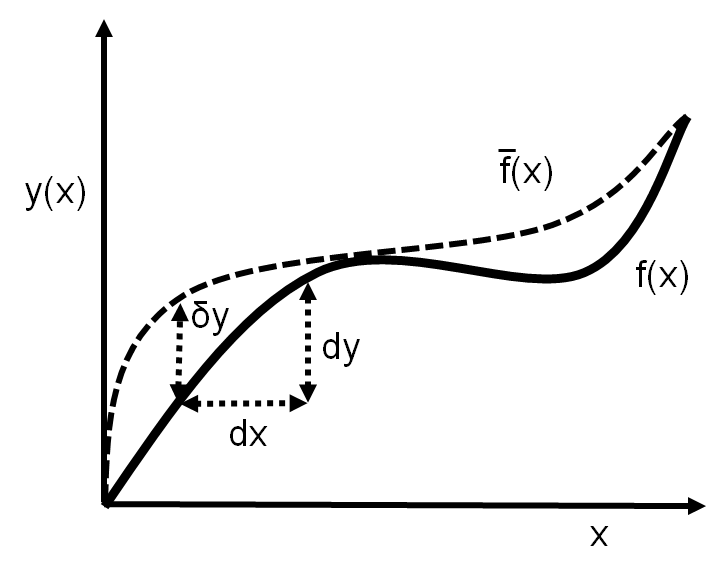
\includegraphics[width=0.5\textwidth]{figures/VirtualDisplacement.png}
\caption{\label{fig:VirtualDisplacement}A function $y=f(x)$ showing a differential change $dx$ which corresponds to a change in $x$ of $dx$. The variation of the function at a point, $\delta y$, is also shown, which is independent of a change in $x$ and leads to a different function, $\bar{f}(x)$.}
\end{figure}
For the calculus of variations, we only consider changes in the dependent variables, thus:
\begin{align}
\delta x = 0
\end{align}

\subsection{Properties of the $\delta$ operator}
\subsubsection{Commutation with differentiation}
Consider the ``derivative of the variation'':
\begin{align}
\frac{d}{dx}\delta y =\frac{d}{dx} \left[\bar{f}(x)-f(x) \right]=\frac{d}{dx} \epsilon \phi(x)=\epsilon \phi'(x)
\end{align}
where we have used an apostrophe (') to designate derivatives with respect to $x$. Now consider the ``variation of the derivative'':
\begin{align}
\delta \left(\frac{d}{dx}f(x)\right) \equiv \frac{d\bar{f}}{dx}-\frac{df}{dx} = \frac{d}{dx} (f(x)+\epsilon \phi(x)) - \frac{df}{dx} = \epsilon \phi'(x)
\end{align}
We thus find that $\delta$ is commutative with $\frac{d}{dx}$:
\begin{align}
\label{eqn:vardiffcommut}
\therefore \delta \left(\frac{dy}{dx}\right) = \frac{d}{dx}\left(\delta y\right)
\end{align}
\subsubsection{Commutation with integration}
Next, consider the variation of a definite integral:
\begin{align}
\delta \int_a^b f(x) dx &\equiv  \int_a^b \bar{f}(x) dx - \int_a^b f(x) dx = \int_a^b (\bar{f}(x)-f(x)) dx\nonumber\\
\therefore \delta \int_a^b f(x) dx &= \int_a^b \delta f(x) dx 
\end{align}
The delta operator also commutes with respect to integration.
\subsubsection{Chain Rule}
If $y$ is a function of $x$, the variation of a function, $F(y)$, is given by:
\begin{align}
\delta F(y) &= F(y+\delta y)-F(y)
\end{align}
We can expand $F(y+\delta y)$ using a Taylor series, where $\delta y$ is small:
\begin{align}
F(y+\delta y)=F(y)+\frac{dF}{dy}\delta y + \frac{1}{2!}\frac{d^2F}{dy^2}(\delta y)^2+\dots 
\end{align}
Given that $\delta y$ are small, we can ignore the terms in powers higher than 2:
\begin{align}
F(y+\delta y)&=F(y)+\frac{dF}{dy}\delta y\nonumber\\
\therefore \delta F(y)&=\frac{dF}{dy}\delta y
\label{eqn:varChainRule}
\end{align}
which is (like) the Chain Rule.
\begin{example}{0pt}{Determine $\delta(\cos{\theta})$}{}
Using the Chain Rule:
\begin{align*}
\delta(\cos{\theta})=-\sin{\theta}\delta\theta
\end{align*}
\end{example}
\noindent
If the function $F$ is a function of multiple functions, $y(x), z(x), \dots$, we proceed the same way, but using partial derivatives:
\begin{align}
\delta F(y,z,\dots) &= F(y+\delta y, z+\delta z, \dots)-F(y,z,\dots)\nonumber\\
&=\frac{\partial F}{\partial y}\delta y +\frac{\partial F}{\partial z}\delta z+\dots+ \frac{1}{2!}\left(\frac{\partial^2F}{\partial y}\delta^2y+\frac{\partial^2F}{\partial z}\delta^2z+2\frac{\partial^2 F}{\partial y\partial z}\delta y \delta z+\dots \right) +\dots
\label{eqn:varChainRuleMulti}
\end{align}
where again, we will neglect the terms in $\delta^2$ and higher.
\begin{example}{0pt}{Compare the differential displacement and virtual displacement of a position vector $\vec{r}=\vec{r}(q_1,q_2,\dots,q_n,t)$ that is a function of generalized coordinates, $q$.}{}
When considering the position of a particle as a function of the generalized coordinates:
\begin{align*}
\vec{r}=\vec{r}(q_1,q_2,\dots,q_n,t)
\end{align*}
the differential displacement (also the ``true'' displacement):
\begin{align*}
d\vec{r}=\frac{\partial\vec{r}}{\partial q_1}dq_1+\dots+\frac{\partial\vec{r}}{\partial q_n}dq_n+\frac{\partial\vec{r}}{\partial t}dt
\end{align*}
whereas the virtual displacement does not have a time differential in it:
\begin{align*}
\delta\vec{r}=\frac{\partial\vec{r}}{\partial q_1}\delta q_1+\dots+\frac{\partial\vec{r}}{\partial q_{n}}\delta q_{n}
\end{align*}
\end{example}

\section{Stationary value of a function}
In analytic mechanics, we will be interested in the stationary value of an integral. We start by considering the stationary value of a function. For example, an n-dimensional function $F(q_1, q_2, \dots, q_n)$, can be pictured as a surface in a space with n+1 dimension (for example, imagine a 2-dimensional surface in 3-dimensional space). The stationary points of the functions are locations where the surface is ``flat'', and can correspond to local ``extrema'' (minima or maxima) or ``saddle points''. We can use the formalism of variations to find the conditions for such points. 

If the point, $P$, is a stationary value of the function, $F(q_1, q_2, \dots, q_n)$, then, the variation of the function near $P$ in the direction of an arbitrary virtual displacement, $\delta\vec{q}$, is 0 (the function is flat in the infinitesimal region near the point). The variation of the function is (technically called the ``first variation'', as we drop the higher order terms in the Taylor series):
\begin{align}
\delta F&=\frac{\partial F}{\partial q_1}\delta q_1 + \frac{\partial F}{\partial q_2}\delta q_2 +\dots+\frac{\partial F}{\partial q_N}\delta q_N
\end{align}  
We can write this in terms of finite numbers if we write the virtual displacements as:
\begin{align}
\delta q_i=\epsilon \alpha_i
\end{align}
where $\vec{\alpha}$ is a vector in the direction of the virtual displacement and $\epsilon$ is a number that tends to zero. The rate of change of the function, $F$, in the direction of $\vec{\alpha}$ is:
\begin{align}
\frac{\delta F}{\epsilon}=\frac{\partial F}{\partial q_1}\alpha_1 + \frac{\partial F}{\partial q_2}\alpha_2 +\dots+\frac{\partial F}{\partial q_N}\alpha_N
\end{align} 
which must vanish for a stationary point (writing the above equation as a sum):
\begin{align}
\sum_i\frac{\partial F}{\partial q_i}\alpha_i =0
\end{align} 
In order to have a stationary point, the rate of the change of the function must vanish for any direction, $\vec{\alpha}$, so that each term must be equal to zero, independent of the $\alpha_i$:
\begin{align}
\frac{\partial F}{\partial q_i}\alpha_i &=0\nonumber\\
\therefore \frac{\partial F}{\partial q_i}&=0
\end{align}
and we recover the familiar result from calculus that the partial derivatives must vanish at $P$, for that point to be a stationary point of the function. The second order derivatives (``second variations'') are needed in order to know if this is a local minimum, maximum or saddle point. For analytic mechanics, we will generally only need to know if the point is stationary.

\section{Constraints and Lagrange multipliers}
\subsection{Single constraint}
In some cases, the problem of finding a stationary point does not generalize to any virtual displacement, as constraints between coordinates limit the choice of direction for $\vec{\alpha}$. For example, in the case finding the minimum of the potential energy of a marble in a bowl, we would have a constraint equation in the form:
\begin{align}
x^2+y^2+z^2=(R-r)^2
\end{align}
where $(x,y,z)$ are the position of the center of mass of the ball, $R$ is the radius of the bowl, and $r$ is the radius of the ball. The ball is constrained to be in the bowl, so we cannot just consider any point in space as the minimum of the potential energy.

In general then, we seek to minimize the function $F(q_1, q_2, \dots, q_n)$, subject to some constraint equation(s) between the coordinates:
\begin{align}
f(q_1, q_2, \dots, q_n)=0
\end{align}
The obvious (and valid) way to handle this is to use the constraint equation to eliminate one of the variables from $F$ and work with n-1 independent (generalized) coordinates. However, it may not be convenient to eliminate a coordinate, and there might not be an obvious choice of which coordinate should be the ``dependent'' one. Lagrange's method of multipliers allows one to preserve all the coordinates while including the constraints (or ``auxiliary conditions''). We start by finding the stationary point subject to a single auxiliary condition. We have:
\begin{align}
\delta f=\frac{\partial f}{\partial q_1}\delta q_1 + \frac{\partial f}{\partial q_2}\delta q_2 +\dots+\frac{\partial f}{\partial q_n}\delta q_n=0
\end{align}
In order to have a stationary point of $F$, we also have:
\begin{align}
\delta F=\frac{\partial F}{\partial q_1}\delta q_1 + \frac{\partial F}{\partial q_2}\delta q_2 +\dots+\frac{\partial F}{\partial q_n}\delta q_n=0
\end{align}
however, unlike in the un-constrained case, the $\delta q_i$, are not independent, thus this no longer implies that each term (and hence each partial derivative) is zero. Since the two above equations are zero, we can create a linear combination of them, which will still equal zero:
\begin{align}
&\delta F+\lambda \delta f=\frac{\partial F}{\partial q_1}\delta q_1 + \frac{\partial F}{\partial q_2}\delta q_2 +\dots+\frac{\partial F}{\partial q_n}\delta q_n + \lambda (\frac{\partial f}{\partial q_1}\delta q_1 + \frac{\partial f}{\partial q_2}\delta q_2 +\dots+\frac{\partial f}{\partial q_n}\delta q_n)=0\nonumber\\
&\sum_{i=1}^{n} \left(\frac{\partial F}{\partial q_i}+ \lambda \frac{\partial f}{\partial q_i}\right)\delta q_i=0
\end{align}
where $\lambda$ is called a ``Lagrange multiplier'', and is not known a priori. Note again that only the sum is zero, not the individual terms. We now \textbf{choose} $\lambda$ so that the n-th term is zero:
\begin{align}
\frac{\partial F}{\partial q_n}+ \lambda \frac{\partial f}{\partial q_n}=0
\end{align}
Given the chosen value of $\lambda$, the sum now contains one less term:
\begin{align}
\sum_{i=1}^{n-1} \left(\frac{\partial F}{\partial q_i}+ \lambda \frac{\partial f}{\partial q_i}\right)\delta q_i&=0
\end{align}
At this point however, we effectively imposed the constraint to eliminate $\delta q_n$; the remaining coordinates can now be varied independently (``freely''), so that the remaining terms (given $\lambda$) are individually zero:
\begin{align}
\frac{\partial F}{\partial q_i}+ \lambda \frac{\partial f}{\partial q_i}=0 \text{       (i=1, 2, \dots n-1)}
\end{align}
We thus have $n-1$ equations as above, and 1 equation to determine $\lambda$, resulting in $n$ equations to find the point where $F$ is stationary given the auxiliary condition $f=0$. By inspection, those equations are the same and the distinction between dependent and independent variables vanishes!

This method can thus be written a little bit more generally by considering all the $\delta q_i$ as independent instead of (artificially) eliminating $\delta q_n$, and considering the variation:
\begin{align}
\delta F + \lambda \delta f
\end{align}
We have:
\begin{align}
\delta (F+\lambda f) &= \delta F+ (\delta \lambda) f + \lambda (\delta f\nonumber)\\
&=\delta F + \lambda \delta f
\end{align}
since $f=0$. We can then construct a new function, $\bar{F}$:
\begin{align}
\bar{F}=F + \lambda f
\end{align}
and consider the stationary points of $\bar{F}$ without having to worry about auxiliary conditions, thus treating all variations of the coordinates as unconstrained (``free variations''). In this situation, we have n equations by setting the partial derivatives of $\bar{F}$ to zero and 1 equation from the constraint equation $f=0$. This allows us to solve for the $n$ values of $q$ at the minimum and the unknown $\lambda$.

\begin{example}{0pt}{Calculate the dimensions, $x,y,z$ of a box that maximizes the volume for a fixed surface area of 2A.}{}
We wish to maximize the volume of a box, given by:
\begin{align*}
F(x,y,z)=xyz
\end{align*}
subject to the constraint that the area is equal to 2A:
\begin{align*}
2xy+2xz+2yz=2A
\end{align*}
Therefore, the constraint can be written as:
\begin{align*}
f(x,y,z)=xy+xz+yz-A=0
\end{align*}
We thus introduce a Lagrange multiplier, $\lambda$, and minimize
\begin{align*}
\bar{F}=F+\lambda f= xyz+\lambda(xy+xz+yz-A)
\end{align*}
This gives us the 3 equations (one for each coordinate):
\begin{align*}
\frac{\partial \bar{F}}{\partial x}&=yz+\lambda(y+z)=0\\
\frac{\partial \bar{F}}{\partial y}&=xz+\lambda(x+z)=0\\
\frac{\partial \bar{F}}{\partial z}&=yx+\lambda(y+x)=0
\end{align*}
Together with the constraint equation, this gives 4 equations and 4 unknowns ($x,y,z,\lambda$). We can multiply each of the 3 equations by $x,y,z$ respectively to obtain:
\begin{align*}
xyz+x\lambda(y+z)=0\\
yxz+y\lambda(x+z)=0\\
zyx+z\lambda(y+x)=0
\end{align*}
From the first two equations:
\begin{align*}
\therefore x\lambda(y+z)=y\lambda(x+z)\\
\lambda x= \lambda y
\end{align*}
giving us the possibility that either $\lambda=0$ or $x=y$. If $\lambda=0$ anyone of the above equations imply that $xyz=0$, which corresponds to a volume of zero. In principle, our method will only give us a stationary value, and a volume of zero is indeed a minimum of the volume. However, that is not the choice of interest for us, so we choose $x=y$. Combining the other two equations gives us that $x=z$, showing us that the result is a cube. We can use the constraint equations to find the dimensions of the cube:
\begin{align*}
f(x,y,z)=xy+xz+yz-A=3x^2-A=0\nonumber\\
\therefore x=\sqrt{\frac{A}{3}}
\end{align*}
We found our solution and did not need to explicitly solve for the Lagrangian multiplier. Also note that our volume function itself has no maximum, however, the auxiliary condition results in a stationary value that is other than the minimum.
\label{ex:boxvolume}
\end{example}


\subsection{Multiple constraints}
The treatment is similar when we have multiple auxiliary conditions (say $k$ such constraints):
\begin{align}
f_1(q_1, q_2, \dots, q_n)&=0\nonumber\\
f_2(q_1, q_2, \dots, q_n)&=0\nonumber\\
\dots\nonumber\\
f_k(q_1, q_2, \dots, q_n)&=0
\end{align}
where we now have $n-k$ degrees of freedom. The variation of the auxiliary conditions are:
\begin{align}
\delta f_i=\frac{\partial f_i}{\partial q_1}\delta q_1 + \frac{\partial f_i}{\partial q_2}\delta q_2 +\dots+\frac{\partial f_i}{\partial q_n}\delta q_n=0
\end{align}
Again, we wish to find the stationary point of $F$, leading to:
\begin{align}
\delta F = \sum_{i=1}^{n}\frac{\partial F}{\partial q_i}\delta q_i=0
\end{align}
We now introduce a Lagrange multiplier $\lambda_i$ for each of the $k$ auxiliary conditions $f_i$, so that the following linear combination is still zero:
\begin{align}
\label{eqn:multilagrangemulti}
\delta F + \lambda_1 \delta f_1 +\lambda_2 \delta f_2 +\dots+\lambda_k \delta f_k&=0\nonumber\\
\sum_{i=1}^{n}\left(\frac{\partial F}{\partial q_i}+\lambda_1 \frac{\partial f_1}{\partial q_i}+\dots +\lambda_k \frac{\partial f_k}{\partial q_i}\right)\delta q_i=0
\end{align}
We now choose to solve for the $k$ Lagrange multipliers by eliminating the last $k$ terms in the sum, leading to $k$ equations for the $k$ unknown $\lambda$:
\begin{align}
\label{eqn:multilagrangemulti2}
&\frac{\partial F}{\partial q_n}+\lambda_1 \frac{\partial f_1}{\partial q_n}+\dots +\lambda_k \frac{\partial f_k}{\partial q_n}=0\nonumber\\
&\frac{\partial F}{\partial q_{n-1}}+\lambda_1 \frac{\partial f_1}{\partial q_{n-1}}+\dots +\lambda_k \frac{\partial f_k}{\partial q_{n-1}}=0\nonumber\\
&\frac{\partial F}{\partial q_{n-2}}+\lambda_1 \frac{\partial f_1}{\partial q_{n-2}}+\dots +\lambda_k \frac{\partial f_k}{\partial q_{n-2}}=0\nonumber\\
&\dots \nonumber\\
&\frac{\partial F}{\partial q_{n-k+1}}+\lambda_1 \frac{\partial f_1}{\partial q_{n-k+1}}+\dots +\lambda_k \frac{\partial f_k}{\partial q_{n-k+1}}=0
\end{align}
The rest of the $n-k$ coordinates in equation \ref{eqn:multilagrangemulti} can now be varied freely, so that each corresponding terms in the sum must vanish:
\begin{align}
\sum_{i=1}^{n-k}\left(\frac{\partial F}{\partial q_i}+\lambda_1 \frac{\partial f_1}{\partial q_i}+\dots +\lambda_k \frac{\partial f_k}{\partial q_i}\right)\delta q_i=0
\end{align}
thus giving us $n-k$ equations:
\begin{align}
&\frac{\partial F}{\partial q_1}+\lambda_1 \frac{\partial f_1}{\partial q_1}+\dots +\lambda_k \frac{\partial f_k}{\partial q_1}=0\nonumber\\
&\frac{\partial F}{\partial q_2}+\lambda_1 \frac{\partial f_1}{\partial q_2}+\dots +\lambda_k \frac{\partial f_k}{\partial q_2}=0\nonumber\\
&\dots \nonumber\\
&\frac{\partial F}{\partial q_{n-k}}+\lambda_1 \frac{\partial f_1}{\partial q_{n-k}}+\dots +\lambda_k \frac{\partial f_k}{\partial q_{n-k}}=0
\end{align}
Again, by inspection, these equations are the same as those in equation \ref{eqn:multilagrangemulti2}, removing any distinction between dependent and independent variables. We can thus construct the function $\bar{F}$:
\begin{align}
\bar{F}=F+\lambda_1 f_1+\lambda_2 f_2 +\dots +\lambda_k f_k
\end{align}
and treat all of the coordinates in the same way. That is, instead of performing the variation of $F$ subject to the auxiliary conditions, we can perform the variation on $\bar{F}$ and ``ignore'' the auxiliary conditions. This gives us the $n$ equations:
\begin{align}
\frac{\partial F}{\partial q_i}+\lambda_1 \frac{\partial f_i}{\partial q_i}+\dots +\lambda_k \frac{\partial f_k}{\partial q_i}=0 \text{        (i=0\dots n)}
\end{align}
together with the $k$ constraint equations to determine the $n$ coordinates $q_i$ and the $k$ Lagrange multipliers.
\section{Stationary value of an integral}
In analytic mechanics, we will find that we need to find the stationary value of an integral. For example, we may need to find the curve $y(x)$ that results in the definite integral of some function $L(y,y',x)$ being maximized (or stationary). We called the definite integral, $I$, a ``functional'':
\begin{align}
I = \int_a^b L(y,y',x)dx
\end{align}
One common example is the ``Brachistochrone'' problem, in which we wish to find the shape of a wire, $y(x)$, that minimizes the time for a frictionless bead to slide down under gravity from some point $a$ to another point $b$. This problem in fact led to the development of the field of variational calculus.
\begin{example}{0pt}{Derive the functional corresponding to a bead sliding under gravity down a frictionless wire given by the function $y(x)$}{\capfig{0.3\textwidth}{figures/bchrone.png}{Bead sliding under gravity on a wire from a to b.}}
The time that it takes to slide down the path is given by the integral of the time it takes to slide down an infinitesimal arc, $ds$:
\begin{align*}
T=\int_a^b \frac{ds}{v}
\end{align*}
where v is the instantaneous speed. The speed is easily found by conservation of energy. If the bead started at rest:
\begin{align*}
\frac{1}{2}mv^2=mg(y_a-y)\nonumber\\
\therefore v =\sqrt{2g(y_a-y)}
\end{align*}
The arc-length, $ds$, can be expressed in terms of $dx$ and $dy$:
\begin{align*}
ds=\sqrt{dx^2+dy^2}=\sqrt{1+y'^2}dx
\end{align*}
Finally, the time is given by:
\begin{align*}
T=\int_a^b \frac{\sqrt{1+y'^2}}{\sqrt{2g(y_a-y)}}dx
\end{align*}
And the problem is that of solving for the function $y(x)$ that minimizes the ``functional'' $T$, given by the definite integral of $L(y,y',x)$, where:
\begin{align*}
L(y,y',x)=\frac{\sqrt{1+y'^2}}{\sqrt{2g(y_a-y)}}
\end{align*}
\label{ex:brach}
\end{example}
\noindent
We thus want to find the condition on $L$ such that the functional, $I$, is stationary, given the boundary condition that the function, $y(x)$, passes through $a$ and $b$.

\noindent
In analogy with finding the stationary point of a function, we examine the rate of change of the functional as we vary $y(x)$. We start with the variation of the integrand:
\begin{align}
\delta L(y,y',x)=L(y+\delta y, y'+\delta y', x)-L(y,y',x)
\end{align}
where, as you recall, we do not consider any variations in $x$. We can use the first order terms in $\delta$ from a Taylor series to expand $L(y+\delta y, y'+\delta y', x)$:
\begin{align}
L(y+\delta y, y'+\delta y', x)=L(y,y',x)+\frac{\partial L}{\partial y}\delta y+\frac{\partial L}{\partial y'}\delta y'
\end{align}
Thus:
\begin{align}
\delta I &= \delta \int_a^b L(y,y',x)dx\nonumber\\
&= \int_a^b \delta L(y,y',x)dx\nonumber\\
&= \int_a^b  \left( \frac{\partial L}{\partial y}\delta y+\frac{\partial L}{\partial y'}\delta y'\right)dx
\end{align}
Recalling from equations \ref{eqn:vardef} and \ref{eqn:vardiffcommut}  that we can write:
\begin{align}
\delta y = \epsilon \phi(x)\nonumber\\
\delta y' = \epsilon \phi'(x)
\end{align}
where $\phi(x)$ is a small variation of the function $y(x)$. The functional becomes:
\begin{align}
\delta I &=\epsilon \int_a^b  \left( \frac{\partial L}{\partial y}\phi(x)+\frac{\partial L}{\partial y'}\phi'(x)\right)dx
\end{align}
Now, since we want to find a stationary value of $I$, we require the rate of change of $\delta I$ with respect to $\epsilon$ to be zero:
\begin{align}
\frac{d\delta I}{d\epsilon}=\frac{\delta I}{\epsilon} &=\int_a^b  \left( \frac{\partial L}{\partial y}\phi(x)+\frac{\partial L}{\partial y'}\phi'(x)\right)dx=0
\end{align}
The second part can be integrated by parts:
\begin{align}
\int_a^b \frac{\partial L}{\partial y'}\phi'(x)dx=\phi(x)\frac{\partial L}{\partial y'}\Big |_a^b-\int_a^b \frac{d}{dx}\left(\frac{\partial L}{\partial y'}\right)\phi(x)dx
\end{align}
The first term of integration by parts is zero, because the function $y(x)$ is fixed at the end points of the integration range, so $\phi(x=a)=\phi(x=b)=0$. We thus have:
\begin{align}
\frac{\delta I}{\epsilon} &=\int_a^b  \left( \frac{\partial L}{\partial y}\phi(x)-\frac{d}{dx}\left(\frac{\partial L}{\partial y'}\right)\phi(x)\right)dx\nonumber\\
&=\int_a^b  \phi(x)\left( \frac{\partial L}{\partial y}-\frac{d}{dx}\left(\frac{\partial L}{\partial y'}\right)\right)dx=0
\label{eqn:ELderiv}
\end{align}
The only way for this integral to vanish, regardless of the choice of $\phi(x)$ is for the remaining part of the integrand to always be zero. This leads to the ``Euler-Lagrange'' equation, which is the condition for the functional $\int L(y,y',x)dx$ to be stationary:
\begin{align}
\frac{d}{dx}\left(\frac{\partial L}{\partial y'}\right)-\frac{\partial L}{\partial y}=0
\end{align}
Noting that $\phi(x)=\delta y$, we could also have written equation \ref{eqn:ELderiv} as:
\begin{align}
\frac{\delta I}{\epsilon} &=\int_a^b  \delta y\left( \frac{\partial L}{\partial y}-\frac{d}{dx}\left(\frac{\partial L}{\partial y'}\right)\right)dx=0
\end{align}
a notation which we will find convenient in the next section. 


\noindent
In analytic mechanics, we will generally have a function, $L$, that depends on multiple coordinates, $q_i$, their generalized velocities, $\dot{q}$, and time will play the role of the independent variable:
\begin{align}
L=L(q_1,q_2,\dots,\dot{q_1}, \dot{q_2},\dots,t)
\end{align}
We will want to find the values of $q_i(t)$ that lead to a stationary value of:
\begin{align}
S=\int_a^b L(q_1,q_2,\dots,\dot{q_1}, \dot{q_2},\dots,t)dt
\end{align}
Following the same procedure as above, and collecting the terms for each coordinate, we can show that we get an Euler-Lagrange equation for each coordinate:
\begin{align}
\frac{d}{dt}\left(\frac{\partial L}{\partial \dot{q}_i}\right)-\frac{\partial L}{\partial q_i}=0 \text{              (i=1\dots n)}
\end{align}


\section{Stationary value of an integral that does not explicitly depend on x}
We consider the special case when the function $L$ does not depend explicitly on $x$ (that is, it still depends explicitly on the functions $y(x)$ and $y'(x)$):
\begin{align}
L&=L(y,y')\nonumber\\
\frac{\partial L}{\partial x}&=0
\end{align}
Consider the following identity:
\begin{align}
\frac{d}{dx}\left(y'\frac{\partial L}{\partial y'} -L \right)&=y''\frac{\partial L}{\partial y'}+y' \frac{d}{dx}\left(\frac{\partial L}{\partial y'}\right)- \frac{dL}{dx}\nonumber\\
&=y''\frac{\partial L}{\partial y'}+y' \frac{d}{dx}\left(\frac{\partial L}{\partial y'}\right)-\left(\frac{\partial L}{\partial y}\frac{dy}{dx}+\frac{\partial L}{\partial y'}\frac{dy'}{dx} +\frac{\partial L}{\partial x} \right)\nonumber\\
&=y''\frac{\partial L}{\partial y'}+y' \frac{d}{dx}\left(\frac{\partial L}{\partial y'}\right)-\left(\frac{\partial L}{\partial y}y'+\frac{\partial L}{\partial y'}y''  \right)\nonumber\\
&=y'\left[ \frac{d}{dx}\left(\frac{\partial L}{\partial y'}\right)-\frac{\partial L}{\partial y}\right]
\end{align}
where we have used the fact that:
\begin{align}
dL=\frac{\partial L}{\partial y}dy+\frac{\partial L}{\partial y'}dy' +\frac{\partial L}{\partial x}dx 
\end{align}
where the last term is zero.

If the function $L$ satisfies the Euler-Lagrange equations, this implies that:
\begin{align}
\frac{d}{dx}\left(y'\frac{\partial L}{\partial y'} -L \right)&=0\nonumber\\
\therefore y'\frac{\partial L}{\partial y'} -L =k
\label{eqn:varnox}
\end{align}
where $k$ is a constant. This is equivalent to the Euler-Lagrange equations for the case where $L$ does not explicitly depend on $x$. It is an easier equation to solve for $y(x)$, since it only contains first order derivatives. 

\subsection{The case when there are multiple functions}
Suppose that the function $L$ depends on multiple functions $y_1(x),\dots, y_n(x)$ and their derivatives, $y'_1(x),\dots, y'_n(x)$, $L=L(y_1(x),\dots, y_n(x),y'_1(x),\dots, y'_n(x))$. If $L$ does not explicitly depend on $x$, we have:
\begin{align}
\frac{dL}{dx}&=\frac{\partial L}{\partial y_1}y'_1+\dots +\frac{\partial L}{\partial y_n}y'_n+
\frac{\partial L}{\partial y'_1}y''_1+\dots +\frac{\partial L}{\partial y'_n}y''_n\nonumber\\
&=\sum_{i=1}^n\left(\frac{\partial L}{\partial y_i}y'_i+\frac{\partial L}{\partial y'_i}y''_i \right)
\end{align}
We thus consider the identity:
\begin{align}
\frac{d}{dx}\left(\sum_{i=1}^n\left( y_i'\frac{\partial L}{\partial y_i'}\right) -L \right)&=\sum_{i=1}^n\left( y_i''\frac{\partial L}{\partial y_i'}+y_i'\frac{d}{dx}\frac{\partial L}{\partial y_i'}\right)-\frac{dL}{dx}\nonumber\\
&=\sum_{i=1}^n\left( y_i''\frac{\partial L}{\partial y_i'}+y_i'\frac{d}{dx}\frac{\partial L}{\partial y_i'}\right)-\sum_{i=1}^n\left(\frac{\partial L}{\partial y_i}y'_i+\frac{\partial L}{\partial y'_n}y''_n \right)\nonumber\\
&=\sum_{i=1}^n\left(y'_i\left[\frac{d}{dx}\frac{\partial L}{\partial y_i'}- \frac{\partial L}{\partial y_i} \right]  \right)
\end{align}
Again, the term on the right is zero since the Euler-Lagrange equations are satisfied by each $y_i(x)$. We thus obtain the equivalent result as we did with a single function (noting that we have a sum on the left):
\begin{align}
\frac{\partial L}{\partial x}=0\nonumber\\
\therefore \sum_{i=1}^n\left( y_i'\frac{\partial L}{\partial y_i'}\right) -L=k
\label{eqn:varnoxm}
\end{align}
where $k$ is a constant.


\section{Stationary value of an integral with auxiliary conditions}
We conclude this chapter by consider the stationary value of a functional with integrand, $L(q_1,q_2,\dots,\dot{q_1}, \dot{q_2},\dots,t)$, subject to $k$ constraints on the, $q_i(t)$, functions. Here, in analogy with mechanics, we chose $q(t)$ and $\dot q(t)$ as functions that depend on the independent variable, $t$ (instead of $y(x)$ as we had in the previous section).
\begin{align}
f_1(q_1, q_2, \dots, q_n, t)&=0\nonumber\\
f_2(q_1, q_2, \dots, q_n, t)&=0\nonumber\\
\dots\nonumber\\
f_k(q_1, q_2, \dots, q_n, t)&=0
\end{align}
where the constraints depend on time. As before, it would be possible to eliminate $k$ of the $q_i(t)$ functions, but this may not be the most mathematically convenient and may arbitrarily make some functions ``dependent'' and others ``independent''. Instead, we can use the method of the Lagrangian multipliers. The variation of the constraints are zero for all times:
\begin{align}
\delta f_1&=\frac{\partial f_1}{\partial q_1}\delta q_1 + \frac{\partial f_1}{\partial q_2}\delta q_2 +\dots+\frac{\partial f_1}{\partial q_n}\delta q_n=0\nonumber\\
\delta f_2&=\frac{\partial f_2}{\partial q_1}\delta q_1 + \frac{\partial f_2}{\partial q_2}\delta q_2 +\dots+\frac{\partial f_2}{\partial q_n}\delta q_n=0\nonumber\\
\dots\nonumber\\
\delta f_k&=\frac{\partial f_k}{\partial q_1}\delta q_1 + \frac{\partial f_k}{\partial q_2}\delta q_2 +\dots+\frac{\partial f_k}{\partial q_n}\delta q_n=0
\label{eqn:varconstraints}
\end{align}
We can then construct a new functional of which we want to find a stationary value:
\begin{align}
\delta I = \int_{t_a}^{t_b}  \delta L(q_1,q_2,\dots,\dot{q_1}, \dot{q_2},\dots,t)dt+\int_a^b (\lambda_1 \delta f_1+\lambda_2 \delta f_2 +\dots +\lambda_k \delta f_k)dt=0
\end{align}
where we have effectively added zero to our original functional. Note that the $\lambda_i$ are in principle functions of $t$, since the $f_i$ are functions of t. The first term of the variation, after integration by parts will have a term containing $\delta q_i$ of the form:
\begin{align}
\int_{t_a}^{t_b}  \left(\frac{d}{dt}\left(\frac{\partial L}{\partial \dot{q}_i}\right)-\frac{\partial L}{\partial q_i}\right) \delta q_i dt
\end{align}
and there will be a matching term in the part with the Lagrange multipliers:
\begin{align}
\int_{t_a}^{t_b}  \left(\lambda_1 \frac{\partial f_1}{\partial q_i}+\lambda_2\frac{\partial f_2}{\partial q_i} +\dots +\lambda_k \frac{\partial f_k}{\partial q_i} \right) \delta q_i dt
\end{align}
This results in the functional being
\begin{align}
\delta I=\sum_{i=1}^n \int_a^b\left[ \left(\frac{d}{dt}\left(\frac{\partial L}{\partial \dot{q}_i}\right)-\frac{\partial L}{\partial q_i}\right) +\left(\lambda_1 \frac{\partial f_1}{\partial q_i}+\lambda_2\frac{\partial f_2}{\partial q_i} +\dots +\lambda_k \frac{\partial f_k}{\partial q_i} \right)\right] \delta q_i dt
\end{align}
In principle, the term in square brackets is \textbf{not} zero, because the $\delta q_i$ cannot all be varied independently because of the constraint equations \ref{eqn:varconstraints}. We can however \textbf{choose} the $\lambda_i$ such that the last $k$ terms are zero:
\begin{align}
\left[ \left(\frac{d}{dt}\left(\frac{\partial L}{\partial \dot{q}_i}\right)-\frac{\partial L}{\partial q_i}\right) +\left(\lambda_1 \frac{\partial f_1}{\partial q_i}+\lambda_2\frac{\partial f_2}{\partial q_i} +\dots +\lambda_k \frac{\partial f_k}{\partial q_i} \right)\right]=0 \text{  			(i=n-k+1\dots n)}
\label{eqn:ELLambda}
\end{align}
Now, this leaves us with the remaining $n-k$ terms for which the $\delta q_i$, can be varied independently. Of course, the whole point of the Lagrange multiplier method is that this gives equations that are identical for all $q_i$, removing the distinction between dependent and independent variables. The above equation is thus true for all values of $i=1\dots n$!

We can thus re-express the problem of varying the integrand $L$ subject to auxiliary conditions as the equivalent problem of varying a modified integrand, $L'$, without worrying about auxiliary conditions:
\begin{align}
L'=L-(\lambda_1f_1+\lambda_2f_2+\dots +\lambda_kf_k)
\end{align}
where the auxiliary conditions can be used in addition to the Euler-Lagrange equations to determine all of the $q_i(t)$ and the $\lambda_i(t)$. This leads to the Euler-Lagrange equations which we can re-write as:
\begin{align}
\left(\frac{d}{dt}\left(\frac{\partial L}{\partial \dot{q}_i}\right)-\frac{\partial L}{\partial q_i}\right) &=-\lambda_1 \frac{\partial f_1}{\partial q_i}-\lambda_2\frac{\partial f_2}{\partial q_i} -\dots -\lambda_k \frac{\partial f_k}{\partial q_i}\nonumber\\
\left(\frac{d}{dt}\left(\frac{\partial L}{\partial \dot{q}_i}\right)-\frac{\partial L}{\partial q_i}\right) &=-\sum_{j=1}^k\lambda_j \frac{\partial f_j}{\partial q_i}\nonumber\\
\left(\frac{d}{dt}\left(\frac{\partial L}{\partial \dot{q}_i}\right)-\frac{\partial L}{\partial q_i}\right) &=Q_i
\label{eqn:ELLambdaQ}
\end{align}
where we have introduced:
\begin{align}
Q_i\equiv -\sum_{j=1}^k\lambda_j \frac{\partial f_j}{\partial q_i}
\end{align}
and the overall negative sign is not important, since the Lagrange multipliers can be chosen.


\begin{example}{0pt}{Show that the Euler-Lagrange equation for $L'=L-\lambda_1f_1-\lambda_2f_2-\dots -\lambda_kf_k$ is equivalent to equation \ref{eqn:ELLambda}. That is, show that the sign in front of the Lagrange multipliers is arbitrary.}{}
\begin{align*}
&\frac{d}{dt}\left(\frac{\partial L'}{\partial \dot{q}_i}\right)-\frac{\partial L'}{\partial q_i}\nonumber\\
&=\frac{d}{dt}\left(\frac{\partial}{\partial \dot{q}_i}(L-\lambda_1f_1-\dots -\lambda_kf_k)\right)-\frac{\partial}{\partial q_i}(L-\lambda_1f_1-\dots -\lambda_kf_k)\nonumber\\
\end{align*}
The $\lambda_if_i$ terms do not explicitly depend on $\dot{q}_i$, and the $\lambda_i$ do not depend on the $q_i$:
\begin{align*}
&=\frac{d}{dt}\left(\frac{\partial L}{\partial \dot{q}_i}\right)-\frac{\partial}{\partial q_i}(L-\lambda_1f_1-\dots -\lambda_kf_k)\nonumber\\
&=\frac{d}{dt}\left(\frac{\partial L}{\partial \dot{q}_i}\right)-\frac{\partial L}{\partial q_i}+\lambda_1\frac{\partial f_1}{\partial q_i}+\dots +\lambda_k\frac{\partial f_k}{\partial q_i}
\end{align*}
where we have a minus sign on all the Lagrange multipliers compared to equation \ref{eqn:ELLambda}, which is ok, since we are free to choose them.
\end{example}

\subsection{Case when auxiliary condition is in the form of an integral}
In certain cases, the auxiliary condition may be in the form of an integral:
\begin{align}
\int_{t_a}^{t_b} f(q_1,q_2,\dots,t)dt=C
\end{align}
where $C$ is a constant, and there may be any number of such constraint equations. Again, we can take the variation of this integral:
\begin{align}
\delta\int_{t_a}^{t_b} f(q_1,q_2,\dots,t)dt&=\int_{t_a}^{t_b} \sum \die{f}{q_i}\delta q_i dt=0
\end{align}
which must be zero. We can thus use a Lagrange multiplier and add the variation of the constraint to our original integral:
\begin{align}
&\delta\int_{t_a}^{t_b}  L(q_1,q_2,\dots,\dot{q_1}, \dot{q_2},\dots,t)dt+\lambda\delta\int_{t_a}^{t_b} f(q_1,q_2,\dots,t)dt\nonumber\\&=\delta \int_{t_a}^{t_b}\left[L(q_1,q_2,\dots,\dot{q_1}, \dot{q_2},\dots,t)+\lambda f(q_1,q_2,\dots,t)\right] dt
\end{align}
We can solve this problem by considering the stationary value of a new function, $\bar L$:
\begin{align}
\bar L(q_1,q_2,\dots,\dot{q_1}, \dot{q_2},\dots,t)\equiv L(q_1,q_2,\dots,\dot{q_1}, \dot{q_2},\dots,t)+\lambda f(q_1,q_2,\dots,t)
\end{align}
and apply the Euler-Lagrange equation to $\bar L$.



\section{Problems}
\begin{problem}{Highest point on a surface} Find the coordinates of the highest point on the surface given by $z(x,y)=x^2y+xy$ that when projected onto the xy-plane lies on a circle of radius $r=5$ centered at $x=2$ and $y=3$. Use a computer to illustrate the result. You will also likely need to solve the equations numerically.
\label{prob_CalcVar_1}
\end{problem}
\begin{problem}{Box with no lid} Find the dimensions that maximize the volume of a box with no lid, if the total surface area of the box is 1\,m$^2$.
\label{prob_CalcVar_2}
\end{problem}
%\begin{problem}{Hanging Beads} The figure shows 3 beads of equal mass $m$, connected by mass-less inextensible strings of length $l$ over a precipice of length $L$.
%\capfig{0.4\textwidth}{figures/HangingBeads.png}{3 beads of equal mass $m$, connected by mass-less inextensible strings of length $l$ over a precipice of length $L$} 
%
%\textbf{a)} Minimize the potential energy of the system to find the positions ($x_i$, $y_i$) of the 3 beads.
%
%\textbf{b)} Generalize the result from part a) if there are N beads
%
%\textbf{c)} If the beads and strings are replaced by a heavy rope with a mass per unit length of $\mu$, find the differential equation for the curve that describes the shape of the rope and use a computer to plot it.
%\end{problem}

\begin{problem}{Euler-Lagrange equations for integrand that depends on more than one function}\label{prob_CalcVar_3} Show that the stationary value of the functional $S=\int_a^b L(q_1(t),q_2(t),\dots,\dot{q_1}, \dot{q_2},\dots,t)dt$ gives an Euler-Lagrange equation for each $q_i(t)$:
\begin{align*}
\frac{d}{dt}\left(\frac{\partial L}{\partial \dot{q_i}}\right)-\frac{\partial L}{\partial q_i}=0
\end{align*}
\end{problem}

\begin{problem}{Euler-Lagrange equation when there is a second order derivative}\label{prob_CalcVar_4} Show that the equivalent of the Euler-Lagrange equation when the function in the integrand depends on the second derivative of $y$:
\begin{align*}
I=\int_a^b L(y,y',y'',x)dx
\end{align*}
is given by:
\begin{align*}
\frac{d^2}{dx^2}\die{L}{y''}-\frac{d}{dx}\die{L}{y'}+\die{L}{y}=0
\end{align*}
Note that you will have to integrate by parts twice and that the variation of $y'(x)$ is zero at the end points of the integral.
\end{problem}

\begin{problem}{Brachistrochrone}\label{prob_CalcVar_5}Refer to the problem of example \ref{ex:brach}.\\
\textbf{a)} Find the differential equation for the function $y(x)$ that solves the brachistrochrone problem, by minimizing $T$:
\begin{align*}
\sqrt{2g}T=\int_0^{x_b} \frac{\sqrt{1+y'^2}}{\sqrt{y}}dx
\end{align*}
Note that we have set the problem up such that one end of the wire is at the origin, gravity is in the positive $y$ direction, and the constant $2g$ will not change the shape of the wire. Note that a closed form solution in the form $y=f(x)$ is not possible, and only parametric solutions can be obtained (so called ``cycloids'').

\textbf{b)} Repeat part a), with the wire being constrained to have a length of $L$.
\end{problem}

\begin{problem}{Geodesic}\label{prob_CalcVar_6} Determine the functional for the shortest distance between two points on a sphere of radius $a$, and write the differential equation that gives the function $\phi(\theta)$, where $\phi$ and $\theta$ are the azimuthal and polar angles in spherical coordinates, respectively.
\end{problem}

\begin{problem}{Straight line}\label{prob_CalcVar_7} Show that the shortest distance between two points in a plane is a straight line.
\end{problem}

\begin{problem}{Catenary}\label{prob_CalcVar_8} A rope of uniform linear mass density, $\mu$, and total length, $L$, is hung across a precipice of length, $H$ (both sides of the precipice are at the same height). Minimize the potential energy of the rope:
\begin{align*}
V=\int_0^H \mu g y ds
\end{align*} 
to obtain the differential equation for the shape of the rope. Use a computer to solve and plot the resulting curve (choose reasonable values).
\end{problem}

\begin{problem}{Surface and volume of revolution}\label{prob_CalcVar_9}
\textbf{a)} Find the shape of the curve, $y(x)$, passing through two points, $a$ and $b$, that gives the minimal surface of revolution when rotated about the x-axis (see figure). Note that this would be the shape of a soap film formed between two hoops.\\
\textbf{b)} Find the shape of the curve, $y(x)$, passing through two points, $a$ and $b$, that creates a solid of revolution with the minimal moment of inertia about the x-axis (see figure). Assume that the volume is made of a material with uniform density. It will not be possible to get a closed form, write the solution as a differential equation for $y(x)$ or give $x$ in terms of an integral over $y$.
\capfig{0.2\textwidth}{figures/SurfaceOfRevolution.png}{Minimal surface of revolution between two points, problem \ref{prob_CalcVar_9}}\\
\end{problem}

\section{Solutions}

\paragraph{Problem \ref{prob_CalcVar_1}:}
\begin{solution}
\textbf{a)}
 \begin{align*}
2+2=4
\end{align*}
\end{solution}


%Copyright 2016 R.D. Martin
%This book is free software: you can redistribute it and/or modify it under the terms of the GNU General Public License as published by the Free Software Foundation, either version 3 of the License, or (at your option) any later version.
%
%This book is distributed in the hope that it will be useful, but WITHOUT ANY WARRANTY; without even the implied warranty of MERCHANTABILITY or FITNESS FOR A PARTICULAR PURPOSE.  See the GNU General Public License for more details, http://www.gnu.org/licenses/.
\chapter{Virtual work and D'Alembert's principle}
One of the advantages of analytic mechanics is that it removes the need to deal with ``internal forces''. Consider the problem of two masses attached by a rigid mass-less rod; in vector mechanics, one needs to know the tension in the rod to be able to write the forces on each mass and obtain the equation of motion. In principle, the rod itself is made of an almost infinite number of particles each exerting forces on each other, and a complete vectorial approach is not tractable. In analytic mechanics, we can distinguish ``internal forces'' and usually ignore them. Typically, these internal forces can be handled easily by using a constraint (e.g. the rod is a rigid object).

\section{Virtual work}
Virtual work, $\delta W_i$ is the work done by a force, $\vec{F}_i$ given a ``reversible virtual displacement'' that is in harmony with the given constraints, $\delta\vec{r}_i$:
\begin{align}
\delta W_i = \vec{F}_i\cdot\delta\vec{r}_i
\end{align}
A reversible displacement is one where $\delta\vec{r}_i$ can be replaced with $-\delta\vec{r}_i$ without violating any of the constraints $\delta\vec{r}_i$ is the variation of the position vector where the force is applied.  By definition, a virtual displacement that is parallel to a normal force is not reversible.

\subsection{Principal of virtual work and static equilibrium}
The principle of virtual work states that for a static equilibrium, the sum of virtual work done by all forces is equal to zero.
\begin{align}
\sum_{i=1}^N\delta W_i &= 0 \nonumber\\
\sum_{i=1}^N\vec{F}_i\cdot\delta\vec{r}_i &= 0
\end{align}
We can divide this up into ``external forces'' (such as gravity, electric fields), $\vec{F}^E_i$, and ``internal forces'' (such as tension in a rod, normal reaction forces), $\vec{F}^I_j$.
\begin{align}
\sum_{i=1}^N\delta W_i=\sum_{i=1}^N \vec{F}^E_i\cdot\delta\vec{r}_i + \sum_{i=1}^N\vec{F}^I_j\cdot\delta\vec{r}_j
\end{align}

Typically, the internal forces are related to constraints. ``Workless constraints'' are those that lead to forces that do no virtual work.
\begin{example}{0pt}{The tension force in a rigid rod that holds two masses together is workless}{\capfig{0.2\textwidth}{figures/2MassesAndRod.png}{\label{fig:2MassesAndRod}Two masses constrained by a mass-less rigid rod.}}
The tension forces on each mass are equal and opposite (Newton's third law):
\begin{align*}
\vec{F}_1=-\vec{F}_2
\end{align*}
Furthermore, the constraint that the rods be fixed relative to each other requires that their virtual displacement be the same:
\begin{align*}
\left|\vec{r}_2-\vec{r}_1\right|=l\nonumber\\
\delta \left|\vec{r}_2-\vec{r}_1\right|=\delta l=0\nonumber\\
\therefore \delta\vec{r}_1=\delta \vec{r}_2
\end{align*}
Thus, the virtual work done by the internal forces in this case is zero:
\begin{align*}
\sum\vec{F}^I_j\cdot\delta\vec{r}_j&=\vec{F}_1\cdot\delta\vec{r}_1+\vec{F}_2\cdot\delta\vec{r}_2\nonumber\\
&=\vec{F}_1\cdot\delta\vec{r}_1-\vec{F}_1\cdot\delta\vec{r}_1=0
\end{align*}
\end{example}
\begin{example}{0pt}{The normal force on a frictionless surface is workless}{\capfig{0.2\textwidth}{figures/BlockOnSurface.png}{Block on a surface}}
If the block is constrained to slide on the surface, the normal force is perpendicular to $\delta \vec{r}$ and thus does no virtual work. $\delta \vec{r}$ must be parallel to the contact surface, since it would not be reversible otherwise.
\end{example}

In the case of workless constraints, the total virtual work is given by the work of the external forces. It is generally true (although difficult to prove) that most constraint forces are workless and can be ignored.

For static equilibrium, the ``Principal of Virtual Work'' states that the total virtual work (which is done by external forces) must be zero:
\begin{align}
\therefore \sum_{i=1}^N\delta W_i=\sum_{i=1}^N \vec{F}^E_i\cdot\delta\vec{r}_i = 0 \text{   (workless constraints)}
\end{align}
This is in contrast to the vectorial approach with requires the sum of all forces (external and internal) to be zero.

\subsection{Generalized forces}
We continue by ignoring the internal forces and consider the virtual work done by N external forces:
\begin{align}
\sum_{i=1}^N\delta W_i=\sum_{i=1}^N \vec{F}^E_i\cdot\delta\vec{r}_i = 0 
\end{align}
If we have $n$ degrees of freedom, we can re-write this in terms of the generalized coordinates (where holonomic constraints are used to reduce the number of coordinates, and the coordinates are thus all independent):
\begin{align}
\vec{r}_i&=\vec{r}_i(q_1,\dots , q_n)\nonumber\\
\delta \vec{r}_i&= \sum_{j=1}^n\frac{\partial\vec{r}_i}{\partial q_j}\delta q_j\nonumber\\
\therefore \sum_{i=1}^N\delta W_i&=\sum_{i=1}^N\vec{F}^E_i\cdot\left(\sum_{j=1}^n\frac{\partial\vec{r}_i}{\partial q_j}\delta q_j\right)\nonumber\\
\sum_{i=1}^N\delta W_i&=\sum_{j=1}^n\left(\sum_{i=1}^N\vec{F}^E_i\cdot\frac{\partial\vec{r}_i}{\partial q_j}\right)\delta q_j\nonumber\\
\sum_{i=1}^N\delta W_i&=\sum_{j=1}^nQ_j\delta q_j\nonumber\\
\end{align}
where we have introduced the components, $Q_j$, of the ``generalized force'' which do not necessarily have the dimensions of force:
\begin{align}
Q_j\equiv \sum_{i=1}^N\vec{F}^E_i\cdot\frac{\partial\vec{r}_i}{\partial q_j}
\label{eqn:genforce}
\end{align}
The total work is thus the scalar product of the generalized force, $\vec Q$, and a virtual displacement vector, $\delta \vec q$, in configuration space:
\begin{align}
\sum_{i=1}^N\delta W_i=\vec{Q}\cdot\delta\vec{q}
\end{align}
If any displacement is allowed in configuration space, $\delta \vec{q}$, then all components of the generalized force must be zero for static equilibrium. In a holonomic system, where all coordinates are independent of each other, $\delta {q}_i$ all correspond to allowed displacements and the generalized force components are therefore zero. Another way to picture this is that, given generalized coordinates $q_j$, the generalized force $Q_j$ is the force that does work $Q_j \delta q_j$ when the system is displaced in the direction $\delta q_j$. Since $q_j$ is not necessarily a cartesian coordinate (it could be an angle),  $Q_j$ does not necessarily have the units of force.

\subsection{Using the Principal of Virtual Work to solve statics problems}
We proceed with a few examples for solving statics problems using the principal of virtual work. The general procedure will be as follows:
\begin{enumerate}
\item Identify the number of degrees of freedom and choose generalized coordinates 
\item Identify the forces that can perform virtual work (forces acting at points where a virtual displacement is possible given the constraints, and forces that are not perpendicular to the allowable virtual displacements)
\item Write the position vectors of the points where the forces are applied in terms of the generalized coordinates. Then, take the variations in those vectors to obtain the $\delta \vec r_i$
\item Write out the virtual work and set it to zero
\item (Alternatively) Evaluate the components of the generalized force and set them equal to zero
\end{enumerate}


\begin{example}{0pt}{What is the magnitude, $F$, of the horizontal force required to maintain a pivoting bar (restricted to pivot in a plane) of mass $m$, length $2L$, and negligible diameter (see Figure \ref{fig:PivotingBar}) at an angle $\theta$?}{\capfig{0.3\textwidth}{figures/PivotingBar.png}{\label{fig:PivotingBar}A pivoting bar, held in static equilibrium by a force, $F$.}}
This is a rigid body, so in principle there are 6 degrees of freedom. If we choose a coordinate system at the pivot point, we can describe the position of the bar by the cartesian coordinates of the pivoting end of the bar, and 3 angles to describe the rotation of the bar about the 3 axes. However, we have the following constraints:
\begin{align*}
x&=0\nonumber\\
y&=0\nonumber\\
z&=0\nonumber\\
\theta_x &=0\nonumber\\
\theta_y &=0\nonumber\\
\end{align*}
we are thus left with 1 degree of freedom. We choose $\theta=\theta_z$ as the one generalized coordinate. Next we consider the virtual work of the forces that can perform non-zero virtual work (the forces at the pivot point cannot perform any virtual work, as the pivot point cannot be moved; its virtual displacement would not be in harmony with the constraints). We have gravity and $F$ that do virtual work:
\begin{align*}
\delta W = mg\hat y\cdot\delta\vec{r}_1-F\hat x\cdot\delta\vec{r}_2
\end{align*}
The virtual displacement vectors must be consistent with the kinematic constraints, that is, they are perpendicular to the rod (and the constraints require that $\delta\vec{r}_1$ and $\delta\vec{r}_2$ point in the same direction). We can write the position vectors for the points where the forces are applied and take their variation with respect to $\theta$:
\begin{align*}
\vec{r}_1=L(-\sin{\theta}\hat{x}+\cos{\theta}\hat{y})\\
\vec{r}_2=2L(-\sin{\theta}\hat{x}+\cos{\theta}\hat{y})\\
\therefore \delta\vec{r}_1=L(-\cos{\theta}\hat{x}-\sin{\theta}\hat{y})\delta\theta\\
\therefore \delta\vec{r}_2=2L(-\cos{\theta}\hat{x}-\sin{\theta}\hat{y})\delta\theta\\
\end{align*}
Thus:
\begin{align*}
\sum_{i=1}^N\delta W_i = -mgL\sin{\theta}\delta\theta+ 2LF\cos{\theta}\delta\theta
\end{align*}
Setting the virtual work to zero, we get the same answer as you would using introductory mechanics techniques (e.g. torques):
\begin{align*}
F=\frac{1}{2}mg\tan{\theta}
\end{align*}
Let's calculate the generalized force:
\begin{align*}
Q_j&\equiv \sum_{i=1}^N\vec{F}_i\cdot\frac{\partial\vec{r}_i}{\partial q_j}\nonumber\\
\end{align*}
Note that $N=2$ and there is only 1 $q_j$, namely $\theta$. If we write the vectors in the xy coordinates, we can evaluate the partial derivatives:
\begin{align*}
\frac{\partial\vec{r}_i}{\partial \theta}&=L(-\cos{\theta}\hat{x}-\sin{\theta}\hat{y}) \\
\frac{\partial\vec{r}_2}{\partial \theta}&=2L(-\cos{\theta}\hat{x}-\sin{\theta}\hat{y})\\
\end{align*}
The generalized force is then given by:
\begin{align*}
Q_\theta&=m\vec{g}\cdot\left(L(-\cos{\theta}\hat{x}-\sin{\theta}\hat{y})\right)+\vec{F}\cdot\left(2L(-\cos{\theta}\hat{x}-\sin{\theta}\hat{y})\right)\\
&=-Lmg\sin{\theta}+2LF\cos{\theta}
\end{align*}
And you may recognize that the generalized force in the $\theta$ direction is the total torque! The requirement that the generalized force be zero is the same as requiring that the sum of the torques are zero.
\end{example}

\begin{example}{0pt}{Find the magnitude of the force, $F$, required to keep the system in equilibrium from Figure \ref{fig:BlocksOnCorner} at an angle $\theta$. The blocks of mass $m$ slide with no friction and are held by a mass-less rigid rod of length, $L$. Their dimensions are negligible.}{\capfig{0.3\textwidth}{figures/BlocksOnCorner.png}{\label{fig:BlocksOnCorner}Two blocks constrained by a massless rigid rod, held in equilibrium by a force $F$.}}
Since we have 2 particles, we have 6 possible degrees of freedom. However, each particle is constrained to move along only 1 axis, thus reducing the number of degrees of freedom by 4. Furthermore, the particles are connected by a rigid rod, which further reduces the number of degrees or freedom by 1. There is only 1 degree of freedom, and we choose $\theta$ as our generalized coordinates. The constraint equations are:
\begin{align*}
x_1&=0\nonumber\\
z_1&=0\nonumber\\
y_2&=0\nonumber\\
z_2&=0\nonumber\\
y_1^2+x_2^2&=L^2\\
\end{align*}
We have 2 forces that can perform virtual work: gravity on particle 1 and $F$ on particle 2. Gravity on particle 2 cannot perform virtual work as it is perpendicular to the allowable virtual displacements of particle 2.
\begin{align*}
\sum_{i=1}^N\delta W_i &= m\vec{g}\cdot\delta\vec{r}_1+\vec{F}\cdot\delta\vec{r}_2\\
\end{align*}
Writing the position vectors for the points where the forces are applied and calculating their variation with respect to $\theta$:
\begin{align*}
\vec{r}_1&=0\hat{x}+L\sin{\theta}\hat{y}\\
\vec{r}_2&=L\cos{\theta}\hat{x}+0\hat{y}\\
\delta\vec{r}_1&=L\cos{\theta}\delta\theta\hat{y}\\
\delta\vec{r}_2&=-L\sin{\theta}\delta\theta\hat{x} \\
\end{align*}
The virtual work is then:
\begin{align*}
\sum_{i=1}^N\delta W_i &= -mgL\cos{\theta}\delta \theta + FL\sin{\theta}\delta \theta=0 \\
\therefore F&=mg\cot{\theta}
\end{align*}
It is straightforward to show that the generalized force is equal to the sum of the torques:
\begin{align*}
Q_\theta &= -mgL\cos{\theta}+FL\sin{\theta}\\
\end{align*}
\end{example}

\begin{example}{0pt}{Find the value of $\theta$ for the two blocks in Figure \ref{fig:MassesOnSphere} to be in equilibrium. The blocks of mass $m$ and $2m$ are sitting on a frictionless sphere of radius $R$ and are connected by a mass-less inextensible string of length $L$.}{\capfig{0.3\textwidth}{figures/MassesOnSphere}{\label{fig:MassesOnSphere}Two masses connected by a string sitting on a frictionless sphere.}}
There is only 1 degree of freedom, and we choose $\theta$ as the generalized coordinate. The angles $\phi$ and $\theta$ are related by:
\begin{align*}
\phi=\frac{L}{R}-\theta\\
\therefore \delta\phi = -\delta \theta
\end{align*}
By writing the position vectors for each particle (where the forces of gravity are applied), we can get their virtual displacements:
\begin{align*}
\vec{r}_1&=R(\sin{\theta}\hat{x}+\cos{\theta}\hat{y})\\
\vec{r}_2&=R(-\sin{\phi}\hat{x}+\cos{\phi}\hat{y})\\
\delta\vec{r}_1&=R(\cos{\theta}\hat{x}-\sin{\theta}\hat{y})\delta\theta\\
\delta\vec{r}_2&=R(-\cos{\phi}\hat{x}-\sin{\phi}\hat{y})\delta\phi\\
&=R(\cos{\phi}\hat{x}+\sin{\phi}\hat{y})\delta\theta\\
\end{align*}
The virtual work is then given by the weights multiplied by the y-components:
\begin{align*}
\sum_{i=1}^N\delta W_i&=mgR\sin{\theta}\delta\theta-2mgR\sin{\phi}\delta\theta\\
&=mgR(\sin{\theta}-2\sin{(\frac{L}{R}-\theta}))\delta\theta=0\\
&=\sin{\theta}-2(\sin{\frac{L}{R}}\cos{\theta}-\cos{\frac{L}{R}}\sin{\theta})\\
&=\tan{\theta}-2(\sin{\frac{L}{R}}-\cos{\frac{L}{R}}\tan{\theta})\\
\therefore\tan{\theta}&=\frac{2\sin{\frac{L}{R}}}{(1+2\cos{\frac{L}{R}})}
\end{align*}
where we used the formula $\sin{(\alpha-\beta)}=\sin\alpha\cos\beta -\cos\alpha\sin\beta$. The generalized force is:
\begin{align*}
Q_\theta=mgR\left(\tan{\theta}((1+2\cos{\frac{L}{R}}))-2 \sin{\frac{L}{R}} \right)
\end{align*}
\end{example}

\section{D'Alembert's principle}
D'Alembert's principle can be used to extend the Principle of Virtual Work to dynamics problems. Starting with Newton's Second Law:
\begin{align}
\vec{F}=m\vec{a}\nonumber\\
\end{align}
we introduce a new vector, for the ``negative force of inertia'', $I$:
\begin{align}
\vec{I}\equiv-m\vec{a}\nonumber\\
\therefore \vec{F}+\vec{I}=0
\end{align}
With the introduction of the this ``force of inertia'', we have effectively changed the mathematics of a problem of dynamics to the formalism of statics, where the sum of the forces and torques must be zero. One can also think of finding a frame of reference where the body is instantaneously at rest (imagine the force of inertia on a body inside a car going around a turn). D'Alembert's Principle thus consists of applying the principle of virtual work to a system when the forces of inertia are included. This means that the total virtual work done by all the forces must be zero. Again, considering virtual displacements $\delta\vec{r}$ that are in harmony with the constraints of motion, we can write:
\begin{align}
\sum_{i=1}^N\delta W_i&= \sum_{i=1}^N (\vec{F}_i+\vec{I}_i)\cdot\delta\vec{r}_i=0\nonumber\\
\label{eqn:dalemb1}
\end{align}
where the sum is over the $N$ particles in the system, and we have introduced the effective forces $\vec{\mathcal{F}}_i$. In principle, the $F_i$ contain both ``applied forces'' and ``forces of constraint'' (internal forces). However, most forces of constraint cannot perform virtual work, and it is safe to generally ignore them. We can thus state that $F_i$ are only the applied forces without any substantial loss in generality (although D'Alembert's priniciple does apply in general). Note that for a system of particles, $F_i$ can be identified with the net force applied on particle $i$.

D'Alembert's principle thus extends the principle of virtual work to the realm of dynamics (and removes the need to worry about internal forces). This leads to the (differential) equations of motion  for the particles, since the inertial force will contain the derivatives associated with acceleration.

The effective individual forces in equation \ref{eqn:dalemb1} are not necessarily all equal to zero, as the virtual displacements $\delta\vec{r}_i$ are not necessarily independent. As we did for the principle of virtual work, we can change coordinates to express D'Alembert's principle using the $n$ independent generalized coordinates (if this is a holonomic system).

\begin{align}
\sum_{i=1}^N\delta W_i&= \sum_{i=1}^N (\vec{F}_i+\vec{I}_i)\cdot\delta\vec{r}_i=0\nonumber\\
&=\sum_{i=1}^N \vec{F}_i\cdot\delta\vec{r}_i+\sum_{i=1}^N \vec{I}_i\cdot\delta\vec{r}_i=0\nonumber\\
&=\sum_{j=1}^nQ_j\delta q_j+\sum_{i=1}^N \vec{I}_i\cdot\delta\vec{r}_i=0
\end{align}
where we have introduced the generalized forces from from equation \ref{eqn:genforce}:
\begin{align}
Q_j\equiv \sum_{i=1}^N\vec{F}_i\cdot\frac{\partial\vec{r}_i}{\partial q_j}
\end{align}
The second term in the virtual work must also be transformed to generalized coordinates, it is however a little more tricky because it contains the acceleration vectors $\vec{a}=\ddot{\vec{r}}$:
\begin{align}
\sum_{i=1}^N \vec{I}_i\cdot\delta\vec{r}_i&=-\sum_{i=1}^N m_i\ddot{\vec{r}}_i\cdot\delta\vec{r}_i\nonumber\\
&=-\sum_{i=1}^N m_i\ddot{\vec{r}}_i\cdot\sum_{j=1}^n\frac{\partial\vec{r}_i}{\partial q_j}\delta q_j   \nonumber\\
\label{eqn:dalemb2}
\end{align}
Consider the following way to re-write this term using the product rule:
\begin{align}
\frac{d}{dt}\left(m_i\dot{\vec{r}}_i\cdot\sum_{j=1}^n\frac{\partial\vec{r}_i}{\partial q_j}\delta q_j \right)&=m_i\ddot{\vec{r}}_i\cdot\sum_{j=1}^n\frac{\partial\vec{r}_i}{\partial q_j}\delta q_j + m_i\dot{\vec{r}}_i\cdot\frac{d}{dt}\left(\sum_{j=1}^n\frac{\partial\vec{r}_i}{\partial q_j}\delta q_j \right)\nonumber\\
&=m_i\ddot{\vec{r}}_i\cdot\sum_{j=1}^n\frac{\partial\vec{r}_i}{\partial q_j}\delta q_j + m_i\dot{\vec{r}}_i\cdot\sum_{j=1}^n\frac{\partial}{\partial q_j}\frac{d\vec{r}_i}{dt}\delta q_j \nonumber\\
\end{align}
where we have use the fact that we can interchange $\frac{d}{dt}$ and $\frac{\partial}{\partial q_j}$. We can now re-arrange and remove the summation sign and the ($\delta q_j$) (since the term in front of the sum can be brought into the sum, the equality must be true for each term:
\begin{align}
\therefore m_i\ddot{\vec{r}}_i\cdot\frac{\partial\vec{r}_i}{\partial q_j} &= \frac{d}{dt}\left(m_i\dot{\vec{r}}_i\cdot\frac{\partial\vec{r}_i}{\partial q_j} \right) - m_i\dot{\vec{r}}_i\cdot\frac{\partial}{\partial q_j}\frac{d\vec{r}_i}{dt}\nonumber\\
&=\frac{d}{dt}\left(m_i\dot{\vec{r}}_i\cdot\frac{\partial\vec{r}_i}{\partial q_j} \right) - m_i\dot{\vec{r}}_i\cdot\frac{\partial\dot{\vec{r}}_i}{\partial q_j}\nonumber\\
\label{eqn:expand}
\end{align}
 Also note the following relation:
\begin{align}
\frac{\partial\dot{\vec{r}}_i}{\partial \dot{q}_j}&=\frac{\partial}{\partial \dot{q}_j}\frac{d\vec{r}_i}{dt}\nonumber\\
&=\frac{\partial}{\partial \dot{q}_j}\left(\sum_{k=1}^n\frac{\partial\vec{r}_i}{\partial q_k}\dot{q}_k+\frac{\partial\vec{r}_i}{\partial t}\right )\nonumber\\
&=\frac{\partial\vec{r}_i}{\partial q_k}\delta_{jk} \nonumber\\
\therefore \frac{\partial\dot{\vec{r}}_i}{\partial \dot{q}_j}&=\frac{\partial\vec{r}_i}{\partial q_j}\nonumber\\
\end{align}
where we have used the Kronecker Delta ($\delta_{jk}$). We can put this back into equation \ref{eqn:expand}:
\begin{align}
m_i\ddot{\vec{r}}_i\cdot\frac{\partial\vec{r}_i}{\partial q_j} &= \frac{d}{dt}\left(m_i\dot{\vec{r}}_i\cdot\frac{\partial\dot{\vec{r}}_i}{\partial \dot{q}_j} \right) - m_i\dot{\vec{r}}_i\cdot\frac{\partial\dot{\vec{r}}_i}{\partial q_j}\nonumber\\
\end{align}
Note the following relation that can be used to modify the first term:
\begin{align}
\frac{\partial}{\partial \dot{q}_j}\dot{\vec{r}}_i\cdot\dot{\vec{r}}_i&=\dot{\vec{r}}_i\cdot\frac{\partial\dot{\vec{r}}_i}{\partial \dot{q}_j}+\frac{\partial\dot{\vec{r}}_i}{\partial \dot{q}_j}\cdot\dot{\vec{r}}_i=2\dot{\vec{r}}_i\cdot\frac{\partial\dot{\vec{r}}_i}{\partial \dot{q}_j}\nonumber\\
\therefore \dot{\vec{r}}_i\cdot\frac{\partial\dot{\vec{r}}_i}{\partial \dot{q}_j}&=\frac{1}{2}\frac{\partial}{\partial \dot{q}_j}\dot{\vec{r}}_i\cdot\dot{\vec{r}}_i\nonumber\\
&=\frac{1}{2}\frac{\partial}{\partial \dot{q}_j}\dot{r}_i^2
\end{align}
Similarly:
\begin{align}
\dot{\vec{r}}_i\cdot\frac{\partial\dot{\vec{r}}_i}{\partial q_j}
=\frac{1}{2}\frac{\partial}{\partial q_j}\dot{r}_i^2
\end{align}
Thus:
\begin{align}
m_i\ddot{\vec{r}}_i\cdot\frac{\partial\vec{r}_i}{\partial q_j} &= \frac{d}{dt}\left(m_i\frac{1}{2}\frac{\partial}{\partial \dot{q}_j}\dot{r}_i^2\right) - m_i\frac{1}{2}\frac{\partial}{\partial q_j}\dot{r}_i^2\nonumber\\
&=\frac{d}{dt}\left(\frac{\partial}{\partial \dot{q}_j}(\frac{1}{2}m_i\dot{r}_i^2)\right) - \frac{\partial}{\partial q_j}(\frac{1}{2}m_i\dot{r}_i^2)\nonumber\\
&=\frac{d}{dt}\left(\frac{\partial T_i}{\partial \dot{q}_j} \right) - \frac{\partial T_i}{\partial q_j}\nonumber\\
\end{align}
where we have introduced:
\begin{align}
T_i\equiv\frac{1}{2}m_i\dot{r}_i^2
\end{align}
which we can recognize as the kinetic energy of particle $i$. We are now ready to put this back into the equation for the virtual work of the inertial force (remember, we got a little side-tracked at equation \ref{eqn:dalemb2}!):
\begin{align}
\sum_{i=1}^N \vec{I}_i\cdot\delta\vec{r}_i&=-\sum_{i=1}^N m_i\ddot{\vec{r}}_i\cdot\delta\vec{r}_i\nonumber\\
&=-\sum_{i=1}^N m_i\ddot{\vec{r}}_i\cdot\sum_{j=1}^n\frac{\partial\vec{r}_i}{\partial q_j}\delta q_j   \nonumber\\
&=-\sum_{i=1}^N\sum_{j=1}^n\left(\frac{d}{dt}\left(\frac{\partial T_i}{\partial \dot{q}_j} \right) - \frac{\partial T_i}{\partial q_j}\right)\delta q_j   \nonumber\\
&=-\sum_{j=1}^n\left(\frac{d}{dt}\left(\frac{\partial\sum_{i=1}^N T_i}{\partial \dot{q}_j} \right) - \frac{\partial\sum_{i=1}^N T_i}{\partial q_j}\right)\delta q_j   \nonumber\\
&=-\sum_{j=1}^n\left(\frac{d}{dt}\left(\frac{\partial T}{\partial \dot{q}_j} \right) - \frac{\partial T}{\partial q_j}\right)\delta q_j   \nonumber\\
\end{align}
where we have introduced the ``total kinetic energy'' of the particles in the system (and taken the liberty of swapping the order of summation, and bringing the summation into the derivatives):
\begin{align}
T=\sum_{i=1}^N T_i=\sum_{i=1}^N\frac{1}{2}m_i\dot{r}_i^2
\end{align}
Finally, the total virtual work from the external forces and the inertial forces is given by:
\begin{align}
\sum_{i=1}^N\delta W_i&= \sum_{i=1}^N (\vec{F}_i+\vec{I}_i)\cdot\delta\vec{r}_i=0\nonumber\\
&=\sum_{j=1}^nQ_j\delta q_j+\sum_{i=1}^N \vec{I}_i\cdot\delta\vec{r}_i\nonumber\\
&=\sum_{j=1}^nQ_j\delta q_j-\sum_{j=1}^n\left(\frac{d}{dt}\left(\frac{\partial T}{\partial \dot{q}_j} \right) - \frac{\partial T}{\partial q_j}\right)\delta q_j \nonumber\\
&=\sum_{j=1}^n \left[ Q_j-\left(\frac{d}{dt}\left(\frac{\partial T}{\partial \dot{q}_j} \right) - \frac{\partial T}{\partial q_j}\right)\right]\delta q_j
\end{align}
Since the virtual displacements of the generalized coordinates are independent (they can be varied independently from each other), each term in square brackets must be zero. We thus have one equation per degree of freedom $q_j$:
\begin{align}
\frac{d}{dt}\left(\frac{\partial T}{\partial \dot{q}_j} \right) - \frac{\partial T}{\partial q_j}=Q_j
\label{eqn:dalembT}
\end{align}
which holds for a holonomic system (since we were able to transform to $n$ independent generalized coordinates). This equation is equivalent to Newton's second law and thus gives the differential equations of motion for the system. Note the similarity of equation \ref{eqn:dalembT} and the equation that we obtained when calculating the variation of an integral subject to a constraint (equation \ref{eqn:ELLambdaQ} from Chapter \ref{chap:CalculusVariation}). In Chapter \ref{chap:CalculusVariation}, we had found that the integral of a function $L(q_1,q_2,\dots,\dot{q_1}, \dot{q_2},\dots,t)$ subject to constraints $f_k(q_1,q_2,\dots ,t)=0$ was stationary if:
\begin{align}
\delta S=\int_a^b L(q_1,q_2,\dots,\dot{q_1}, \dot{q_2},\dots,t)dt&=0\nonumber\\
\left(\frac{d}{dt}\left(\frac{\partial L}{\partial \dot{q}_j}\right)-\frac{\partial L}{\partial q_j}\right) &=Q_j\nonumber\\
Q_j&\equiv \sum_{i=1}^k\lambda_i \frac{\partial f_i}{\partial q_j}
\end{align}
Thus, D'Alembert's principle is equivalent to requiring that the integral of of the kinetic energy, $T$, is stationary subject to a constraints related to how the position of the particles can vary with respect to the generalized coordinates:
\begin{align}
\delta S=\int_a^b T(q_1,q_2,\dots,\dot{q_1}, \dot{q_2},\dots,t)dt&=0\nonumber\\
\left(\frac{d}{dt}\left(\frac{\partial L}{\partial \dot{q}_j}\right)-\frac{\partial L}{\partial q_j}\right) &=Q_j\nonumber\\
 Q_j\equiv \sum_{i=1}^N\vec{F}_i\cdot\frac{\partial\vec{r}_i}{\partial q_j}
\end{align}
where the applied forces appear to be related to Lagrange multipliers and the equations for the constraints are related to the coordinate transformations.

For completeness, we can re-write the total kinetic energy in terms of the generalized coordinates:
\begin{align}
T&=\sum_{i=1}^N\frac{1}{2}m_i\dot{r}_i^2\nonumber\\
&=\sum_{i=1}^N\frac{1}{2}m_i\frac{d\vec{r}_i}{dt}\frac{d\vec{r}_i}{dt}\nonumber\\
&=\sum_{i=1}^N\frac{1}{2}m_i\left(\sum_{j=1}^n\frac{\partial\vec{r}_i}{\partial q_j}\dot{q}_j+\frac{\partial\vec{r}_i}{\partial t} \right) \left( \sum_{k=1}^n\frac{\partial\vec{r}_i}{\partial q_k}\dot{q}_k+\frac{\partial\vec{r}_i}{\partial t}\right)\nonumber\\
&=\sum_{j=1}^n\sum_{k=1}^n A_{jk}\dot{q}_j\dot{q}_k+\sum_{k=1}^n B_{k}\dot{q}_k +C\nonumber\\
&=T(q_1,\dots ,q_n, \dot{q}_1, \dots, \dot{q}_n,t)
\label{eqn:genT}
\end{align}
where the derivation of the terms $A_{jk}$, $B_k$, $C$, are left as an exercise. Note that if the coordinate transformations do not explicitly depend on time ($\frac{\partial\vec{r}_i}{\partial t}=0$), then the kinetic energy reduces to:
\begin{align}
T=\sum_{j=1}^n\sum_{k=1}^n A_{jk}\dot{q}_j\dot{q}_k
\end{align}
and is said to be quadratic in the velocities.
\begin{example}{0pt}{Find the terms $A_{jk}$, $B_k$, $C$ for expressing the kinetic energy in polar coordinates for a system composed of a single particle in free space.}{}
To express the kinetic energy in polar coordinates, we start by expressing the transformation equations between the Cartesian and polar coordinates of the particle:
\begin{align*}
x&=r\cos\phi\\
y&=r\sin\phi\\
z&=z\\
\end{align*}
The velocities are thus:
\begin{align*}
\dot x&=\dot r\cos\phi-r\sin\phi\dot\phi\\
\dot y&=\dot r\sin\phi+r\cos\phi\dot\phi\\
\dot z&&\dot z\\
\end{align*}
The kinetic energy is thus:
\begin{align*}
T&=\frac{1}{2}m(\dot x^2+\dot y^2+\dot z^2)\\
&=\frac{1}{2}m \left( (\dot r\cos\phi-r\sin\phi\dot\phi)^2+(\dot r\sin\phi+r\cos\phi\dot\phi)^2+\dot z^2    \right)\\
&=\frac{1}{2}m (\dot r^2+r^2\dot\phi^2+\dot z^2)
\end{align*}
If we let \{$q_1$,$q_2$,$q_3$\}=\{$r$,$\phi$,$z$\}, we can then identify:
\begin{align*}
A_{11}&=\frac{1}{2}m\\
A_{22}&=\frac{1}{2}mr^2\\
A_{33}&=\frac{1}{2}m\\
B_k&=0\\
C&=0
\end{align*}
and all the other $A$ terms are zero.

\end{example}
 
\begin{example}{0pt}{We can use D'Alembert's principle to obtain the equations of motion for a particle in a conservative field (such as gravity).}{}
Recall that a conservative field results in a force that does no net work on a closed path. Conservative forces can be written in terms of the gradient of a scalar field, $\phi$, called a 'potential':
\begin{align*}
\vec{F}=-\nabla\phi
\end{align*}
The particle has 3 degrees of freedom. We can use the standard Cartesian coordinates as generalized coordinates. The kinetic energy in generalized coordinates is given by:
\begin{align*}
T=\frac{1}{2}m(\dot{x}^2+\dot{y}^2+\dot{z}^2)
\end{align*}
The generalized force is given by:
\begin{align*}
Q_j=\sum_{i=1}^N\vec{F}_i\cdot\frac{\partial\vec{r}_i}{\partial q_j}\nonumber\\
\end{align*}
where we have only 1 particle ($N=1$) and $j$ corresponds to the Cartesian coordinates. The position vector, $\vec{r}$ is given:
\begin{align*}
\vec{r}=x\hat{x}+y\hat{y}+z\hat{z}
\end{align*}
Thus:
\begin{align*}
Q_x&=\vec{F}\cdot\frac{\partial\vec{r}}{\partial x}\nonumber\\
&=\vec{F}\cdot\hat{x}=F_x=-\frac{\partial \phi}{\partial x}\nonumber\\
Q_y&=-\frac{\partial \phi}{\partial y}\nonumber\\
Q_z&=-\frac{\partial \phi}{\partial z}\nonumber\\
\end{align*}
Using equation \ref{eqn:dalembT}, we can get the equations of motion:
\begin{align*}
\frac{d}{dt}\left(\frac{\partial T}{\partial \dot{q}_j} \right) - \frac{\partial T}{\partial q_j}&=Q_j\nonumber\\
\therefore \frac{d}{dt}\left(\frac{\partial T}{\partial \dot{x}} \right) - \frac{\partial T}{\partial x}&=Q_x\nonumber\\
\frac{d}{dt}\left(m\dot{x} \right) - 0&=-\frac{\partial \phi}{\partial x}\nonumber\\
\therefore m\ddot{x}=-\frac{\partial \phi}{\partial x}=F_x\nonumber\\
\therefore m\ddot{y}=-\frac{\partial \phi}{\partial y}=F_y\nonumber\\
\therefore m\ddot{z}=-\frac{\partial \phi}{\partial z}=F_z\nonumber\\
\end{align*}
which of course are the three components of Newton's second law, so the method is equivalent.

Just for fun, let's assume that the potential $\phi$ only depends on position (and not on velocity), which is reasonable (but not always true, as the magnetic force depends on velocity). In that case, if we build a new function $L=T-\phi$, and use the Euler-Lagrange process to find the stationary points of $\int_a^b L dt$:
\begin{align*}
\frac{d}{dt}\left(\frac{\partial L}{\partial \dot{q}_j}  \right) - \frac{\partial L}{\partial q_j} &=0\nonumber\\
\frac{d}{dt}\left(\frac{\partial}{\partial \dot{q}_j} (T-\phi) \right) - \frac{\partial }{\partial q_j} (T-\phi)&=0\nonumber\\
\therefore\frac{d}{dt}\left(\frac{\partial T}{\partial \dot{x}} \right) + \frac{\partial}{\partial x}\phi&=0\nonumber\\
\frac{d}{dt}\left(m\dot{x} \right)+\frac{\partial \phi}{\partial x}&=0\nonumber\\
m\ddot{x}=-\frac{\partial \phi}{\partial x}\nonumber\\
\end{align*}
and we recover the same equations as before.

It is easy to show that $\phi$ is what we usually call the potential energy. The quantity $L=T-\phi$ is called the ``Lagrangian'' and is often simply equal to the kinetic energy minus the potential energy of the system. The integral $\int_a^b L dt$ is called the ``action''. Hamilton's principle, which is exactly equivalent to D'Alembert's principle (as we just saw) states that the system will choose a path in configuration space for which the action is stationary. Also note the similarity between the potential energy term and that of Lagrange multipliers applying a constraint to the kinetic energy.
\label{ex:dalembpart}
\end{example}


\section{Conservation of energy from D'Alembert's principle}
If the applied forces are conservative, they can be written as the gradient of a potential energy:
\begin{align}
\vec{F}_i=-\nabla V_i = -\left(\frac{\partial V_i}{\partial x}\hat{x}+\frac{\partial V_i}{\partial y}\hat{y}+\frac{\partial V_i}{\partial z}\hat{z}\right)
\end{align}
The virtual work done by such a force is thus:
\begin{align}
\delta W &= \sum_{i=1}^N \vec{F}_i\cdot\delta\vec{r}_i\nonumber\\
&=-\sum_{i=1}^N(\nabla V_i)\cdot\delta\vec{r}_i\nonumber\\
&=-\sum_{i=1}^N \left(\frac{\partial V_i}{\partial x}\hat{x}+\frac{\partial V_i}{\partial y}\hat{y}+\frac{\partial V_i}{\partial z}\hat{z}\right)(\delta x\hat{x}+\delta y\hat{y}+\delta  
z\hat{z})\nonumber\\
&=-\sum_{i=1}^N\left(\frac{\partial V_i}{\partial x}\delta x+\frac{\partial V_i}{\partial y}\delta y+\frac{\partial V_i}{\partial z}\delta z\right)\nonumber\\
&=-\sum_{i=1}^N \delta V_i\nonumber\\
\end{align}
the negative of the change in potential energy, which makes sense. We can then write D'Alembert's principle as:
\begin{align}
\sum_{i=1}^N \vec{F}_i\cdot\delta\vec{r}_i-\sum_{i=1}^N m_i\ddot{\vec{r}}_i\cdot\delta\vec{r}_i&=0\nonumber\\
\sum_{i=1}^N\delta V_i +\sum_{i=1}^N m_i\ddot{\vec{r}}_i&\cdot\delta\vec{r}_i=0\nonumber\\
\end{align}
We now consider a special case of the virtual displacement, namely, the case when $\delta\vec{r}_i=d\vec{r}_i$. Since we are free to choose any virtual displacement, we can choose the one that coincides with the true displacement in time. In the generalized coordinates,  we can always choose $\delta q = dq$ without loss of generality. However, this does not always imply that $\delta \vec{r}_i=d\vec{r}_i$. We can only do this in the ``scleronomic'' case, when the generalized coordinates to not depend explicitly on time:
\begin{align}
\vec{r}_i&=\vec{r}_i(q_1,\dots q_n)\nonumber\\
\frac{\partial \vec{r}_i}{\partial t}&= 0\nonumber\\
\therefore \delta q=dq\to \delta \vec{r}_i&=d\vec{r}_i\nonumber\\
\end{align}
In the ``rheonomic'' case, when the transformations depend on time:
\begin{align}
\vec{r}_i&=\vec{r}_i(q_1,\dots q_n,t)\nonumber\\
\frac{\partial \vec{r}_i}{\partial t}&\neq 0\nonumber\\
\therefore \delta q=dq\not\to  \delta \vec{r}_i&= d\vec{r}_i\nonumber\\
\end{align}
Similarly, the variation of the potential, $\delta V$, will equal the true change in the potential, if the potential energy does not depend explicitly on time:
\begin{align}
V&=V(q_1,\dots ,q_n)\nonumber\\
\frac{\partial V}{\partial t}&=0\nonumber\\
\therefore \delta q=dq\to  \delta V&=dV\nonumber\\
\end{align}
Keeping in mind that the following only holds for a scleronomic system when the potential energy does not depend on time, we can write the variations as true differentials with respect to time:
\begin{align}
\sum_{i=1}^N\delta V_i  +\sum_{i=1}^N m_i\ddot{\vec{r}}_i \cdot\delta\vec{r}_i&\to \sum_{i=1}^N dV_i +\sum_{i=1}^N m_i\ddot{\vec{r}}_i\cdot d\vec{r}_i\nonumber\\
&=\sum_{i=1}^N dV_i+\sum_{i=1}^N m_i\ddot{\vec{r}}_i\cdot d\vec{r}_i \frac{dt}{dt}\nonumber\\
&=\sum_{i=1}^N dV_i+\sum_{i=1}^N m_i\ddot{\vec{r}}_i\cdot \dot{\vec{r}}_i dt\nonumber\\
&=\sum_{i=1}^N dV_i+\sum_{i=1}^N \frac{1}{2}m_i\frac{d}{dt}(\dot{r}_i^2) dt\nonumber\\
&=\sum_{i=1}^N dV_i+\sum_{i=1}^N \frac{1}{2}m_i d(\dot{r}_i^2)\nonumber\\
&=\sum_{i=1}^N dV_i+\sum_{i=1}^N dT_i\nonumber\\
&=d\sum_{i=1}^N V_i+d\sum_{i=1}^N T_i\nonumber\\
&=d(V+T)=0\nonumber\\
\therefore \int d(V+T)=V+T &\equiv E = \text{constant}
\end{align}
where we have introduced the kinetic energy, $T_i$ for each particle (and its potential energy, $V_i$), as well as the total kinetic and potential energies of the system, $T$, and, $V$. We have implicitly assumed that the masses $m_i$ are constant in time. We can see that in the specific case of a system that is scleronomic in potential energy and in transformation equations, the quantity $E=T+V$ is a constant of motion. Of course, we can identify this with the conservation of energy of the system, and the usual conditions for energy to be conserved.

\section{Inertial forces in accelerated coordinate systems}
In principle, if one is constrained into an elevator, it is impossible to distinguish whether the elevator is stationary in a gravitational field $-\vec{g}$ or whether it is in free space and accelerating ``upwards'' with an acceleration $\vec{g}$. This is illustrated in Figure \ref{fig:LinearReference}, where a frame of reference (x',y') is shown relative to an ``absolute fixed inertial frame of reference'' (x,y). Measurements performed in the moving frame of reference are denoted with primes ('). The origin of the moving frame of reference is at a position $\vec{C}$ as measured in the absolute frame of reference.

\capfig{0.3\textwidth}{figures/LinearReference.png}{\label{fig:LinearReference}A moving frame of reference (x',y') relative to a fixed frame of reference (x,y).}

If the position of a particle is described by a vector $\vec{r'}$ in the moving frame of reference, then in the absolute frame of reference it is given by:
\begin{align}
\vec{r}=\vec{C}+\vec{r'}
\end{align}
If the velocities and acceleration in the moving reference are given by $\dot{\vec{r'}}$, $\ddot{\vec{r'}}$, respectively, then, in the absolute frame of reference, they are given by:
\begin{align}
\vec{v}&=\frac{d}{dt}(\vec{C}+\vec{r'})\nonumber\\
&=\dot{\vec{C}}+\dot{\vec{r'}}\nonumber\\
\vec{a}&=\frac{d^2}{dt^2}(\vec{C}+\vec{r'})\nonumber\\
&=\ddot{\vec{C}}+\ddot{\vec{r'}}\nonumber\\
\end{align}
If we now consider D'Alembert's principle, we have:
\begin{align}
\vec{F}+\vec{I}&=\vec{F}-m\vec{a} \nonumber\\
&=\vec{F}-m\ddot{\vec{C}}-m\ddot{\vec{r'}}=0
\end{align}
where we have an ``apparent inertial force'', $-m\ddot{\vec{C}}$, that is applied in addition to the inertial force, $-m\ddot{\vec{r'}}$. It is impossible to tell if one is in a system with a real force $-m\ddot{\vec{C}}$ or whether one is in an accelerated system with an apparent inertial force $-m\ddot{\vec{C}}$. The fact that this inertial force is proportional to the same mass as that which appears in the gravitational force forms the basis of the ``equivalence principle'' that leads to the General Theory of Relativity.

We also have the result that it is possible to choose a reference frame where a particle is at rest (possibly introducing an apparent force). This blurs the line of what we mean when referring to ``inertial frames of reference''. We do however recover Gallileo's relativity principle that there is no ``absolute'' reference frame, and that the description of a system between inertial frames of references is unchanged. By inertial frame of reference, we mean frames of reference that move with respect to each other in a straight line at a constant velocity. The forces that are apparent in a rotating frame of reference can be derived in a similar fashion, resulting in the apparent Coriolis force.


%Copyright 2016 R.D. Martin
%This book is free software: you can redistribute it and/or modify it under the terms of the GNU General Public License as published by the Free Software Foundation, either version 3 of the License, or (at your option) any later version.
%
%This book is distributed in the hope that it will be useful, but WITHOUT ANY WARRANTY; without even the implied warranty of MERCHANTABILITY or FITNESS FOR A PARTICULAR PURPOSE.  See the GNU General Public License for more details, http://www.gnu.org/licenses/.
\section{Problems}
%\begin{problem}{Plank leaning on a ball} 
%\label{prob_VirtWork_N}
%The plank of mass $m$ is leaning on a ball of radius $R$ and mass $M$. The surface of the ball is rough so that it rolls without slipping on the ground and the plank cannot slide along the ball. The system is in static equilibrium at an angle $\theta$. Use the principle of virtual work to determine the coefficient of static friction between the plank and the ground. The situation is illustrated in Figure \ref{fig:PlankOnBall}.
%\capfig{0.3\textwidth}{figures/PlankOnBall.png}{\label{fig:PlankOnBall}Plank leaning on a ball.}
%\end{problem}
\begin{problem}{Suspension system}
The mass $m$ is sitting on top of two massless rods of length $L$. The left rod is fixed at point A and free to rotate about that point. The two rods are joined by a hinge at point B, and the rod on the right is free to slide without friction along the ground at point C. A spring with spring constant $k$ is pushing horizontally against the rods at point C. When no mass is present, the system is in equilibrium with $\theta= \theta_0$ (that is, $\theta_0$ corresponds to the case when the spring is not compressed, since the rods are massless).

Find the angle $\theta$ when the mass $m$ is present. If you cannot solve for $\theta$ directly, give an equation that can be solved for the angle.
\capfig{0.50\textwidth}{figures/HingeSpring.png}{\label{fig:HingeSpring}Mass on hinge and spring (Problem \ref{prob_VirtWork_1})}\\
\label{prob_VirtWork_1}
\end{problem}

\begin{problem}{Masses on a scale}
A simple scale is constructed with a massless plank and two masses $m_1$ and $m_2$ (see figure). If $m_1$, $L_1$, and $L_2$ are known, use the principle of virtual work to express $m_2$ in terms of the known quantities.
\capfig{0.45\textwidth}{figures/Scale.png}{\label{fig:Scale}Two masses on a scale (Problem \ref{prob_VirtWork_2})}\\
\label{prob_VirtWork_2}
\end{problem}

\begin{problem}{Kinetic energy in generalized coordinates} Evaluate the terms $A_{jk}$, $B_{k}$, and $C$ from equation \ref{eqn:genT}. For example, the term $A_{jk}$ is given by:
\begin{align*}
A_{jk}=\frac{1}{2}\sum_{i=1}^Nm_i\die{\vec r_i}{q_j}\die{\vec r_i}{q_k}
\end{align*}
\label{prob_VirtWork_3}
\end{problem}

\begin{problem} {Generalized kinetic energy} A free particle has a kinetic energy $T=\frac{1}{2}m(\dot x^2+\dot y^2+\dot z^2)$ when expressed in Cartesian coordinates in a fixed reference system. Write the kinetic energy of the particle using the following systems of coordinates:\\
\textbf{a)} Polar($r$, $\phi$, $z$)\\
\textbf{b)} Spherical ($r$, $\phi$, $\theta$)\\
\textbf{c)} A Cartesian coordinate system ($x'$, $y'$, $z'$) that is rotating about the z-axis with angular speed $\omega$ (assume that at $t=0$ the xyz axes of the moving system coincided with that of the fixed coordinate system)\\
\textbf{d)} A polar coordinate system ($r'$, $\phi'$, $z'$) that is rotating about the z-axis with angular speed $\omega$ (assume that at $t=0$ the xyz axes of the moving system coincided with that of the fixed coordinate system)
\label{prob_VirtWork_4}
\end{problem}


\begin{problem}{Moving pendulum}
The pendulum in Figure \ref{fig:MovingPendulum} is composed of a mass $m$ attached to a mass-less rigid rod of length $L$. The pendulum can swing in the xy-plane. The pivot point of the bar moves downwards at a fixed, known, speed $v$.
\capfig{0.15\textwidth}{figures/MovingPendulum.png}{\label{fig:MovingPendulum}The mass $m$ is attached by mass-less rigid rod of length $L$ and free to swing in the xy-plane under the action of gravity. The pivot point moves with a fixed, known velocity, $v$, and was at the origin at time $t=0$. (Problem \ref{prob_VirtWork_5})}\\
\textbf{a)}Choose suitable generalized coordinates and write the kinetic energy in terms of the generalized coordinates\\
\textbf{b)}Use D'Alembert's principle to write the equations of motion in terms of the generalized coordinates.
\label{prob_VirtWork_5}
\end{problem}

\begin{problem}{Two masses and two springs}
\label{prob_VirtWork_6}
The figure shows two masses, $m_1$ and $m_2$, each connected to two springs with spring constants $k_1$ and $k_2$. Mass $m_1$ is constrained to slide without friction along the x-axis, whereas mass $m_2$ is constrained to move in the vertical direction, constrained by a massless frictionless vertical rod that is attached to $m_1$. Both springs have a resting length of $L$.
\capfig{0.2\textwidth}{figures/TwoMassesTwoSprings.png}{Two masses and two springs, problem \ref{prob_VirtWork_6}}\\
\textbf{a)} Choose suitable generalized coordinates, and write out the kinetic energy of the system in terms of those coordinates\\
\textbf{b)} Use D'Alembert's principle to write out the equations of motion for the generalized coordinates
\end{problem}

\begin{problem}{Pendulum with a spring}
\label{prob_VirtWork_7}
The figure shows a bead of mass, $m$, that can slide freely along a long massless rail which has one end fixed at the origin, forming a pendulum. The mass is connected to the pivot point at the origin by a massless spring of resting length, $L$, and spring constant $k$. The motion is constrained to be in the vertical plane (gravity pointing downwards in the figure).
\capfig{0.2\textwidth}{figures/SpringPendulum.png}{Pendulum with a spring, problem \ref{prob_VirtWork_7}}\\
\textbf{a)} Choose suitable generalized coordinates, and write out the kinetic energy of the system in terms of those coordinates\\
\textbf{b)} Use D'Alembert's principle to write out the equations of motion for the generalized coordinates
\end{problem}

\chapter{The Lagrangian}
In this chapter, we introduce the ``Lagrangian'', a function of the generalized coordinates and velocities that is a very powerful method for describing physical systems. We will see that this scalar function, $L(q_1,\dots ,q_n,\dot{q}_1,\dots ,\dot{q}_n,t)$, contains all of the information that is required to describe a system. We will see that all of classical mechanics can be described using the Lagrangian and the methods of the calculus of variations. We will find that properties of the Lagrangian result in a much deeper understanding of conservation laws. 

\section{The Lagrangian from D'Alembert's Principle}
\subsection{Single particle in conservative fields}
We saw in the previous chapter, Example \ref{ex:dalembpart}, that for a particle that is subject to a conservative force (a force that can be obtained from the gradient of the potential energy), D'Alembert's principle leads to a particularly elegant way of solving for the equations of motion. One needs only write the Lagrangian, $L=T-V$, given by the kinetic minus the potential energy of the particle, and find the condition for the action, $S=\int Ldt$ to be stationary. Let's revisit that example. First, let's motivate the statement that $V$ is the potential energy. If we have a force, $F$, that is given by the negative of the gradient of $V$:
\begin{align}
\vec{F}&=-\nabla V\nonumber\\
&=-\left(\frac{\partial V}{\partial x} \hat{x} + \frac{\partial V}{\partial y} \hat{y}+\frac{\partial V}{\partial z} \hat{z} \right)
\end{align}
then the work done by the force along a path is given by:
\begin{align}
W&=\int_{\vec{r}_1}^{\vec{r}_2} \vec{F}\cdot d\vec{r}\nonumber\\
&=\int_{\vec{r}_1}^{\vec{r}_2} -\left(\frac{\partial V}{\partial x} \hat{x} + \frac{\partial V}{\partial y} \hat{y}+\frac{\partial V}{\partial z} \hat{z} \right) \cdot (dx \hat{x}+dy \hat{y} +dz \hat{z} )\nonumber\\
&=-\int_{\vec{r}_1}^{\vec{r}_2} \left(\frac{\partial V}{\partial x} dx + \frac{\partial V}{\partial y} dy +\frac{\partial V}{\partial z} dz\right)
\end{align}
Note that this is just $dV$:
\begin{align}
dV=\frac{\partial V}{\partial x} dx + \frac{\partial V}{\partial y} dy +\frac{\partial V}{\partial z} dz
\end{align}
Thus, the work is:
\begin{align}
W&=-\int_{\vec{r}_1}^{\vec{r}_2}dV\nonumber\\
&=-\left [ V(\vec{r}_2)-V(\vec{r}_1)\right ]
\end{align}
which is precisely the definition of the potential energy (the negative of the work done by the force).

We are thus convinced that for a conservative force acting particle, $T-V$, really is the difference between kinetic and potential energy (sometimes called the ``excess kinetic energy'').

Recall that D'Alembert's principle gave us:
\begin{align}
&\frac{d}{dt}\left(\frac{\partial T}{\partial \dot{q}_j} \right) - \frac{\partial T}{\partial q_j}=Q_j\nonumber\\
&Q_j\equiv \sum_{i=1}^N\vec{F}_i\cdot\frac{\partial\vec{r}_i}{\partial q_j}
\end{align}
where the sum over $i$ is over all the forces on the particle. For a single particle, this can be the broken up into the sum of $N_C$ conservative forces, $\vec{F}_i^{C}$, plus the sum of $N_{NC}$ non-conservative forces, $\vec{F}_i^{NC}$:
\begin{align}
Q_j&=\sum_{i=1}^N\vec{F}_i\cdot\frac{\partial\vec{r}_i}{\partial q_j}\nonumber\\
   &=\sum_{i=1}^{N_C}\vec{F}_i^{C}\cdot\frac{\partial\vec{r}_i}{\partial q_j}+\sum_{i=1}^{N_{NC}}\vec{F}_i^{NC}\cdot\frac{\partial\vec{r}_i}{\partial q_j}\nonumber\\
   &=-\sum_{i=1}^{N_C}(\frac{\partial V_i}{\partial x}\hat{x}+\frac{\partial V_i}{\partial y}\hat{y}+\frac{\partial V_i}{\partial z}\hat{z} )\cdot\frac{\partial}{\partial q_j}(x_i\hat{x}+y_i\hat{y}+z_i\hat{z}) +\sum_{i=1}^{N_{NC}}\vec{F}_i^{NC}\cdot\frac{\partial\vec{r}_i}{\partial q_j}\nonumber\\
   &=-\sum_{i=1}^{N_C}\sum_{k=1}^{3}\frac{\partial V_i}{\partial x_k} \frac{\partial x_{ik}}{\partial q_j}+ \sum_{i=1}^{N_{NC}}\vec{F}_i^{NC}\cdot\frac{\partial\vec{r}_i}{\partial q_j}\nonumber\\
   &=-\sum_{i=1}^{N_C}\frac{\partial V_i}{\partial q_j} +\sum_{i=1}^{N_{NC}}\vec{F}_i^{NC}\cdot\frac{\partial\vec{r}_i}{\partial q_j}\nonumber\\
   &=-\frac{\partial V}{\partial q_j} +\sum_{i=1}^{N_{NC}}\vec{F}_i^{NC}\cdot\frac{\partial\vec{r}_i}{\partial q_j}
\end{align}
where we have introduced a potential energy, $V_i$, for each conservative force, and the total potential energy, $V$, as the sum of the potential energies. Note that the potential energy can now be expressed in terms of the generalized coordinates. Writing D'Alembert's principle, we get:
\begin{align}
\frac{d}{dt}\left(\frac{\partial T}{\partial \dot{q}_j} \right) - \frac{\partial T}{\partial q_j}&=Q_j^{C}+Q_j^{NC}\nonumber\\
&=-\frac{\partial V}{\partial q_j} +\sum_{i=1}^{N_{NC}}\vec{F}_i^{NC}\cdot\frac{\partial\vec{r}_i}{\partial q_j}
\end{align}
where we have split up the generalized forces into a conservative part and a non-conservative part. The conservative forces are written as:
\begin{align}
Q_j^C=-\frac{\partial V}{\partial q_j}
\label{eqn:ConsGen}
\end{align}
If $V$ does not depend on velocity, then:
\begin{align}
\frac{\partial V}{\partial \dot{q}_j}=0 \to \frac{d}{dt}\left(\frac{\partial }{\partial \dot{q}_j} T-V \right) &=\frac{d}{dt}\left(\frac{\partial }{\partial \dot{q}_j} T \right)\nonumber\\
\therefore \frac{d}{dt}\left(\frac{\partial }{\partial \dot{q}_j} (T-V) \right) - \frac{\partial }{\partial q_j}(T-V)&=\sum_{i=1}^{N_{NC}}\vec{F}_i^{NC}\cdot\frac{\partial\vec{r}_i}{\partial q_j}
\end{align} 
which is a general version of D'Alembert's principle that includes non-conservative forces. This does require that the system be holonomic, that is, the generalized coordinates are independent of each other (since this result depends on being able to take variations of the generalized coordinates independently). Introducing the Lagrangian, $L=T-V$, we get:
\begin{align}
\therefore \frac{d}{dt}\left(\frac{\partial L}{\partial \dot{q}_j} \right) - \frac{\partial L}{\partial q_j}&=\sum_{i=1}^{N_{NC}}\vec{F}_i^{NC}\cdot\frac{\partial\vec{r}_i}{\partial q_j}
\end{align} 

\begin{example}{0pt}{Determine the equation of motion for a block of mass, $m$, that is sliding with friction down an inclined slope of angle $\theta$. The friction force has a magnitude $f$.}{\capfig{0.3\textwidth}{figures/Incline.png}{\label{fig:Incline}Block sliding with friction}}
We start by identifying that there is only 1 degree of freedom, and we choose the variable $r$ as the generalized coordinate (the distance from the block to the origin in Figure \ref{fig:Incline}). The coordinate transformations are thus:
\begin{align*}
x&=r\cos{\theta}\nonumber\\
y&=r\sin{\theta}\nonumber\\
\therefore\dot{x}&=\dot{r}\cos{\theta}\nonumber\\
\therefore\dot{y}&=\dot{r}\sin{\theta}\nonumber\\
v^2&=\dot{x}^2+\dot{y}^2=\dot{r}^2
\end{align*}
We can thus write the kinetic and potential energies, and the Lagrangian as:
\begin{align*}
T&=\frac{1}{2}mv^2=\frac{1}{2}m\dot{r}^2\nonumber\\
V&=mgy=mgr\sin{\theta}\nonumber\\
L&=\frac{1}{2}m\dot{r}^2-mgr\sin{\theta}
\end{align*}
The sum of the generalized non-conservative forces is (using $q_j=r$):
\begin{align*}
Q^{NC}&=\sum_{i=1}^{N_{NC}}\vec{F}_i^{NC}\cdot\frac{\partial\vec{r}_i}{\partial q_j}\nonumber\\
&=(f\cos{\theta}\hat{x}+f\sin{\theta}\hat{y})\cdot\frac{\partial}{\partial r}(r\cos{\theta}\hat{x}+r\sin{\theta}\hat{y})\nonumber\\
&=f\cos^2{\theta}+f\sin^2{\theta}\nonumber\\
&=f
\end{align*}
Putting this into D'Alembert's equation (there is only one $q_j=r$):
\begin{align*}
\frac{d}{dt}\left(\frac{\partial L}{\partial \dot{q}_j} \right) - \frac{\partial L}{\partial q_j}&=f\nonumber\\
\frac{d}{dt}\left(\frac{\partial L}{\partial \dot{r}} \right) - \frac{\partial L}{\partial r}&=f\nonumber\\
\frac{d}{dt}(m\dot{r})+mg\sin{\theta}&=f\nonumber\\
m\ddot{r}+mg\sin{\theta}&=f\nonumber\\
\therefore m\ddot{r}&=f-mg\sin{\theta}
\end{align*}
which of course is exactly the result from Newton's law, except that we did not need to worry about the normal force.
\end{example}

\subsection{The generalized potential}
In the above, we considered the conservative generalized force given by equation \ref{eqn:ConsGen}:
\begin{align*}
Q_j^C=-\frac{\partial V}{\partial q_j}
\end{align*}
When the potential did not depend on velocity, we could combine $T$ and $V$ conveniently into the Lagrangian:
\begin{align*}
\frac{\partial V}{\partial \dot{q}_j}=0 \to \frac{d}{dt}\left(\frac{\partial }{\partial \dot{q}_j} T-V \right) &=\frac{d}{dt}\left(\frac{\partial }{\partial \dot{q}_j} T \right)\nonumber\\
\therefore \frac{d}{dt}\left(\frac{\partial }{\partial \dot{q}_j} (T-V) \right) - \frac{\partial }{\partial q_j}(T-V)&=\sum_{i=1}^{N_{NC}}\vec{F}_i^{NC}\cdot\frac{\partial\vec{r}_i}{\partial q_j}
\end{align*} 
We can generalize the form of the generalized force to include forces that depend on a ``generalized'' potential, $U$, in the following manner:
\begin{align*}
Q_j^C=\frac{d}{dt}\frac{\partial U}{\partial \dot{q}_j}-\frac{\partial U}{\partial q_j}
\end{align*}
Such a force is called ``monogenic''. If we construct the Lagrangian, $L=T-U$, we have, using D'Alembert's equation:
\begin{align*}
\frac{d}{dt}\left(\frac{\partial L}{\partial \dot{q}_j} \right) - \frac{\partial L}{\partial q_j}&=\sum_{i=1}^{N_{NC}}\vec{F}_i^{NC}\cdot\frac{\partial\vec{r}_i}{\partial q_j}\nonumber\\
\frac{d}{dt}\left(\frac{\partial T}{\partial \dot{q}_j} \right) - \frac{\partial T}{\partial q_j}-\frac{d}{dt}\frac{\partial U}{\partial \dot{q}_j}+\frac{\partial U}{\partial q_j}&=\sum_{i=1}^{N_{NC}}\vec{F}_i^{NC}\cdot\frac{\partial\vec{r}_i}{\partial q_j}\nonumber\\
\frac{d}{dt}\left(\frac{\partial T}{\partial \dot{q}_j} \right) - \frac{\partial T}{\partial q_j}&=Q_j^C+\sum_{i=1}^{N_{NC}}\vec{F}_i^{NC}\cdot\frac{\partial\vec{r}_i}{\partial q_j}
\end{align*}
giving us back D'Alembert's equation in generalized coordinates. Without loss of generality, we will let $V$ stand for any generalized potential and the Lagrangian $L$ will include the potentials associated with any monogenic forces. 

\begin{example}{0pt}{A charge, $e$, is moving with a velocity, $\vec{v}$, in a region of electric field, $\vec{E}$ and magnetic field $\vec{B}$ Both fields are free to vary in space and time. Show that a generalized potential given by $V=e\phi-e\vec A\cdot \vec v $ (where $phi$ is the electric potential, $\vec A$ is the vector potential, and $\vec v$ is the velocity vector) results in the Lorentz force and write out the Lagrangian for the particle.}{}
Since the particle is moving in free space, we can use Cartesian coordinates as the generalized coordinates. In general, an electric and magnetic field are described by a scalar electric potential, $\phi$, and the vector potential, $\vec{A}$, where
\begin{align*}
\vec{B}&=\nabla \times \vec{A}\nonumber\\
\vec{E}&=-\nabla\phi-\frac{\partial\vec{A}}{\partial t}
\end{align*} 
Consider the generalized potential given by:
\begin{align*}
V&=e\phi -e\vec{A}\cdot\vec{v}\nonumber\\
&=e\phi-e(A_x\dot{x}+A_y\dot{y}+A_z\dot{z})
\end{align*}
where the first term is clearly the electrical potential energy and the second term is velocity dependent. This generalized potential gives rise to a force, in the direction, $j$:
\begin{align*}
Q_j&=\frac{d}{dt}\frac{\partial V}{\partial \dot{q}_j}-\frac{\partial V}{\partial q_j}
\end{align*}
Expanding this for the case of $q_j=x$:
\begin{align*}
Q_x&=\frac{d}{dt}\frac{\partial V}{\partial \dot{x}}-\frac{\partial V}{\partial x}\nonumber\\
&=-e\frac{dA_x}{dt}-e\frac{\partial\phi}{\partial x}+e\dot{x}\frac{\partial A_x}{\partial x}+e\dot{y}\frac{\partial A_y}{\partial x}+e\dot{z}\frac{\partial A_z}{\partial x}
\end{align*}
where we have used the fact that the velocities do not depend explicitly on position ($\frac{\partial \dot{x}}{\partial x}=0$). Note that:
\begin{align*}
dA_x&=\frac{\partial A_x}{\partial x}dx+\frac{\partial A_x}{\partial y}dy+\frac{\partial A_x}{\partial z}dz+\frac{\partial A_x}{\partial t}dt\\
\therefore \frac{dA_x}{dt} &=\frac{\partial A_x}{\partial x}\dot{x}+\frac{\partial A_x}{\partial y}\dot{y}+\frac{\partial A_x}{\partial z}\dot{z}+\frac{\partial A_x}{\partial t}
\end{align*}
plugging this back into the equation for $Q_x$:
\begin{align*}
Q_x&=-e\left(\frac{\partial A_x}{\partial x}\dot{x}+\frac{\partial A_x}{\partial y}\dot{y}+\frac{\partial A_x}{\partial z}\dot{z}+\frac{\partial A_x}{\partial t}\right) - e\frac{\partial\phi} {\partial x}+e\dot{x}\frac{\partial A_x}{\partial x}+e\dot{y}\frac{\partial A_y}{\partial x}+e\dot{z}\frac{\partial A_z}{\partial x}\\
&=e\left(-\frac{\partial\phi}{\partial x}-\frac{\partial A_x}{\partial t}\right)+e\dot{y}(\frac{\partial A_y}{\partial x}-\frac{\partial A_x}{\partial y})+e\dot{z}(\frac{\partial A_z}{\partial x}-\frac{\partial A_x}{\partial z})\\
&=eE_x+e\dot{y}B_z-e\dot{z}B_y\\
&=eE_x+e(\vec{v}\times\vec{B})_x
\end{align*}
where we recognize the second term as the Lorentz force. Thus the generalized force related to the velocity-dependent generalized potential $V=e\phi -e\vec{A}\cdot\vec{v}$ is the \textbf{sum} of the electric and magnetic forces! The Lagrangian and equations of motions are thus:
\begin{align*}
L&=\frac{1}{2}m(\dot{x}^2+\dot{y}^2+\dot{z}^2)-e\phi+e\vec{A}\cdot\vec{v}\\
m\ddot{x}&=eE_x+e(\vec{v}\times\vec{B})_x\\
m\ddot{y}&=eE_y+e(\vec{v}\times\vec{B})_y\\
m\ddot{z}&=eE_z+e(\vec{v}\times\vec{B})_z
\end{align*}
as expected from Newton's second law. The specific form of the electromagnetic forces was the whole reason to consider treating a generalized potential that depends on velocity.
\end{example}

\subsection{Multiple particles}
So far the description in this chapter has been limited to a single particle in a monogenic field. We showed in the last chapter that D'Alembert's principle can be written generally as:
\begin{align}
&\frac{d}{dt}\left(\frac{\partial T}{\partial \dot{q}_j} \right) - \frac{\partial T}{\partial q_j}=Q_j\nonumber\\
&Q_j\equiv \sum_{i=1}^N\vec{F}_i\cdot\frac{\partial\vec{r}_i}{\partial q_j}
\end{align}
where $T$ is the sum of the kinetic energies of all the particles in the system, and $Q_j$ is the sum of all the forces on all the particles in the system. In this chapter we treated $Q_j$ as the sum of all the forces on one particle, then divided that up into monogenic and non-monogenic forces. We introduced $V$ as the sum of all of the potential energies from all of the forces on that one particle. There is no loss in generalization if we claim that now $V$ is the sum of all the potential energies related to all the monogenic forces acting on all the particles in the system (the math is exactly the same and not worth repeating). Similarly, the sum of the monogenic forces on 1 particles is treated the same as the sum of the monogenic forces on all the particles.

\begin{example}{0pt}{Determine the equation of motion for two blocks of mass, $m_1$ and $m_2$, that are connected by a mass-less rod of length, $L$, and are sliding with friction down an inclined slope of angle $\theta$. The friction forces have magnitudes $f_1$ and $f_2$.}{\capfig{0.3\textwidth}{figures/Incline2.png}{\label{fig:Incline2}Two connected block sliding with friction}}
We start by identifying that there is only 1 degree of freedom, and we choose the variable $r=r_1$ as the generalized coordinate (the distance from the first block to the origin in Figure \ref{fig:Incline2}). The coordinate transformations are thus:
\begin{align*}
x_1&=r\cos{\theta}\nonumber\\
y_1&=r\sin{\theta}\nonumber\\
\therefore\dot{x_1}&=\dot{r}\cos{\theta}\nonumber\\
\therefore\dot{y_1}&=\dot{r}\sin{\theta}\nonumber\\
v_1^2&=\dot{x_1}^2+\dot{y_1}^2=\dot{r}^2\\
x_2&=(r+L)\cos{\theta}\nonumber\\
y_2&=(r+L)\sin{\theta}\nonumber\\
\therefore\dot{x_2}&=\dot{r}\cos{\theta}\nonumber\\
\therefore\dot{y_2}&=\dot{r}\sin{\theta}\nonumber\\
v_2^2&=\dot{x_2}^2+\dot{y_2}^2=\dot{r}^2
\end{align*}
We can thus write the kinetic and potential energies, and the Lagrangian as:
\begin{align*}
T&=\frac{1}{2}m_1v_1^2+\frac{1}{2}m_2v_2^2=\frac{1}{2}(m_1+m_2)\dot{r}^2\nonumber\\
V&=m_1gy_1+m_2gy_2=m_1gr\sin{\theta}+m_2g(r+L)\sin{\theta}\nonumber\\
L&=\frac{1}{2}(m_1+m_2)\dot{r}^2-m_1gr\sin{\theta}-m_2g(r+L)\sin{\theta}
\end{align*}
The sum of the generalized non-conservative forces is (using $q_j=r$):
\begin{align*}
Q^{NC}&=\sum_{i=1}^{N_{NC}}\vec{F}_i^{NC}\cdot\frac{\partial\vec{r}_i}{\partial q_j}\nonumber\\
&=(f_1\cos{\theta}\hat{x}+f_1\sin{\theta}\hat{y})\cdot\frac{\partial}{\partial r} (r\cos{\theta}\hat{x}+r\sin{\theta}\hat{y})+(f_2\cos{\theta}\hat{x}\\
&+f_2\sin{\theta}\hat{y})\cdot\frac{\partial}{\partial r} ((r+L)\cos{\theta}\hat{x}+(r+L)\sin{\theta}\hat{y})\nonumber\\
&=f_1\cos^2{\theta}+f_1\sin^2{\theta}+f_2\cos^2{\theta}+f_2\sin^2{\theta}\nonumber\\
&=f_1+f_2
\end{align*}
Putting this into the Euler-Lagrange equation (there is only one $q_j=r$):
\begin{align*}
\frac{d}{dt}\left(\frac{\partial L}{\partial \dot{q}_j} \right) - \frac{\partial L}{\partial q_j}&=f_1+f_2\nonumber\\
\frac{d}{dt}\left(\frac{\partial L}{\partial \dot{r}} \right) - \frac{\partial L}{\partial r}&=f\nonumber\\
\frac{d}{dt}((m_1+m2)\dot{r})+(m_1+m_2)g\sin{\theta}&=f_1+f_2\nonumber\\
(m_1+m_2)\ddot{r}+(m_1+m_2)g\sin{\theta}&=f_1+f_2\nonumber\\
\therefore (m_1+m_2)\ddot{r}&=f_1+f_2-(m_1+m_2)g\sin{\theta}
\end{align*}
again, we recover Newton's Second Law. The use of generalized coordinates makes it more obvious that this can be treated as a single system of mass $m_1+m_2$ and total non-monogenic force $f_1+f_2$.
\end{example} 

\subsection{The connection to variational calculus and the use of auxiliary constraints}
It should be clear now that systems can be described by the Lagrangian, $L=T-V$. Although we have shown abundantly that this is equivalent to D'Alembert's Principle (which itself is equivalent to Newton's Second Law), the approach is conceptually very different. The Lagrangian is only constructed using scalar quantities that are related to energy. The concept of a force is no longer fundamental to describing a system, and describing the energy is the fundamental concept. Generalized forces are in general not in the same units as those in Newton's Second Law, and, as we saw in the previous chapter, can also be related to torques. 

In the case that all forces are monogenic, and the system is holonomic, the equations of motion, $q_i(t)$ for $n$ degrees of freedom can be written as the requirement that the action, $S$, is stationary:
\begin{align}
S&\equiv\int_{t_1}^{t_2}Ldt\nonumber\\
\therefore \frac{d}{dt}\left(\frac{\partial L}{\partial \dot{q}_j} \right) - \frac{\partial L}{\partial q_j}&=0
\end{align}
which are called the ``Euler-Lagrange'' equations from variational calculus. In the case where they are applied to mechanics, we often call them ``Lagrange's equations of motion''.

The requirement that the system be holonomic can be relaxed somewhat. We required that the system be holonomic so that the generalized coordinates can be varied independently. We however know from the calculus of variations that we can include ``auxiliary conditions'' between the generalized coordinates using Lagrange multipliers and treat the system as being holonomic. More precisely, if we have $k$ equations of the form $f(q_1,\dots q_n)=0$, the Lagrangian can be modified to be:
\begin{align}
\bar{L}\equiv L-\lambda_1f_1-\dots -\lambda_kf_k
\end{align}
and the equations of motion are given by the Euler-Lagrange equations for the modified Lagrangian.
\begin{align}
\frac{d}{dt}\left(\frac{\partial \bar{L}}{\partial \dot{q}_j} \right) - \frac{\partial \bar{L}}{\partial q_j}&=0
\end{align}
Note that, mathematically, this is equivalent to introducing a series of ``potential energies'', $V_i$, of the form:
\begin{align}
V_i=\lambda_if_i
\end{align}
which correspond to monogenic forces given by:
\begin{align}
Q_{ij}=\lambda_i\left(\frac{d}{dt}\frac{\partial f_i}{\partial \dot{q}_j}-\frac{\partial f_i}{\partial q_j}\right)
\end{align}

\begin{example}{0pt}{Determine the equations of motion for a hoop of mass $M$ and radius $R$ as is rolls without slipping down an incline of angle $\theta$. Use the method of Lagrange multipliers to handle the constraint of rolling without slipping.}{\capfig{0.3\textwidth}{figures/InclineHoop.png}{\label{fig:InclineHoop} Hoop of mass, $M$ and radius $R$ rolling without slipping down an incline.}}
Although this situation has only 1 degree of freedom (we could choose $r$ or $\phi$), we will use both $r$ and $\phi$ to describe the hoop and introduce an equation of constraint. Although the constraint is non-holonomic (rolling without slipping is a condition on the velocity of the point of contact), in 1 dimension it can be integrated to be holonomic:
\begin{align*}
dr&=Rd\phi\\
\therefore f(r,\phi)=r-R\phi &=0\\
\end{align*}
The kinetic energy is given:
\begin{align*}
T&=\frac{1}{2}I\dot{\phi}^2+\frac{1}{2}Mv_{cm}^2\\
&=\frac{1}{2}MR^2\dot{\phi}^2+\frac{1}{2}M\dot{r}^2
\end{align*}
The potential energy is given by that of the center of mass:
\begin{align*}
V&=Mgy_{cm}=Mgr\sin{\theta}+k
\end{align*}
where $k$ is a constant offset between the height of the center of mass and the point of contact of the hoop and incline. Since $k$ will vanish from the Euler-Lagrange equations, we will neglect it.

The Lagrangian, and modified Lagrangian are:
\begin{align*}
L&=\frac{1}{2}MR^2\dot{\phi}^2+\frac{1}{2}M\dot{r}^2-Mgr\sin{\theta}\\
\bar{L}&=\frac{1}{2}MR^2\dot{\phi}^2+\frac{1}{2}M\dot{r}^2-Mgr\sin{\theta}-\lambda(r-R\phi)
\end{align*}
Lagrange's equations of motion in $r$ and $\phi$ are thus:
\begin{align*}
\frac{d}{dt}\left(\frac{\partial \bar{L}}{\partial \dot{r}} \right) - \frac{\partial \bar{L}}{\partial r}&=0\to
M\ddot{r}+Mg\sin{\theta}+\lambda =0\\
\frac{d}{dt}\left(\frac{\partial \bar{L}}{\partial \dot{\phi}} \right) - \frac{\partial \bar{L}}{\partial \phi}&=0\to
MR^2\ddot{\phi}-\lambda R=0
\end{align*}
where it is clear that $\lambda$ has the dimensions of force. Additionally, differentiating the equation of constraint twice with respect to time, we have:
\begin{align*}
r&=R\phi\\
\therefore \ddot{r}&=R\ddot{\phi}
\end{align*}
The equation of motions can be combined to give us:
\begin{align*}
MR^2\ddot{\phi}=MR\ddot{r}&=\lambda R\\
\therefore M\ddot{r}+Mg\sin{\theta}+\lambda &=0\\
\lambda &=-\frac{1}{2}Mg\sin{\theta}
\end{align*}
Re-moving the explicit dependence on $\lambda$ from the equations of motion:
\begin{align*}
 M\ddot{r}&=-\frac{1}{2}Mg\sin{\theta}\\
 MR^2\ddot{\phi}&=-\frac{1}{2}Mg\sin{\theta} R
\end{align*}

Note that $\lambda$ can be associated with the force that makes the hoop rotate (the contact force that is tangent to the hoop). The last equation is the rotational equivalent of Newton's Second Law, using torque, $\tau$, and the angular acceleration, $\alpha$, ($I\alpha=\tau$). The components of the monogenic forces corresponding to $\lambda$ are:
\begin{align*}
Q_{j}&=\lambda\left(\frac{d}{dt}\frac{\partial f}{\partial \dot{q}_j}-\frac{\partial f}{\partial q_j}\right)\\
Q_r&=-\lambda=\frac{1}{2}Mg\sin{\theta}\\
Q_\phi &=\lambda R=-\frac{1}{2}Mg\sin{\theta}R
\end{align*}
\end{example}

\begin{example}{0pt}{Determine the equations of motion for a hoop of mass $M$ and radius $R$ as is rolls without slipping down an incline of angle $\theta$. Use the method of Lagrange multipliers to handle the constraint of rolling without slipping and that of the hoop being constrained to the incline.}{}
We repeat the previous problem, but now use three coordinates to describe the hoop. We use $\phi$, the rotation angle, in addition to $x$ and $y$ to describe the position of the point of contact between the hoop and the incline. Using the fact that $y=r\sin{\theta}$ to include the rolling without slipping condition from the previous example, we have:
\begin{align*}
f_1(x,y,\phi)=y-x\tan{\theta}&=0\\
f_2(x,y,\phi)=\frac{1}{\sin{\theta}}y-R\phi=\frac{1}{\cos{\theta}}x-R\phi&=0\\
\end{align*}
The kinetic energy is given:
\begin{align*}
T&=\frac{1}{2}I\dot{\phi}^2+\frac{1}{2}Mv_{cm}^2\\
&=\frac{1}{2}MR^2\dot{\phi}^2+\frac{1}{2}M(\dot{x}^2+\dot{y}^2)
\end{align*}
The potential energy is given by that of the center of mass:
\begin{align*}
V&=Mgy
\end{align*}
where, again, we do not need to worry that the point of contact of the hoop is different by a constant offset from the position of the center of mass. The Lagrangian and modified Lagrangian (with two constraints) are thus:
\begin{align*}
L&=\frac{1}{2}MR^2\dot{\phi}^2+\frac{1}{2}M(\dot{x}^2+\dot{y}^2)-Mgy\\
\bar{L}&=\frac{1}{2}MR^2\dot{\phi}^2+\frac{1}{2}M(\dot{x}^2+\dot{y}^2)-Mgy-\lambda_1(y-x\tan{\theta})-\lambda_2(\frac{1}{\sin{\theta}}y-R\phi)
\end{align*}
Lagrange's equations of motion in $x$, $y$, and $\phi$ are thus:
\begin{align*}
\frac{d}{dt}\left(\frac{\partial \bar{L}}{\partial \dot{x}} \right) - \frac{\partial \bar{L}}{\partial x}&=0\to
 M\ddot{x}-\lambda_1\tan{\theta}=0\\
\frac{d}{dt}\left(\frac{\partial \bar{L}}{\partial \dot{y}} \right) - \frac{\partial \bar{L}}{\partial y}&=0\to
 M\ddot{y}+Mg+\lambda_1+\frac{\lambda_2}{\sin{\theta}}=0\\
\frac{d}{dt}\left(\frac{\partial \bar{L}}{\partial \dot{\phi}} \right) - \frac{\partial \bar{L}}{\partial \phi}&=0\to
MR^2\ddot{\phi}-\lambda_2 R=0
\end{align*}
The constraint equations give us:
\begin{align*}
\ddot{x}&=\frac{1}{\tan{\theta}}\ddot{y}\\
\ddot{\phi}&=\frac{1}{R\sin{\theta}}\ddot{y}
\end{align*}
We thus have:
\begin{align*}
\lambda_1&=\frac{M}{\tan^2{\theta}}\ddot{y}\\
\lambda_2&=\frac{M}{\sin{\theta}}\ddot{y}\\
\ddot{y}\left(1+\frac{1}{\tan^2{\theta}}+\frac{1}{\sin^2{\theta}}\right)+g&=0\\
\ddot{y}\left(\frac{2}{\sin^2{\theta}}\right)+g&=0\\
\ddot{y}&=-\frac{1}{2}g\sin^2{\theta}\\
\therefore \lambda_1&=-\frac{M}{\tan^2{\theta}}\frac{1}{2}g\sin^2{\theta}=-\frac{1}{2}Mg\cos^2{\theta}\\
\therefore \lambda_2&=-\frac{M}{\sin{\theta}}\frac{1}{2}g\sin^2{\theta}=-\frac{1}{2}Mg\sin{\theta}\\
\ddot{x}&=-\frac{1}{2}g\cos{\theta}\\
\ddot{\phi}&=-\frac{1}{2R}g\sin{\theta}\\
\end{align*}
These equations are equivalent to the ones in the previous example. Again, $\lambda_2$ is associated with the force tangent to the hoop that makes the hoop turn. $\lambda_1$ is related to the normal force on the incline (it is maximal at $\theta=0$ and vanishes at $\theta=\frac{\pi}{2}$). The components of the monogenic forces corresponding to $\lambda_1$ and $\lambda_2$ are:
\begin{align*}
Q_{ij}&=\lambda_i\left(\frac{d}{dt}\frac{\partial f_i}{\partial \dot{q}_j}-\frac{\partial f_i}{\partial q_j}\right)\\
Q_{1x}&=-\frac{1}{2}Mg\cos^2{\theta}\tan{\theta}=-\frac{1}{2}Mg\cos^2{\theta}\sin{\theta}\\
Q_{1y}&=\frac{1}{2}Mg\cos^2{\theta}\\
Q_{1\phi}&=0\\
Q_{2x}&=\frac{1}{2}Mg\sin{\theta}\frac{1}{\cos{\theta}}=\frac{1}{2}Mg\tan{\theta}\\
Q_{2y}&=\frac{1}{2}Mg\sin{\theta}\frac{1}{\sin{\theta}}=\frac{1}{2}Mg\\
Q_{2\phi}&=-\frac{1}{2}Mg\sin{\theta}R
\end{align*}
The only one that is really straightforward to interpret is $Q_{2\phi}$, corresponding to the torque that makes the hoop rotate down the incline.
\end{example}
It should become clear to the reader that the concept of force is getting more obscure as we arrive at a more general description of classical mechanics in the analytic framework. It is important to understand that issues of constraint are often related to the forces from vectorial mechanics, although it is generally not necessary to use the concept of force to describe a system.

As we generalize further, we will also restrict ourselves to systems that are holonomic and monogenic. This is in fact a rather good approximation to nature. Most non-monogenic forces (for example, friction) arise from the fact that we limit ourselves to considering a restricted system (for example, we consider only a block sliding with friction). If we consider a system as a whole (for example, the block and the incline), then most forces become workless ``internal'' forces of constraint. Indeed, if we consider the Universe as a whole, then only four fundamental forces are responsible for all interactions (gravity, electromagnetic, strong nuclear, weak nuclear). Furthermore, in the classical macroscopic world, only the electromagntic and gravitational forces are of consideration, and these are both monogenic.

\section{The Lagrangian from Hamilton's Principle}
Hamilton's Principle is based on the idea that a physical system is fully described by a function of, $L(q_1,\dots ,q_n,\dot{q}_1,\dots ,\dot{q}_n,t)$ that depends only on the generalized position and velocities of the particles in the system. The evolution of the system is determined by fixing the value of $L$ at two positions in configuration time and requiring that the functional:
\begin{align}
S=\int_{t_1}^{t_2} L(q_1,\dots ,q_n,\dot{q}_1,\dots ,\dot{q}_n,t) dt
\end{align}
(called the action) is stationary. We have seen that if $L$ is the Lagrangian, then Hamilton's principle is equivalent to D'Alembert's Principle and, thus, Newton's Second Law. From variational calculus, we know that Hamilton's principle leads to the Euler-Lagrange equations of motion for each coordinate $q_i$:
\begin{align}
\delta S=0\to\frac{d}{dt}\left(\frac{\partial L}{\partial \dot{q_i}} \right) - \frac{\partial L}{\partial q_i}&=0
\end{align}
\subsection{The Lagrangian for a free particle}
We can now ask ourselves what the function $L$ can look like for describing a free particle. Our main requirement is that $L$ should be a function that does not depend on the inertial frame of reference that we choose to describe the system. Given two frames of references, moving with a velocity $\vec{V}$ with respect to each other, the position, $\vec{r}$ and velocity of a particle, $v$, must transform according to:
\begin{align}
\vec{r'}=\vec{r}+\vec{V}t\nonumber\\
\vec{v'}=\vec{v}+\vec{V}
\end{align}
Note that we implicitly assume that time is ``absolute'' and independent of reference frame. This of course is not true in Special Relativity.

The Lagrangian should be such that applying Hamilton's Principle is independent of the inertial frame of reference that is chosen. This means that the Lagrangian cannot depend on the absolute position of the particle. For a free particle, it should not matter where in space the particle is; it should always be described in the same way. We thus require:
\begin{align}
\frac{\partial L}{\partial \vec{r}}=0
\end{align}
Similarly, the Lagrangian cannot depend on the direction of the velocity. Space is isotropic and the behaviour of the free particle will not depend on which direction it travels. The Lagrangian can thus only depend on its magnitude, $v^2$:
\begin{align}
L&=L(v^2)\\
\therefore \frac{d}{dt}\left(\frac{\partial L}{\partial \dot{q_i}} \right)&=0
\end{align}
Lagrange's equations thus requires that $\frac{\partial L}{\partial \dot{q_i}}$ is a constant in time, thus requiring that the magnitude of $v$ be constant in time. Of course, that is the result that we expect for a free particle. However, we don't know the form for the Lagrangian, in principle it could be any function of $v^2$, such as a polynomial, $L=av^2+b(v^2)^2+\dots$.

Let's consider how things are affected when we transform the Lagrangian to a frame of reference that is moving with an infinitesimal velocity $\vec{\epsilon}$ with respect to the original inertial frame of reference. The particle thus has a velocity $\vec{v'}=\vec{v}+\vec{\epsilon}$
\begin{align}
L(v'^2)&=L((\vec{v}+\vec{\epsilon})\cdot(\vec{v}+\vec{\epsilon}))\nonumber\\
&=L(v^2+2\vec{v}\cdot\vec{\epsilon}+\epsilon^2)
\end{align}
We can expand this as a Taylor series of $L$ centered at $v^2$, neglecting terms of order $\epsilon^2$ and higher:
\begin{align}
L(v'^2)&=L(v^2)+\frac{\partial L}{\partial v^2}2\vec{v}\cdot\vec{\epsilon}+\dots\nonumber\\
&=L(v^2)+\frac{\partial L}{\partial v^2}x
\end{align}
where $2\vec{v}\cdot\vec{\epsilon}$ is just some constant number that we call $x$ (it is constant since $\vec{v}$ and $\vec{\epsilon}$ are constants). Applying Hamilton's Principle and using the Euler-Lagrange equations:
\begin{align}
\frac{d}{dt}\left(\frac{\partial L(v'^2)}{\partial \dot{q}_i} \right) - \frac{\partial L(v'^2)}{\partial q_i}&=0\nonumber\\
\frac{d}{dt}\left(\frac{\partial L(v'^2)}{\partial \dot{q}_i} \right)&=0\nonumber\\
\frac{d}{dt}\left(\frac{\partial L(v^2)}{\partial \dot{q}_i} \right)+\frac{d}{dt}\left(\frac{\partial}{\partial \dot{q}_i}\frac{\partial L}{\partial v^2}x \right)&=0\nonumber\\
\frac{\partial}{\partial \dot{q}_i}\frac{\partial L}{\partial v^2}&=k
\end{align}
where we used the fact that the original Lagrangian does not depend on position, that the velocity, $\vec{v}$ is constant, and we introduced $k$ as another constant. For the last line to be true, $L$ must be linear in the velocity squared:
\begin{align}
L(v^2)=av^2
\end{align}
Note that for a single particle, the Lagrangian can be multiplied by any number and remain invariant (the number $a$ just factors out). In principle, if we have a system of $N$ non-interacting particles, they will each have their own value of $a$, and only the ratios of the different values of $a$ are relevant. 
We choose a new constant instead of $a$ and call it $\frac{1}{2}m$, so that we have the Lagrangian:
\begin{align}
L=\frac{1}{2}mv^2
\end{align}
and we call $m$ the ``mass'' of the particle. Note that we found this particular form of the Lagrangian simply by requiring that the Lagrangian be invariant under transformations from one inertial frame of reference to another. More fundamentally, we can see that for a system of non-interacting particles, it is the ratio of their masses that matters, not their absolute value.

\section{Properties of the Lagrangian}
The Lagrangian has several properties that we explore here.
\subsection{Invariance with respect to point transformations}
Coordinate transformations $q\to q'$ can generally be called ``contact transformations'' and written in the form:
\begin{align}
q_i'=q_i'(q_1,\dots , q_n, \dot{q}_1, \dots , \dot{q}_n, t)
\end{align}
The functional forms of the $q_i'$ must satisfy certain conditions to be allowable (e.g. continuous, differentiable, non-zero Jacobian). When the transformation does not depend on the derivatives (velocities), the transformation is called a ``point transformation''. A point transformation is a mapping of a space onto a different space and requires that each point be mapped onto a unique point in the mapped spaced. Thus, points that are near each other remain near each other in the mapped space. A common mapping would be to change coordinates from cartesian to polar coordinates:
\begin{align}
r&=r(x,y)=\sqrt{x^2+y^2}\nonumber\\
\theta &=\theta(x,y)=\tan^{-1}(\frac{y}{x})
\end{align}
In this case, a square in cartesian space does not map into a square in the space of polar coordinates, as seen in Figure \ref{fig:PolarTransform}. Other properties are however preserved. If two lines do not intersect in one space, then they won't intersect in the other space either. As one considers points that are closer together their geometrical properties in the mapped space become more similar. For example, a very small square in cartesian coordinates, maps into something that almost looks like a square in polar coordinates. 

\capfig{0.5\textwidth}{figures/PolarTransform.png}{\label{fig:PolarTransform} Mapping of a square in cartesian space to polar coordinate space.}

Lagrange's equations determine the evolution of a system in n-dimensional configuration space (the space of the $n$ generalized coordinates). One can extend the configuration space by one dimension, to include time as well. The evolution of a system is then a curve in the n+1 dimensional space, and the Lagrange equations determine the shape of that curve given that the end points are fixed. Through a point transformation, that curve will map to a curve that also follows the Lagrange equations in the mapped space (since infinitesimals are preserved through a point transformation). Thus, the Lagrangian description of motion is invariant under point transformations. That is, even though the actual functional form of the Lagrangian is different under a transformation of the coordinates, it invariably describes the same physical process.

This means that we are generally free to choose the set of generalized coordinates for which to describe the system (it makes sense that the Lagrangian description not depend on the choice of coordinates). This is one of the great powers of the Lagrangian method. One should be a little careful here, as describing a system using a moving frame of reference is still an acceptable point transformation. In Special Relativity, we know that the description of time depends on the relative speed of the two reference frames. We will see later that in the case of Special Relativity, we have to treat time the same way as one of the coordinates, and time will also be allowed to transform from one coordinate system to the other. With that modification, the Lagrangian will be truly independent of the coordinate system (provided they are related to an inertial system through a point transformation).

\begin{example}{0pt}{Describe a particle in a gravitational field using cartesian and polar coordinates}{}
The Lagrangian in cartesian coordinates is:
\begin{align*}
L=\frac{1}{2}m(\dot{x}^2+\dot{y}^2+\dot{y}^2)-mgz
\end{align*}
The equations of motion from Lagrange's equation are easily seen to be:
\begin{align*}
\ddot{x}&=0\\
\ddot{y}&=0\\
\ddot{z}&=-g
\end{align*}
In polar coordinates, we have:
\begin{align*}
L=\frac{1}{2}m(\dot{r}^2+r^2\dot{\theta}^2+\dot{z}^2)-mgz
\end{align*}
The equations of motion from Lagrange's equation are:
\begin{align*}
\ddot{r}&=r\dot{\theta}^2\\
\ddot{\theta}&=0\\
\ddot{z}&=-g
\end{align*}
Thus we find that $\dot{\theta}$ is a constant, and the rate of change of $r$ is such that the particle will go in a straight line (when projected on the $r$-$\theta$ plane).
\end{example}

\subsection{Addition of Lagrangians}
The Lagrangians of different particles (or different systems) are additive. That is, given a Lagrangian $L_A$ for a system $A$ and a Lagrangian, $L_B$, for a system $B$, the entire system $A+B$ can be described by the Lagrangian $L=L_A+L_B$. This is easily shown by the additive properties of derivatives in the Euler-Lagrange equations:
\begin{align}
\frac{d}{dt}\left(\frac{\partial L_A}{\partial \dot{q_i}} \right) - \frac{\partial L_A}{\partial q_i}&=0\nonumber\\
\frac{d}{dt}\left(\frac{\partial L_B}{\partial \dot{q_i}} \right) - \frac{\partial L_B}{\partial q_i}&=0\nonumber\\
\therefore \frac{d}{dt}\left(\frac{\partial (L_A+L_B)}{\partial \dot{q_i}} \right) - \frac{\partial (L_A+L_B)}{\partial q_i}&=0
\end{align}
\subsection{Multiplication of the Lagrangian by a constant}
The equations of motions are not affected if the Lagrangian is multiplied by an overall constant:
\begin{align}
\frac{d}{dt}\left(\frac{\partial L}{\partial \dot{q_i}} \right) - \frac{\partial L}{\partial q_i}&=0\nonumber\\
\therefore\frac{d}{dt}\left(\frac{\partial (kL)}{\partial \dot{q_i}} \right) - \frac{\partial (kL)}{\partial q_i}&=0
\end{align}
For a free particle, multiplication of the Lagrangian by a constant is analogous to changing the units of mass.
\subsection{Addition of a total time derivative }
Similarly, the Lagrangian is un-affected if one adds to the Lagrangian a function that is a total time-derivative, $\frac{df}{dt}$:
\begin{align}
S&=\int_{t_1}^{t_2} \left(L+\frac{df}{dt}\right) dt\nonumber\\
&=\int_{t_1}^{t_2} Ldt+\int_{t_1}^{t_2}\frac{df}{dt}dt\nonumber\\
&=\int_{t_1}^{t_2} Ldt +f(t_1)-f(t_2)
\end{align}
When taking the variation of the action, the last two terms will vanish, since the end points of the $L$ curve in configuration space are fixed. Of course, the Lagrangian is unchanged if a constant term is added to the Lagrangian (this can be thought of as a change in the absolute value of the potential energy).

\subsection{Lagrangian does not explicitly depend on time}
If the Lagrangian is independent of time, the Euler-Lagrange equations simplify, as we saw in the case of equation \ref{eqn:varnoxm}, when we looked at the calculus of variations. In the case where $L$ does not explicitly depend on time, the Euler-Lagrange equations imply that:
\begin{align}
\frac{\partial L}{\partial t} &=0\nonumber\\
\therefore \left(\sum_{i=1}^n \dot{q}_i\frac{\partial L}{\partial \dot{q}_i}\right) -L =h
\label{eqn:varnot}
\end{align}
where $h$ is a constant. In fact, we will see that $h$ is related to the ``Hamiltonian'' of the system. $h$ is called the ``Jacobi integral'' and can be calculated whether or not it is a constant by using the second equation. It is only a constant when $L$ does not explicitly depend on time:
\begin{align}
h(q_i, \dot{q}_i, t)&\equiv \left(\sum_{i=1}^n \dot{q}_i\frac{\partial L}{\partial \dot{q}_i}\right) -L\nonumber\\
\frac{\partial L}{\partial t} =0 &\to \frac{dh}{dt}=0
\end{align}
One can in general re-write $h(q_i, \dot{q}_i, t)$ and replace $\dot{q}_i\to p_i$, and obtain a new function, $H(q_i,p_i,t)$ which is called the Hamiltonian.

Equation \ref{eqn:varnot} is the general form for the quantity $h$ that is conserved if $L$ does not explicitly depend on time. If we make the following, further, assumptions:
\begin{enumerate}
\item The kinetic energy is of the form $T=\frac{1}{2}\sum_{j=1}^n\sum_{k=1}^na_{jk}\dot{q}_j\dot{q}_k$, that is, quadratic in the velocities. Note that $a_{jk}=a_{kj}$, since these are partial derivatives of the generalized coordinates.
\item The potential energy, $V$, does not depend explicitly on the velocities ($\frac{\partial V}{\partial\dot{q}_i}=0$).
\end{enumerate}
The we have:
\begin{align}
\frac{\partial L}{\partial\dot{q}_i}&=\frac{\partial T}{\partial\dot{q}_i}\nonumber\\
&=\frac{\partial }{\partial\dot{q}_i}\frac{1}{2}\sum_{j=1}^n\sum_{k=1}^na_{jk}\dot{q}_j\dot{q}_k\nonumber\\
&=\frac{1}{2}\left(\sum_{j=1}^n a_{ij}\dot{q}_j+\sum_{k=1}^n a_{ik}\dot{q}_k\right)\nonumber\\
&=\sum_{k=1}^na_{ik}\dot{q}_k\nonumber\\
\therefore \left(\sum_{i=1}^n \dot{q}_i\frac{\partial L}{\partial \dot{q}_i}\right) &= \sum_{i=1}^n\sum_{k=1}^n\dot{q}_ia_{ik}\dot{q}_k\nonumber\\
&=2T\nonumber\\
\therefore h&=\left(\sum_{i=1}^n \dot{q}_i\frac{\partial L}{\partial \dot{q}_i}\right)-L\nonumber\\
&=2T - T +V\nonumber\\
&=T+V
\end{align}
and we see that, in the case where $L$ does not explicitly depend on time, $T$ is quadratic in the velocities, and $V$ does not depend on velocities, the total energy of the system, $T+V$, is the conserved quantity $h$. This situation leads to a particularly simple treatment for problems with 1 degrees of freedom, as the solution for the equation of motion, $q(t)$ can always be written out as an integral:
\begin{align}
T(\dot{q})&=h-V(q)\nonumber\\
\therefore \dot{q}&=f(h,V)\nonumber\\
dt &=\int_{q_a}^{q_b}\frac{dq}{f(h,V)}
\label{eqn:econs1d}
\end{align} 
which can then be inverted to obtain $q(t)$.
\begin{example}{0pt}{Calculate the period for a simple harmonic oscillator with spring constant $k$ which has been released at $t=0$ with starting position $x=x_0$ at rest.}{}
The system has one degree of freedom, and we will use $x$ as the generalized coordinate. The Lagrangian is independent in time, quadratic in $x$, and the potential does not depend on velocity:
\begin{align*}
L=\frac{1}{2}m\dot{x}^2-\frac{1}{2}kx^2
\end{align*}
The total energy, $h=T+V=\frac{1}{2}kx_0^2$ is thus conserved. We can use equation \ref{eqn:econs1d} to obtain the period, $t$, for the motion (noting that the period is four time the time to go from $x_0$ to $0$):
\begin{align*}
T&=h-V\\
m\dot{x}^2&=k(x_0^2-x^2)\\
\dot{x}&=f(x,h)=\sqrt{\frac{k}{m}(x_0^2-x^2)}\\
t&=4\int_{x_0}^{0}\frac{dx}{\sqrt{\frac{k}{m}(x_0^2-x^2)}}
\end{align*}
\end{example}

\subsection{Cyclic coordinates - Lagrangian does not depend on a specific coordinate}
In some cases, the Lagrangian does not depend explicitly on all of the generalized coordinates. The Lagrangian will still depend implicitly on those coordinates through their velocities in the kinetic energy. We call those coordinates that do not explicitly appear in the Lagrangian ``cyclic'', or ``ignorable'', or ``kinosthenic''. In this case, the equations of motion also simplify for those coordinates:
\begin{align}
\frac{d}{dt}\left(\frac{\partial L}{\partial \dot{q_i}} \right) - \frac{\partial L}{\partial q_i}&=0\nonumber\\
\frac{d}{dt}\left(\frac{\partial L}{\partial \dot{q_i}} \right)&=0\nonumber\\
\therefore \frac{\partial L}{\partial \dot{q_i}}&=p_i \text{		=  constant}
\label{eqn:cyclic}
\end{align}
where $p_i$ are constants for each of the cyclic coordinates.

\begin{example}{0pt}{Determine the equations of motion for a particle in a gravitational field, where the Lagrangian does not depend on time, and find conserved quantities.}{}
The Lagrangian for a particle in a gravitational field is given by:
\begin{align*}
L=\frac{1}{2}m(\dot{x}^2+\dot{y}^2+\dot{z}^2)-mgz
\end{align*}
We can see that the coordinates $x$ and $y$ are cyclic. Thus the following quantities are conserved:
\begin{align*}
\die{L}{\dot{x}}&=m\dot{x}=p_x\\
\die{L}{\dot{y}}&=m\dot{y}=p_y
\end{align*}
which we can identify with the linear momentum, which should be conserved in the two directions not affected by gravity.

Also note that $L$ does not explicitly depend on time. We can thus write the following equation for the conserved quantity, $h$:
\begin{align*}
h&=\left(\sum_{i=1}^n \dot{q}_i\frac{\partial L}{\partial \dot{q}_i}\right) -L \nonumber\\
&=\dot{x}m\dot{x}+\dot{y}m\dot{y}+\dot{z}m\dot{z}-\frac{1}{2}m(\dot{x}^2+\dot{y}^2+\dot{z}^2)+mgz\nonumber\\
&=\frac{1}{2}m(\dot{x}^2+\dot{y}^2+\dot{z}^2)+mgz\nonumber\\
&=T+V=E
\end{align*}
We see that the constant quantity, $h$, is in fact the total energy of the system, $E$. We recover the observation that the total energy of the system is conserved if the Lagrangian does not depend explicitly on time. Using the constants of the motion ($p_x$, $p_y$, $h$), we can easily write the equations of motion:
\begin{align*}
\dot{x}&=\frac{1}{m}p_x\\
\dot{y}&=\frac{1}{m}p_y\\
\dot{z}&=\sqrt{2E-2gz-\left(\frac{1}{m}p_x\right)^2-\left(\frac{1}{m}p_z\right)^2}
\end{align*}

As a flavour of what is to come, let's consider the quantities:
\begin{align*}
p_i&\equiv \frac{\partial L}{\partial \dot{q}_i}\\
p_x&=m\dot{x}\\
p_y&=m\dot{y}\\
p_z&=m\dot{z}\\
\end{align*}
and it is clear that these are just the component of the linear momentum. Furthermore, we can write $H$ as a function of only $p_i$ and $q_i$, without using the velocities, $\dot{q}_i$:
\begin{align*}
H&=\frac{1}{2m}(p_x^2+p_y^2+p_z^2)+mgz
\end{align*}
In principle then, the system is completely described by the new coordinates (momentum and position). Finally, note that the Lagrangian does not depend explicitly on $x$ or $y$. We saw in Equation \ref{eqn:cyclic} that this results in $p_x$ and $p_y$ being constants. Of course, this makes sense, as the linear momentum is constant except in the direction acted upon by gravity.
\label{ex:gpintro}
\end{example}

\section{The generalized momentum}
We saw in example \ref{ex:gpintro}, that in the case of a simple Lagrangian, the quantities $p_i\equiv\frac{\partial L}{\partial \dot{q}_i}$ are related to the linear momentum of a particle. For a more general system, the $p_i$, are called the generalized momenta of the system. We also saw that in the case where the Lagrangian does not explicitly depend on a coordinate, the corresponding generalized momentum is a constant of motion. We call the generalized momentum $p_i$ the ``conjugate momentum'' of coordinate $q_i$. The generalized momenta are not necessarily related to the linear momentum of the system.

Inserting this into the Lagrange equations:
\begin{align}
p_i&\equiv\frac{\partial L}{\partial \dot{q}_i}\\
\frac{dp_i}{dt}-\frac{\partial L}{\partial q_i}&=0
\end{align}
we see that we recover Newton's Second Law in the case where the $p_i$ are linear momenta and the forces monogenic (thus given by the second term).

\begin{example}{0pt}{Determine the generalized momenta of a free particle described in polar coordinates}{}
The Lagrangian is given by:
\begin{align*}
L=\frac{1}{2}m(\dot{r}^2+r^2\dot{\theta}^2+\dot{z}^2)
\end{align*}
The generalize momenta are given by:
\begin{align*}
p_r&=\frac{\partial L}{\partial \dot{r}}=m\dot{r}\\
p_\theta&=\frac{\partial L}{\partial \dot{\theta}}=mr^2\dot{\theta}\\
p_z&=\frac{\partial L}{\partial \dot{z}}=m\dot{z}\\
\end{align*}
$p_\theta$ is easily identified with the angular momentum, which is conserved, since the Lagrangian does not depend on $\theta$ explicitly. $p_r$ cannot be identified with any of the usual quantities and is not conserved, since $L$ depends explicitly on $r$. $p_z$ is the linear momentum in $z$ and is also conserved, since $L$ does not depend explicitly on $z$. It is interesting to note that the (arbitrary) choice of coordinates highlighted which conserved quantities are relevant. Had we chosen cartesian coordinates, as we did in the previous example, we would have seen that the linear momenta are conserved.
\label{ex:polarmomentum}
\end{example}

\section{The Routhian and eliminating cyclic coordinates}
In the case where we have cyclic coordinates, it is possible to use a method developed by Routh to eliminate them from the Lagrangian completely. Supposed that the Lagrangian has $n$ degrees of freedom and the first $k$ coordinates are cyclic. Thus:
\begin{align}
\die{L}{\dot{q}_i}=\beta_i \;\;\;\text{(i=1\dots k)}
\label{eqn:lbeta}
\end{align} 
where the $\beta_i$ are really just the generalizes momenta, but we use the $\beta_i$ to distinguish the constant momenta. We first rewrite the Langrangian, $L$, by using the $\beta_i$ to replace the $k$ velocities corresponding to cylclic coordinates, $\dot{q}_i$. We then define the ``Routhian'' as:
\begin{align}
R&\equiv L-\sum_{i=1}^k\beta_i\dot{q}_i\nonumber\\
&=R(q_i,\dot{q}_i,\beta_i, t)
\end{align}
The Routhian thus depends on $n-k$ of the $q_i$ (and their velocities) in $L$, as well as $k$ quantities $\beta_i$ (in the sum), and time. Now consider the variation of the Routhian:
\begin{align}
\delta R=\sum_{i=k+1}^{n}\die{R}{q_i}\delta q_i+\sum_{i=k+1}^{n}\die{R}{\dot{q}_i}\delta \dot{q}_i+\sum_{i=1}^k\die{R}{\beta_i}\delta \beta_i+\die{R}{t}
\end{align}
Using the definition of the Routhian, this must also equal:
\begin{align}
\delta R=&\delta\left(L-\sum_{i=1}^k\beta_i\dot{q}_i \right)\nonumber\\
=&\sum_{i=k+1}^{n}\die{L}{q_i}\delta q_i+\sum_{i=k+1}^{n}\die{L}{\dot{q}_i}\delta \dot{q}_i+\die{L}{t}-\delta\left(\sum_{i=1}^k\beta_i\dot{q}_i\right)\nonumber\\
=&\sum_{i=k+1}^{n}\die{L}{q_i}\delta q_i+\sum_{i=k+1}^{n}\die{L}{\dot{q}_i}\delta \dot{q}_i+\die{L}{t}-\sum_{i=1}^k\left(\beta_i\delta\dot{q}_i+\dot{q}_i\delta\beta_i\right)\nonumber\\
=&\sum_{i=k+1}^{n}\die{L}{q_i}\delta q_i+\sum_{i=k+1}^{n}\die{L}{\dot{q}_i}\delta \dot{q}_i+\die{L}{t}-\sum_{i=1}^k\die{L}{\dot{q}_i}\delta\dot{q}_i-\sum_{i=1}^k\dot{q}_i\delta\beta_i
\end{align}
However, the second last term is zero, because we have explicitly rewritten the Lagrangian to remove the first $k$ of the $\dot{q}_i$. We can thus compare the two versions of the equations for $\delta R$ and match each term:
\begin{align}
\die{L}{q_i}&=\die{R}{q_i}\nonumber\\
\die{L}{\dot{q}_i}&=\die{R}{\dot{q}_i}\nonumber\\
\dot{q}_i&=-\die{R}{\beta_i}\;\;\;\text{(i=1\dots k)}\nonumber\\
\die{L}{t}&=\die{R}{t}
\end{align}
Given these equivalences, it is clear that the Routhian will also follow the Lagrange equations:
\begin{align}
\frac{d}{dt}\die{R}{\dot{q}_i}-\die{R}{q_i}=0\;\;\;(i=k+1\dots n)
\end{align}
where we have now effectively reduced the number of degrees of freedom in the problem, since the Routhian only has $n-k$ coordinates. The equations of motion are thus given by:
\begin{align}
\dot{q}_i&=-\die{R}{\beta_i}\;\;\;\text{(i=1\dots k)}\nonumber\\
\frac{d}{dt}\die{R}{\dot{q}_i}-\die{R}{q_i}&=0\;\;\;(i=k+1\dots n)
\end{align}

The procedure for solving a problem with the Routhian is:
\begin{enumerate}
\item Write the Lagrange and identify the cyclic coordinates
\item Calculate the $\beta_i$ and use them to eliminate the corresponding $\dot{q}_i$ in the Lagrangian
\item Write the Routhian
\item The equations of motion for the $k$ velocities from the cyclic variables are easily written in terms of the $\beta_i$ 
\item The equations of motion for the remaining $n-k$ coordinates are obtained by applying the usual Lagrange equations to $R$.
\end{enumerate}

\begin{example}{0pt}{Use the Routhian to describe the motion of a particle in a gravitational field}{}
The Lagrangian is given by:
\begin{align*}
L=\frac{1}{2}m(\dot{x}^2+\dot{y}^2+\dot{z}^2)-mgz
\end{align*}
where the coordinates $x$ and $y$ are cyclic. We have 3 degrees of freedom and 2 cyclic coordinates. We thus have:
\begin{align*}
\die{L}{\dot{x}}&=m\dot{x}=\beta_x\\
\die{L}{\dot{y}}&=m\dot{y}=\beta_y
\end{align*}
We can thus eliminate $\dot{x}$ and $\dot{y}$ from the Lagrangian, in favour of the $\beta_i$:
\begin{align*}
L=\frac{1}{2}m\left(\frac{\beta_x^2}{m^2}+\frac{\beta_y^2}{m^2}+\dot{z}^2\right)-mgz
\end{align*}
The Routhian is thus:
\begin{align*}
R&=\frac{1}{2}m\left(\frac{\beta_x^2}{m^2}+\frac{\beta_y^2}{m^2}+\dot{z}^2\right)-mgz-\beta_x\dot{x}-\beta_y\dot{y}\nonumber\\
&=\frac{1}{2}m\left(\frac{\beta_x^2}{m^2}+\frac{\beta_y^2}{m^2}+\dot{z}^2\right)-mgz-\frac{\beta_x^2}{m}-\frac{\beta_y^2}{m}\nonumber\\
&=\frac{1}{2}m\dot{z}^2-mgz-\frac{\beta_x^2}{2m}-\frac{\beta_y^2}{2m}
\end{align*}
and it does not depend on the cyclic coordinates or their velocities.
We can then write the equations of motion:
\begin{align*}
\dot{x}&=-\die{R}{\beta_x}=\frac{\beta_x}{m}\to x(t)=x_0+\frac{\beta_x}{m}t\\
\dot{y}&=-\die{R}{\beta_y}=\frac{\beta_y}{m}\to y(t)=y_0+\frac{\beta_y}{m}t\\
\ddot{z}&=-g
\end{align*}
\end{example}



%Copyright 2016 R.D. Martin
%This book is free software: you can redistribute it and/or modify it under the terms of the GNU General Public License as published by the Free Software Foundation, either version 3 of the License, or (at your option) any later version.
%
%This book is distributed in the hope that it will be useful, but WITHOUT ANY WARRANTY; without even the implied warranty of MERCHANTABILITY or FITNESS FOR A PARTICULAR PURPOSE.  See the GNU General Public License for more details, http://www.gnu.org/licenses/.
\section{Problems}

\begin{problem}{The Atwood Machine}
Figure \ref{fig:Atwood_Lag} shows three point masses, $m_1$, $m_2$, and $m_3$ that are part of an Atwood machine with two pulleys. The pulleys are both solid disks of mass $M$ and radius $R$. The ropes slide slide without slipping on the pulleys. The top rope has a total length $L_1$ and the bottom rope has a total length $L_2$.
\\
\textbf{a)}Choose suitable generalized coordinates and write the Lagrangian for the system in terms of the generalized coordinates\\
\textbf{b)}Use the Lagrangian to obtain the equations of motion for the generalized coordinates\\
\capfig{0.5\textwidth}{figures/Atwood.png}{\label{fig:Atwood_Lag} An Atwood machine.}
\label{prob_Lagrange_1}
\end{problem}

\begin{problem}{Simple pendulum}
The pendulum in Figure \ref{fig:SimplePendulum_Lag} is composed of a mass $m$ attached to a mass-less rigid rod of the length $L$. The pendulum can swing in the xy-plane. 
\capfig{0.2\textwidth}{figures/SimplePendulum.png}{\label{fig:SimplePendulum_Lag}The mass $m$ is attached by mass-less rigid rod of length $L$ and free to swing in the xy-plane under the action of gravity. (Problem \ref{prob_Lagrange_2})}\\
\textbf{a)}Choose suitable generalized coordinates and write the Lagrangian for the system in terms of the generalized coordinates\\
\textbf{b)}Use the Lagrangian to obtain the equations of motion for the generalized coordinates\\
\textbf{c)}Repeat parts a) and b) to obtain the equations of motion for the case where the rod has a mass $M$\\
\label{prob_Lagrange_2}
\end{problem}

\begin{problem}{Moving pendulum}
The pendulum in Figure \ref{fig:MovingPendulum_Lag} is composed of a mass $m$ attached to a mass-less rigid rod of the length $L$. The pendulum can swing in the xy-plane. The pivot point of the bar moves downwards at a fixed, known, speed $v$.
\capfig{0.15\textwidth}{figures/MovingPendulum.png}{\label{fig:MovingPendulum_Lag}The mass $m$ is attached by mass-less rigid rod of length $L$ and free to swing in the xy-plane under the action of gravity. The pivot point moves with a fixed, known velocity, $v$, and was at the origin at time $t=0$. (Problem \ref{prob_Lagrange_3})}\\
\textbf{a)}Choose suitable generalized coordinates and write the Lagrangian for the system in terms of the generalized coordinates\\
\textbf{b)}Use the Lagrangian to obtain the equations of motion for the generalized coordinates.
\label{prob_Lagrange_3}
\end{problem}


\begin{problem}{Two masses and two springs}
\label{prob_Lagrange_4}
The figure shows two masses, $m_1$ and $m_2$, each connected to two springs with spring constants $k_1$ and $k_2$. Mass $m_1$ is constrained to slide without friction along the x-axis, whereas mass $m_2$ is constrained to move in the vertical direction, constrained by a massless frictionless vertical rod that is attached to $m_1$. Both springs have a resting length of $L$.
\capfig{0.2\textwidth}{figures/TwoMassesTwoSprings.png}{Two masses and two springs, problem \ref{prob_Lagrange_4}}\\
\textbf{a)}Choose suitable generalized coordinates and write the Lagrangian for the system in terms of the generalized coordinates\\
\textbf{b)}Use the Lagrangian to obtain the equations of motion for the generalized coordinates.
\end{problem}

\begin{problem}{Pendulum with a spring}
\label{prob_Lagrange_5}
The figure shows a bead of mass, $m$, that can slide freely along a long massless rail which has one end fixed at the origin, forming a pendulum. The mass is connected to the pivot point at the origin by a massless spring of resting length, $L$, and spring constant $k$. The motion is constrained to be in the vertical plane (gravity pointing downwards in the figure).
\capfig{0.2\textwidth}{figures/SpringPendulum.png}{Pendulum with a spring, problem \ref{prob_Lagrange_5}}\\
\textbf{a)}Choose suitable generalized coordinates and write the Lagrangian for the system in terms of the generalized coordinates\\
\textbf{b)}Use the Lagrangian to obtain the equations of motion for the generalized coordinates.
\end{problem}


\begin{problem}{Compound pendulum}
\label{prob_Lagrange_6}
The figure shows two beads of mass, $m_1$ and $m_2$, that form a compound pendulum. Mass $m_1$ is connected by a massless rigid rod of length $L_1$ to a fixed pivot point at the origin. Mass $m_@$ is connected to mass $m_1$ by a massless rigid rod of length $L_2$. The motion is constrained to be in the vertical plane
\capfig{0.35\textwidth}{figures/CompoundPenduluum2.png}{Pendulum with a spring (Problem \ref{prob_Lagrange_6}).}\\
\textbf{a)}Choose suitable generalized coordinates and write the Lagrangian for the system in terms of the generalized coordinates\\
\textbf{b)}Use the Lagrangian to obtain the equations of motion for the generalized coordinates.
\end{problem}

\begin{problem}{Block on a hemisphere}Find the Lagrangian for a block of mass $m$ sliding under the influence of gravity without friction along a hemisphere of radius R (Figure \ref{fig:BlockOnHemisphere}). Use the method of Lagrange multipliers to determine the normal force exerted by the hemisphere on the block. Find the point at which the block will fall off the hemisphere if it started at rest at the top.
\capfig{0.2\textwidth}{figures/BlockOnHemisphere.png}{\label{fig:BlockOnHemisphere} A block sliding without friction on a hemisphere (Problem \ref{prob_Lagrange_7})}
\label{prob_Lagrange_7}
\end{problem}

\begin{problem}{Sphere on a hemisphere}Find the Lagrangian for a sphere of mass $m$ and radius $r$ that is rolling without slipping along a hemisphere of radius $R$ (Figure \ref{fig:BallOnHemisphere}). Use the method of Lagrange multipliers to determine the forces exerted by the hemisphere on the sphere. Find the point at which the sphere will fall off the hemisphere if it started at rest at the top.
\capfig{0.2\textwidth}{figures/BallOnHemisphere.png}{\label{fig:BallOnHemisphere}A ball rolling without slipping on a hemisphere (Problem \ref{prob_Lagrange_8}).}
\label{prob_Lagrange_8}
\end{problem}

\begin{problem}{Sliding blocks}
The block of mass $m$ in Figure \ref{fig:SlidingBlocks} can slide without friction on the wedge of mass $M$ that itself can slide without friction on the ground. The dimensions of the small block can be assumed to be negligible, the dimensions of the wedge are shown in the figure, and the motion is constrained to be in the xy-plane.
\capfig{0.3\textwidth}{figures/SlidingBlocks.png}{\label{fig:SlidingBlocks}The mass $m$ can slide without friction on the wedge of mass $M$ which itself can slide with no friction on the ground (Problem \ref{prob_Lagrange_9})}\\
\textbf{a)}Choose suitable generalized coordinates and write the Lagrangian for the system in terms of the generalized coordinates\\
\textbf{b)}Use the Lagrangian to obtain the equations of motion for the generalized coordinates.
\label{prob_Lagrange_9}
\end{problem}

\begin{problem}{Sphere on a wedge}
The sphere of mass $m$ and radius $r$ in Figure \ref{fig:BallOnWedge} can roll without slipping on the wedge of mass $M$ that itself can slide without friction on the ground. The dimensions of the wedge are shown in the figure, and the motion is constrained to be in the xy-plane.
\capfig{0.3\textwidth}{figures/BallOnWedge.png}{\label{fig:BallOnWedge}The sphere of mass $m$ and radius $r$ rolls without slipping on the wedge of mass $M$ which itself can slide with no friction on the ground (Problem \ref{prob_Lagrange_10})}\\
\textbf{a)}Choose suitable generalized coordinates and write the Lagrangian for the system in terms of the generalized coordinates\\
\textbf{b)}Use the Lagrangian to obtain the equations of motion for the generalized coordinates.
\label{prob_Lagrange_10}
\end{problem}

\begin{problem}{Sliding blocks with a spring}
The block of mass $m$ in Figure \ref{fig:SlidingBlocksSpring} can slide without friction on the wedge of mass $M$ that itself can slide without friction on the ground. The dimensions of the small block can be assumed to be negligible, the dimensions of the wedge are shown in the figure, and the motion is constrained to be in the xy-plane. The small block is attached to a spring with rest length $d$ and spring constant $k$.
\capfig{0.3\textwidth}{figures/SlidingBlocksSpring.png}{\label{fig:SlidingBlocksSpring}The mass $m$ can slide without friction on the wedge of mass $M$ which itself can slide with no friction on the ground. The mass $m$ is connected to $M$ with a spring with spring constant $k$ and rest length $d$ (Problem \ref{prob_Lagrange_11})}\\
\textbf{a)}Choose suitable generalized coordinates and write the Lagrangian for the system in terms of the generalized coordinates\\
\textbf{b)}Use the Lagrangian to obtain the equations of motion for the generalized coordinates.
\label{prob_Lagrange_11}
\end{problem}

\begin{problem}{Routhian and a spherical pendulum}
A spherical pendulum is constructed by using a mass $m$ and a mass-less rod of length $L$ as seen in in Figure \ref{fig:SphericalPendulum} .
\capfig{0.2\textwidth}{figures/SphericalPendulum.png}{\label{fig:SphericalPendulum}A spherical pendulum with mass $m$ attached to a rigid mass-less rod of length $L$ (Problem \ref{prob_Lagrange_12})}\\
\textbf{a)}Write out the Lagrangian for the spherical pendulum using $\theta$ and $\phi$ as the generalized coordinates\\
\textbf{b)}Write out expressions for any conserved quantities.\\
\textbf{c)}Show that the system is described by the following Routhian:
\begin{align*}
R = \frac{1}{2}mL^2\dot\theta^2-\frac{1}{2}\frac{\beta_\phi^2}{mL^2\sin^2\theta}+mgL\cos\theta
\end{align*}
\\
\label{prob_Lagrange_12}
\end{problem}


%\begin{problem}{Straight line in polar coordinates}
%Show that the following equations of motion in cylindrical coordinates lead to motion in a straight line when projected on the horizontal plane:
%The equations of motion from Lagrange's equation are:
%\begin{align*}
%\ddot{r}&=r\dot{\theta}^2\\
%\ddot{\theta}&=0\\
%\ddot{z}&=-mg
%\end{align*}
%\label{prob_Lagrange_X}
%\end{problem}
\chapter{Conservations laws and symmetries}
\label{chap:ConsLaws}
We saw in the previous chapter that cyclic coordinates lead to their conjugate momenta being constants of motion. We also saw that when the Lagrangian does not depend explicitly on time, the total energy of the system is conserved (or more precisely, the Jacobi integral is conserved). These conservation laws can be put in a more general form that states that for each symmetry in the action, there is a corresponding conserved quantity. This is called Noether's theorem.

\section{Conserved generalized momenta}
Given a Lagrangian, $L$, the generalized momenta are defined as:
\begin{align}
p_i\equiv\frac{\partial L}{\partial \dot{q}_i}
\end{align}
The Lagrange equations of motion are thus:
\begin{align}
\frac{d}{dt}\left(\frac{\partial L}{\partial \dot{q}_i}\right)-\frac{\partial L}{\partial q_i}&=0\nonumber\\
\therefore \dot{p}_i=\frac{\partial L}{\partial q_i}
\end{align}
Thus, if the Lagrangian does not depend explicitly on $q_i$, the generalized momentum $p_i$ is a constant (i.e. it does not change with time). The interesting point to note is that the conserved generalized momenta depend on the choice of generalized coordinates.

\begin{example}{0pt}{Compare the conserved quantities for a particle moving in a potential that depends on the distance from the origin for cartesian and spherical coordinates}{}
The Lagrangian in cartesian coordinates is given by:
\begin{align*}
L=\frac{1}{2}m(\dot{x}^2+\dot{y}^2+\dot{z}^2)-V\left(\sqrt{x^2+y^2+z^2}\right)
\end{align*}
and does not appear to have any cyclic coordinates. We might be led to think that there is no conserved quantity.
In spherical coordinates, the Lagrangian is given by:
\begin{align*}
L=\frac{1}{2}m(\dot{r}^2+r^2\dot{\theta}^2+r^2\sin^2{\theta}\dot{\phi}^2)-V(r)
\end{align*}
where the variable $\phi$ is cyclic. The corresponding conserved quantity is:
\begin{align*}
p_\phi &=\frac{\partial L}{\partial \dot{\phi}}\\
&=mr^2\sin^2\theta\dot{\phi}
\end{align*}
\end{example}

The question then arises of how to determine if there are any conserved quantities or an optimal choice of generalized coordinates that uncover those conserved quantities. In this chapter, we will focus on uncovering the conserved quantities. In a later chapter, we will discuss ``Canonical Transformations'', which is the method of discovering a set of generalized coordinates where all generalized momenta are conserved (at the expense that the coordinate transformations are not straightforward).

\section{Continuous Transformations}
We start by considering ``continuous transformations'' of coordinates. Transformations of coordinates are continuous if they depend on a parameter, $\epsilon$ that can be varied continuously:
\begin{align}
q_i'&=q_i'(q_1,\dots ,q_n,\dot{q}_1,\dots ,\dot{q}_n, t, \epsilon)\nonumber\\
t'&=t'(q_1,\dots ,q_n,\dot{q}_1,\dots ,\dot{q}_n, t, \epsilon)
\end{align}
where we have included the possibility that time can also be transformed. Since $\epsilon$ can be varied continuously, the transformations can be built up as the sum of infinitesimal transformations. It is intended that when $\epsilon=0$ then $q_i'=q_i$. For an infinitesimal transformation, we can introduce functions $f$ and $g$ and write:
\begin{align}
q_i'&=q_i+\delta q_i=q_i+f_i(q_1,\dots ,q_n,\dot{q}_1,\dots ,\dot{q}_n, t)\delta\epsilon\nonumber\\
t'&=t+\delta t=t+g(q_1,\dots ,q_n,\dot{q}_1,\dots ,\dot{q}_n, t)\delta\epsilon\nonumber\\
\delta q_i&=q_i'-q_i=f_i(q_1,\dots ,q_n,\dot{q}_1,\dots ,\dot{q}_n, t)\delta\epsilon\nonumber\\
\delta t&=t'-t=g(q_1,\dots ,q_n,\dot{q}_1,\dots ,\dot{q}_n, t)\delta\epsilon
\end{align}
\begin{example}{0pt}{Determine the infinitesimal form of a continuous transformation corresponding to a translation along the x-axis of a distance $\epsilon$}{}
Using cartesian coordinates as the generalized coordinates, the transformation equations are:
\begin{align*}
x'&=x+\epsilon\\
y'&=y\\
z'&=z\\
t'&=t
\end{align*}
The infinitesimal version is thus:
\begin{align*}
x'&=x+\delta\epsilon\\
y'&=y\\
z'&=z\\
t'&=t
\end{align*}
and we have $f_1=f_x=1$, and all the other $f_i$ and $g$ are equal to zero.
\end{example}

\begin{example}{0pt}{Determine the infinitesimal form of a continuous transformation corresponding to an infinitesimal rotation about the z-axis by angle $\epsilon$.}{\capfig{0.2\textwidth}{figures/SmallRotation.png}{Infinitesimal rotation of the axes by an angle $\epsilon$ around the z-axis}}
In cartesian coordinates, we have:
\begin{align*}
x'&=x\cos\epsilon -y\sin\epsilon\\
y'&=x\sin\epsilon +y\cos\epsilon
\end{align*}
For the infinitesimal version, $\delta\epsilon$ is small, so we have:
\begin{align*}
\cos\delta\epsilon &\sim 1\\
\sin\delta\epsilon &\sim \delta\epsilon\\
\therefore x'&=x-y\delta\epsilon\\
\therefore y'&=y+x\delta\epsilon
\end{align*}
Thus we have, with $q_1=x$ and $q_2=y$:
\begin{align*}
f_1&=-y\\
f_2&=x
\end{align*}
and $g=0$.
\label{ex:zrotation}
\end{example}

\section{Noether's theorem}
Noether's theorem states that any continuous transformation that does not change the action is associated with a conserved quantity (we call the quantity a ``charge'', $Q$). We say that the action is invariant under such a continuous transformation, and we mean that:
\begin{align}
S=\int_{t_a}^{t_b}L(q_i,\dot{q}_i,t)dt=\int_{t_a'}^{t_b'}L(q_i',\dot{q}_i',t)dt
\end{align}
where on the right hand side, since $t$ is just a dummy integration variable we left it as $t$ instead of $t'$ (note however that we did need to change the limits of the integral to be in the transformed time). As a notation, we imply that $L(q_i,\dot{q}_i,t)$ depends on all the $q_i$. 
 
Because the continuous transformations are continuous we can consider the case of the infinitesimal version of a given transformation. If the action is invariant under the infinitesimal transformation, it will also be invariant under a series of infinitesimal transformations that lead to a total transformation. Requiring invariance under the infinitesimal transformation:
\begin{align}
S&=\int_{t_a}^{t_b}L(q_i,\dot{q}_i,t)dt=\int_{t_a+\delta t_a}^{t_b+\delta t_b} L(q_i+\delta q_i', \dot{q}_i+\delta\dot{q}_i',t)dt\nonumber\\
\therefore \delta S&=\int_{t_a+\delta t_a}^{t_b+\delta t_b} L(q_i+\delta q_i', \dot{q}_i+\delta\dot{q}_i',t)dt-\int_{t_a}^{t_b}L(q_i,\dot{q}_i,t)dt
\end{align}
where the $\delta t_{a(b)}=g(t_a(t_b)) \delta \epsilon$ in the limits of the integral, can in principle depend on $t$ (through $g$) and are thus different at the two end points. If the action is invariant under the transformation, then $\delta S=0$.

%Note that we have used $q_i'=q_i+\delta q_i'$ instead of $q_i'=q_i+\delta q_i$. This is because the $q_i'$ are varied both by the transformation of coordinates, $\delta q_i$, and because of the transformation in time, $\delta t$, (since the $q_i'$ are functions of time):
%\begin{align}
%q_i'&= q_i +\delta q_i+\dot{q}_i\delta t+(\dots)\delta q \delta t\nonumber\\
%\therefore\delta q_i' &=\delta q_i+\dot{q}_i\delta t
%\end{align}
%
%Before proceeding, note the following identity. If we have a function $f(q_i,\dot{q}_i,t)$ and its anti-derivative $F(q_i,\dot{q}_i,t)$:
%\begin{align}
%\int_{t_a}^{t_b} f dt-\int_{t_a+\delta t_a}^{t_b+\delta t_b} f dt&=F(t_b)-F(t_a)-F(t_b+\delta t_b)+F(t_a+\delta t_a)\nonumber\\
%\end{align}
%where we can evaluate $F(t_a+\delta t_a)$ using a Taylor series:
%\begin{align}
%F(t_a+\delta t_a)&\equiv F(q_i(t_a+\delta t_a),\dot{q}_i(t_a+\delta t_a),t_a+\delta t_a)\nonumber\\
%&=F(q_i(t_a),\dot{q}_i(t_a),t_a)+\frac{dF}{dt}\delta t_a\nonumber\\
%&=F(t_a)+(\frac{dF}{dt}\delta t)\rvert _{t_a}=F(t_a)+(f\delta t)\rvert _{t_a}
%\end{align}
%Hence, we have:
%\begin{align}
%\int_{t_a}^{t_b} f dt-\int_{t_a+\delta t_a}^{t_b+\delta t_b} f dt&=F(t_b)-F(t_a)-F(t_b+\delta t_b)+F(t_a+\delta t_a)\nonumber\\
%&=F(t_b)-F(t_a)+F(t_a)+(f\delta t)\rvert _{t_a}-F(t_b)-(f\delta t)\rvert _{t_b}\nonumber\\
%&=(f\delta t)\rvert _{t_a}-(f\delta t)\rvert _{t_b}\nonumber\\
%&=-\int_{t_a}^{t_b} \frac{d}{dt}f\delta t dt\nonumber\\
%\therefore \int_{t_a+\delta t_a}^{t_b+\delta t_b} f dt &=\int_{t_a}^{t_b} f dt+\int_{t_a}^{t_b} \frac{d}{dt}f\delta t dt
%\end{align}
%allowing us to change the limits of the integral and put the $\delta t$ into one of the integrands.\textbf{There is some mistake, there should be a minus sign in the last equation. The next part assumes it was a minus sign}
%
%We now examine the transformed action, before considering the variation in the action. Since the $\delta$ are small, we can expand the Lagrangian about $L(q_i,\dot{q}_i,t)$, in the first power of the $\delta$:
%\begin{align}
%\int_{t_a+\delta t_a}^{t_b+\delta t_b} L(q_i+\delta q_i', \dot{q}_i'+\delta\dot{q}_i',t)dt &=\int_{t_a+\delta t_a}^{t_b+\delta t_b} \left[L(q_i,\dot{q}_i,t) +\sum_{i=1}^n \left(\frac{\partial L}{\partial q_i}\delta q_i'+\frac{\partial L}{\partial \dot{q}_i}\delta\dot{q}_i'+\dots\right) \right]dt\nonumber\\
%&=\int_{t_a+\delta t_a}^{t_b+\delta t_b}\left[L(q_i,\dot{q}_i,t) +\sum_{i=1}^n \left(\frac{\partial L}{\partial q_i}\delta q_i'+p_i\delta\dot{q}_i'\right) \right]dt\nonumber\\
%&=\int_{t_a+\delta t_a}^{t_b+\delta t_b}\left[L(q_i,\dot{q}_i,t) +\sum_{i=1}^n \left(\dot{p}\delta q_i'+p_i\delta\dot{q}_i'\right) \right]dt\nonumber\\
%&=\int_{t_a+\delta t_a}^{t_b+\delta t_b} \left[L(q_i,\dot{q}_i,t) +\frac{d}{dt}\sum_{i=1}^n p_i\delta q_i'\right]dt\nonumber\\
%&=\int_{t_a}^{t_b} \left[L(q_i,\dot{q}_i,t) +\frac{d}{dt}\sum_{i=1}^n p_i\delta q_i'\right]dt\nonumber\\
%&-\int_{t_a}^{t_b} \frac{d}{dt}\left[L(q_i,\dot{q}_i,t) +\frac{d}{dt}\sum_{i=1}^n p_i\delta q_i'\right]\delta t dt\nonumber\\
%&=\int_{t_a}^{t_b} \left[L(q_i,\dot{q}_i,t) +\frac{d}{dt}\sum_{i=1}^n p_i\delta q_i'\right]dt -\int_{t_a}^{t_b} \frac{d}{dt}L(q_i,\dot{q}_i,t)\delta t dt
%\end{align}
%where the term of order $\delta q_i \delta t$ was dropped, and we used the relation that we derived to change the limits of the integral.
%
%If we now require that $\delta S=0$, by taking the difference between the transformed and untransformed actions:
%\begin{align}
%\delta S&=\int_{t_a}^{t_b} \left[L(q_i,\dot{q}_i,t) +\frac{d}{dt}\sum_{i=1}^n p_i\delta q_i'\right]dt -\int_{t_a}^{t_b} \frac{d}{dt}L(q_i,\dot{q}_i,t)\delta t dt-\int_{t_a}^{t_b}L(q_i,\dot{q}_i,t)dt\nonumber\\
%&=\int_{t_a}^{t_b} \frac{d}{dt}\left[ \sum_{i=1}^n p_i\delta q_i' -L(q_i,\dot{q}_i,t)\delta t\right] dt\nonumber\\
%&=\int_{t_a}^{t_b} \frac{d}{dt}\left[ \sum_{i=1}^n p_i(\delta q_i+\dot{q}_i\delta t) -L(q_i,\dot{q}_i,t)\delta t\right] dt\nonumber\\
%&=\int_{t_a}^{t_b} \frac{d}{dt}\left[\sum_{i=1}^np_i\delta q_i +\left(\sum_{i=1}^n (p_i\dot{q}_i)-L\right)\delta t\right]dt=0
%\end{align}
%Hence, under the conditions
Under the condition that $\delta S=0$ the following quantity $Q$ is conserved (does not vary with time):
\begin{align}
Q&\equiv\sum_{i=1}^np_i\delta q_i +\left(\sum_{i=1}^n p_i\dot{q}_i-L\right)\delta t\nonumber\\
&=\sum_{i=1}^n p_if_i +\left(\sum_{i=1}^n p_i\dot{q}_i-L\right)g\nonumber\\
\end{align}
where we have (re-)introduced $\delta q_i=f_i\delta\epsilon$ and $\delta t=g\delta\epsilon$. Note that there are two terms, one is associated with invariance in time, $g$, and one is associated with invariance in space, $f$. You may recognize the one related to time as the Jacobi integral.

Note that if a symmetry preserves the Lagrangian, the action will also be preserved. It is often more straightforward to verify if the Lagrangian is invariant under a transformation. It is also more straightforward to only consider variations in the position coordinates.

Consider the variation of the Lagrangian with respect to the coordinate transformation:
\begin{align}
q_i'&=q_i+f_i(q_1,\dots ,q_n)\delta\epsilon\nonumber\\
\delta q_i&=\delta\epsilon f_i(q_1,\dots ,q_n)\nonumber\\
\delta L&=\sum_{i=1}^n \frac{\partial L}{\partial q_i}\delta q_i+\frac{\partial L}{\partial \dot{q}_i}\delta \dot{q}_i
\end{align}
Recall the $L$ must still satisfy Lagrange's equations, so we have:
\begin{align}
p_i&=\frac{\partial L}{\partial \dot{q}_i}\nonumber\\
\dot{p}_i&=\frac{\partial L}{\partial q_i}
\end{align}
which we can substitute back into the variation of the Lagrangian:
\begin{align}
\delta L&=\sum_{i=1}^n \dot{p}_i\delta q_i+p_i\delta \dot{q}_i\nonumber\\
&=\frac{d}{dt}\sum_{i=1}^np_i\delta q_i\nonumber\\
&=\delta\epsilon \frac{d}{dt}\sum_{i=1}^np_if_i(q_1,\dots ,q_n)
\end{align}
which must be true for any arbitrary $\epsilon$. Thus, if the variation of the Lagrangian is zero then the quantity:
\begin{align}
Q=\sum_{i=1}^np_if_i(q_1,\dots ,q_n)
\end{align}
is conserved, which is one of the quantities we had before. In principle, the variation of $L$ can be equal to zero within a total time derivative, since adding a total time derivative to the Lagrangian does not change the equations of motion.

Note that Noether's theorem only applies to \textbf{continuous} transformations that leave the action or the Lagrangian unchanged. For example, a transformation that mirrors the coordinate system may preserve the Lagrangian, but it is not a continuous transformation, so does not have an associated conserved quantity. There may be other continuous symmetries that are not straightforward coordinate transforms (such as those that we considered in this proof) that may lead to less obvious conserved quantities. 

\section{Translation symmetry}
We can find the conserved quantities if the Lagrangian is invariant to translation. For a translation, the transformation equations are:
\begin{align}
q_i'=q_i+\delta \epsilon f_i
\end{align}
where the function $f_i$ is independent of the coordinates. Consider a translation in the $q_1$ direction, where $f_1=1$ and all other $f_i=0$. Since time is not involved in the transformation, we also set $g=0$, or consider only the invariance of the Lagrangian. If the Lagrangian is invariant under translations in the $q_1$ direction, then the quantity:
\begin{align}
Q=\sum_{i=1}^np_if_i(q_1,\dots ,q_n)=p_1
\end{align}
is conserved. That is, we recover the observation that was made about cyclic coordinates: if a coordinate does not appear explicitly in the Lagrangian (thus the Lagrangian is invariant when that coordinate is transformed), the conjugate momentum for that coordinate is conserved.

More generally, for each direction in space that the Lagrangian is symmetric, momentum in that direction is a conserved quantity. In cartesian coordinates, this is the principle of conservation of momentum.

\section{Rotational symmetry}
Consider a Lagrangian that is invariant under a rotation about the z-axis. We saw in example \ref{ex:zrotation} that for a rotation about the z-axis in cartesian coordinates, we have:
\begin{align}
f_1&=-y\\
f_2&=x\\
f_3&=0\\
g&=0
\end{align}
The conserved quantity is thus:
\begin{align}
Q=\sum_{i=1}^np_if_i=-p_xy+p_yx
\end{align}
which is the $z$ component of angular momentum:
\begin{align}
\vec{L}=\vec{r}\times\vec{p}
\end{align}

In general, the angular momentum in a direction is conserved if the Lagrangian is invariant to rotations about an axis in that direction.

\section{Time symmetry}
In the case of a time symmetry, we have $f_i=0$ and $g=1$:
\begin{align}
t'=t+\delta \epsilon
\end{align}
This gives the conserved quantity:
\begin{align}
Q=\sum_{i=1}^np_i\dot{q}_i-L
\end{align}

We have already seen that when the Lagrangian does not explicitly depend on time, the quantity:
\begin{align}
h=\sum_{i=1}^np_i\dot{q}_i-L
\end{align}
is conserved. Of course, if the Lagrangian does not depend on time, then the action will be invariant to a time translation.


%Copyright 2016 R.D. Martin
%This book is free software: you can redistribute it and/or modify it under the terms of the GNU General Public License as published by the Free Software Foundation, either version 3 of the License, or (at your option) any later version.
%
%This book is distributed in the hope that it will be useful, but WITHOUT ANY WARRANTY; without even the implied warranty of MERCHANTABILITY or FITNESS FOR A PARTICULAR PURPOSE.  See the GNU General Public License for more details, http://www.gnu.org/licenses/.
\section{Problems}
\begin{problem}{Spherical pendulum} Write the Lagrangian for a spherical pendulum (a bob of mass $m$ attached to a mass-less rigid rod of length $l$) using spherical coordinates and identify all conserved quantities. A spherical pendulum is the generalized case of the simple pendulum when the mass is not constrained to swing in a plane. 
\label{prob_ConsSym_1}
\end{problem}

\begin{problem}{Two masses on a spring} Two masses, $m_1$ and $m_2$, are connected by a spring of rest length $l$ and spring constant $k$. The two masses are constrained to move in one dimension, along the x-axis, on a friction-less surface.\\
\capfig{0.3\textwidth}{figures/ConnectBlocks.png}{\label{fig:ConnectBlocks} Two blocks connected by a spring slide on a friction-less surface. (Problem \ref{prob_ConsSym_2})}
\textbf{a)} Give the Lagrangian for the system and write the equations of motion for the two masses\\
\textbf{b)} Show that the total linear momentum in the x-direction, $P_x$, is conserved ($P_x=m_1v_1+mv_2$)\\
\textbf{c)} List all conserved quantities for the system.
\label{prob_ConsSym_2}
\end{problem}

\begin{problem}{Arbitrary potential}Calculate the conserved quantities for the Lagrangian:
\begin{align*}
L=\frac{1}{2}m_1\dot{q}_1^2+\frac{1}{2}m_2\dot{q}_2^2-V(aq_1-bq_2)
\end{align*}
where $a$ and $b$ are constants, and V() is some unknown function of the linear combination $aq_1-bq_2$.
\label{prob_ConsSym_3}
\end{problem}

\begin{problem}{Spring pendulum with two masses} The pendulum in figure \ref{fig:SpringPendulumTwoMass} is constructed with two masses, $m_1$ and $m_2$, a spring of constant $k$ and rest length $d$. Mass $m_2$ is fixed at the end of a mass-less rigid rod of length $l$, while $m_1$ can slide without friction along the rod and is connected to the spring.\\
\capfig{0.2\textwidth}{figures/SpringPendulumTwoMass.png}{\label{fig:SpringPendulumTwoMass} A pendulum with two masses, one of which is connected to the pivot point by a spring (Problem \ref{prob_ConsSym_4}).}
\textbf{a)} Give the Lagrangian for the system and write the equations of motion for the two masses\\
\textbf{b)} List all conserved quantities for the system.
\label{prob_ConsSym_4}
\end{problem}


%\begin{problem}{General rotation}
%Calculate the $f_i$ coefficients for a general infinitesimal rotation about an arbitrary axis in cartesian coordinates given by a vector, $\vec{a}$, with components $a_x$, $a_y$, $a_z$.
%\label{prob_ConsSym_4}
%\end{problem}
%-Bead on a helix wire


%Copyright 2016 R.D. Martin
%This book is free software: you can redistribute it and/or modify it under the terms of the GNU General Public License as published by the Free Software Foundation, either version 3 of the License, or (at your option) any later version.
%
%This book is distributed in the hope that it will be useful, but WITHOUT ANY WARRANTY; without even the implied warranty of MERCHANTABILITY or FITNESS FOR A PARTICULAR PURPOSE.  See the GNU General Public License for more details, http://www.gnu.org/licenses/.
\chapter{Applications of the Lagrangian formalism}
\label{chap:LagrangianApplications}
In this chapter, we pause and look at some common applications of Lagrangian mechanics. In particular, we look at the central force problem and the problem of small oscillations. Both of these situations are of interest as many problems can be formulated in similar frameworks, and the techniques that are used here can often be applied in other situations.

\section{Central Force Problem}
\subsection{One particle with 1 degree of freedom}
Consider a simple system, with one (cartesian) degree of freedom and a potential of the form $V(q_1)$, so that the Lagrangian is:
\begin{align}
L=\frac{1}{2}m\dot{q}_1^2-V(q_1)
\end{align}

This is called a ``central force problem'', since it represents a particle of mass $m$ with a force that is related to the distance from the origin and is directed towards or away from the origin. Example of such forces are Newtonian gravity, the Coulomb force, and the spring force. Since the Lagrangian does not explicitly depend on time, the total energy, $E$ is conserved and is a constant. This allows the velocity to be determined from the position
\begin{align}
E&=\frac{1}{2}m\dot{q}_1^2+V(q_1)\nonumber\\
\dot{q}_1&=\sqrt{\frac{2}{m}(E-V(q_1))}
\label{eqn:consE1dof}
\end{align}
Note that this implies that $E-V(q_1)>0$, or the velocity would be imaginary. 

The velocity equation can be integrated to get time as a function of position, and in principle, inverted to get position as a function of time:
\begin{align}
\int_{t_0}^t dt=\int_{q_0}^{q_1(t)}\frac{dq_1}{\sqrt{\frac{2}{m}(E-V(q_1))}}
\end{align}
\subsection{Two particles and two degrees of freedom}
Now consider two particles of mass $m_1$, $m_2$, each having a single degree of freedom and interacting with each other through a force that is related to the distance between the two particles. The total potential energy for the system would thus have a form $V(q_2-q_1)$ and the Lagrangian is:
\begin{align}
L=\frac{1}{2}m_1\dot{q}_1^2+\frac{1}{2}m_2\dot{q}_2^2-V(q_2-q_1)
\end{align}
Again, the total energy of the system is a constant, since the Lagrangian does not depend explicitly on time. Interpreting $q_i$ as the position of each particle along a q-axis, then the Lagrangian is invariant along translations in the q-direction:
\begin{align}
q_1&\to q_1+\epsilon\\
q_2&\to q_2+\epsilon
\end{align}
so there must be a conserved quantity:
\begin{align}
Q&=\sum_ip_i\nonumber\\
&=m_1\dot{q}_1+m_2\dot{q}_2
\end{align}
which is the total momentum in the q-direction.

Consider the following change of variables from ($q_1$,$q_2$) to ($r$, $R$):
\begin{align}
r&\equiv q_2-q_1\nonumber\\
R&\equiv \frac{m_1}{m_1+m_2}q_1+\frac{m_2}{m_1+m_2}q_2\nonumber\\
M&\equiv m_1+m_2\nonumber\\
\mu&\equiv \frac{m_1m_2}{m_1+m_2}
\label{eqn:centralCoord}
\end{align}
where $R$ is the coordinate of the center of mass, and $\mu$ is called the ``reduced mass''.
\begin{example}{0pt}{Invert the transformation equations \ref{eqn:centralCoord} for $q_1$ and $q_2$ to obtain the kinetic energy in terms of $r$ and $R$.}{}
We have:
\begin{align*}
R&=\frac{1}{m_1+m_2}(m_1q_1+m_2q_2)\nonumber\\
&=\frac{1}{m_1+m_2}(m_1q_1+m_2(q_1+r))\nonumber\\
&=\frac{m_2}{m_1+m_2}r+q_1\nonumber\\
\therefore q_1&=R-\frac{m_2}{m_1+m_2}r\nonumber\\
\therefore q_2&=R+\frac{m_1}{m_1+m_2}r\nonumber\\
\end{align*}
The total kinetic energy is thus:
\begin{align*}
\frac{1}{2}m_1\dot{q_1}^2+\frac{1}{2}m_2\dot{q_2}^2&=\frac{1}{2}m_1(\dot{R}-\frac{m_2}{m_1+m_2}\dot{r})^2+\frac{1}{2}m_2(\dot{R}+\frac{m_1}{m_1+m_2}\dot{r})^2\nonumber\\
&=\frac{1}{2}m_1(\dot{R}^2-2\frac{m_2}{m_1+m_2}\dot{R}\dot{r}+\frac{m_2^2}{(m_1+m_2)^2}\dot{r}^2)+\frac{1}{2}m_2(\dot{R}^2+2\frac{m_1}{m_1+m_2}\dot{R}\dot{r}+\frac{m_1^2}{(m_1+m_2)^2}\dot{r}^2)\nonumber\\
&=\frac{1}{2}m_1(\dot{R}^2+\frac{m_2^2}{(m_1+m_2)^2}\dot{r}^2)+\frac{1}{2}m_2(\dot{R}^2+\frac{m_1^2}{(m_1+m_2)^2}\dot{r}^2)\nonumber\\
&=\frac{1}{2}(m_1+m_2)\dot{R}^2+\frac{1}{2}\frac{m_1m_2^2+m_2m_1^2}{(m_1+m_2)^2}\dot{r}^2\nonumber\\
&=\frac{1}{2}(m_1+m_2)\dot{R}^2+\frac{1}{2}m_1m_2\frac{m_1+m_2}{(m_1+m_2)^2}\dot{r}^2\nonumber\\
&=\frac{1}{2}M\dot{R}^2+\frac{1}{2}\mu\dot{r}^2
\end{align*}
\end{example}

In terms of the new coordinates, the Lagrangian is then:
\begin{align}
L&=\frac{1}{2}M\dot{R}^2+\frac{1}{2}\mu\dot{r}^2-V(r)\nonumber\\
\end{align}

The $R$ coordinate is cyclic, and the corresponding momentum:
\begin{align}
P=M\dot{R}
\end{align}
corresponding to the momentum of the whole system is conserved. The kinetic energy term from the center of mass is thus a constant added to the Lagrangian and does not influence the equations of motion; we can thus ignore it:
\begin{align}
L&=\frac{1}{2}\mu\dot{r}^2-V(r)\nonumber\\
\end{align}
where we have effectively reduced the problem to an equivalent problem with one degree of freedom and the reduced mass.

\subsection{Two particles and three dimensional motion}
Let us know consider the general problem of two particles of mass $m_1$ and $m_2$, with position vectors $\vec{r}_1$ and $\vec{r}_2$ and a potential energy of the form $V(\vec{r}_2-\vec{r}_2)$. The Lagrangian is:
\begin{align}
L=\frac{1}{2}m_1\dot{\vec{r}}_1^2+\frac{1}{2}m_2\dot{\vec{r}}_2^2-V(\vec{r}_2-\vec{r}_1)
\end{align}
Again, we can introduce new coordinates and the reduced mass:
\begin{align*}
\vec{r}&\equiv \vec{r}_2-\vec{r}_1\nonumber\\
\vec{R}&\equiv \frac{m_1}{m_1+m_2}\vec{r}_1+\frac{m_2}{m_1+m_2}\vec{r}_2\nonumber\\
\mu&\equiv \frac{m_1m_2}{m_1+m_2}\nonumber\\
\therefore \vec{r}_1&=\vec{R}-\frac{m_2}{m_1+m_2}r\nonumber\\
\therefore \vec{r}_2&=\vec{R}+\frac{m_1}{m_1+m_2}r\nonumber\\
\end{align*}
The algebra to obtain the kinetic energy in the new coordinates is the same as in the previous section, and the Lagrangian can be written as:
\begin{align}
L&=\frac{1}{2}\mu\dot{\vec{r}}^2-V(\vec{r})\nonumber\\
\end{align}
where we have used the fact that the total momentum is a constant of the motion:
\begin{align}
P=M\dot{\vec{R}}
\end{align}
Thus, in 3-dimensional space, the problem of two particles acting on each other through a central force (6 degrees of freedom) can be reduced to an equivalent problem with 1 particle acted on by a  central force directed at the origin (3 degrees of freedom). As origin, we use the center of mass of the two particles, with a coordinate system that is co-moving with the center of mass.

Since space is homogeneous, the potential cannot depend on the actual direction of $\vec{r}$ and should only depend on its magnitude. Indeed, if two particles acting on each other through a central potential (e.g. Coulomb force), the orientation in space of the particles will not matter. It is thus natural to describe the system using spherical coordinates, $r$, $\theta$, $\phi$, with the Lagrangian:
\begin{align}
L=\frac{1}{2}\mu(\dot{r}^2+r^2\dot{\theta}^2+r^2\sin^2\theta\dot{\phi}^2)-V(r)
\end{align}
The Lagrangian is invariant under rotations of the coordinate system, thus the angular momentum in each direction is conserved. Since the total angular momentum is conserved, the motion must be constrained to the place perpendicular to the total angular momentum. We thus choose to orient our coordinate system such that the polar axis points in the direction of the total angular momentum. The angle $\theta$ will thus be $\frac{\pi}{2}$ and constant. The Lagrangian thus simplifies even further to:
\begin{align}
L=\frac{1}{2}\mu(\dot{r}^2+r^2\dot{\phi}^2)-V(r)
\end{align}

The coordinate $\phi$ is cyclic, and the corresponding generalized momentum is conserved:
\begin{align}
p_\phi&=\mu r^2\dot\phi=l\nonumber\\
\therefore \dot\phi&=\frac{l}{r^2\mu}
\end{align}
Recall, this does not mean that $\dot\phi$ is constant, only that it can be determined from a constant and from $r$. The constant, $l$, is obviously angular momentum. We can thus write the Lagrangian as:
\begin{align}
L=\frac{1}{2}\mu\dot{r}^2+\frac{l^2}{2\mu r^2}-V(r)
\end{align}
 
Since the middle term depends only $r$, we can introduce an ``effective potential'', $V_{eff}$
\begin{align}
V_{eff}\equiv V(r)+\frac{l^2}{2\mu r^2}
\end{align}

and the Lagrangian is given by:
\begin{align}
L=\frac{1}{2}\mu\dot{r}^2-V_{eff}(r)
\end{align}

and we have again reduced the problem to a single degree of freedom!

Consider the force that arises from the effective potential:
\begin{align}
F_r&=-\die{V_{eff}}{r}\nonumber\\
&=-\die{V(r)}{r}-\die{}{r}\frac{l^2}{2\mu r^2}\nonumber\\
&=-\die{V(r)}{r}-\die{}{r}\frac{1}{2}\mu r^2\dot\phi^2\nonumber\\
&=-\die{V(r)}{r}+\mu r\dot\phi^2\nonumber\\
\end{align}
The second term (which we added) is in fact the apparent centrifugal force, trying to push the ``particle'' outwards (recall that we are actually modeling two particles in 3 dimensions!). This apparent force is zero if $\dot\phi$ is zero.

Finally, conservation of energy allows us to solve for $r(t)$ by inverting the solution to:
\begin{align}
t=\int_{r_0}^{r(t)}\frac{dr}{\sqrt{\frac{2}{\mu}(E-V_{eff}(r))}}
\end{align}

Using analytic mechanics we have thus been able to understand a lot about a system with a central force, without solving any differential equations and without even knowing the form of the force (or potential)! We have found that:
\begin{enumerate}
\item A system of two particles interacting through a central force in three dimensions can be reduced to an equivalent system with 1 degree of freedom
\item Energy is conserved (since $L$ does not depend on t)
\item Motion is confined to a plane (angular momentum is conserved)
\end{enumerate}

\subsection{Qualitative characteristics of orbits}

Let us make a few more general observation on the dynamics of a particle subject to a central force. We start by considering a potential that gives an attractive inverse-square force law (such as gravity):
\begin{align}
V(r)&=\frac{-a}{r}\nonumber\\
\therefore V_{eff}(r)&= \frac{-a}{r}+\frac{l^2}{2\mu r^2}
\end{align}
The corresponding $V_{eff}(r)$ is sketched in figure \ref{fig:CentralPotential_labels} for a particular value of the angular momentum and $a$. Three possible cases for the energy are also shown:
\begin{enumerate}
\item If the energy is larger than zero, all possible values of $r>r_{min}$, are allowable. $r_{min}$ corresponds to the case where $V_{eff}=E$. If the particle arrives from infinity, it will drift towards $r=0$ until it reaches $r_{min}$ where it will experience a \textbf{repulsive} force that pushes it back out from the center of mass. This repulsive force is from the conservation of angular momentum. The only case that the particle can fall into the center of mass is if $l=0$, that is, there is no angular momentum with respect to the center of mass (the impact parameter is zero).
\item If the energy is less than zero, but bigger that the minimum of $V_{eff}$, the particle is constrained to be between two circles of radius $r_1$ and $r_2$. This does not necessarily mean that the orbit is ``closed'', only that the trajectory is constrained between two circles.
\item If the energy is exactly $V_{min}$ then the particle is constrained to a specific radius, $r_c$. In this case, the orbit is necessarily closed and circular. The minimum of $V_{eff}$ occurs when:
\begin{align}
\frac{dV_{eff}}{dr}&=0\nonumber\\
\frac{a}{r^2}&=\frac{l^2}{\mu r^3}\nonumber\\
\frac{a}{r^2}&=\mu r \dot\phi^2
\end{align}
which is precisely the requirement that the centripetal force ($\frac{a}{r^2}$) equal mass times centripetal acceleration. This corresponds to a radius $r_c$ and energy $E=V_{min}$ given by:
\begin{align}
r_c&=\frac{l^2}{a\mu}\nonumber\\
V_{min}&=V_{eff}(r_c)=-\frac{a}{r_c}+\frac{l^2}{2\mu r_c^2}=-\frac{a^2\mu}{2l^2}
\end{align}
\end{enumerate}
The value of the angular momentum and the initial value of the radius will determine the ultimate trajectory of the particles.
Note that the kinetic energy of the particle (in the radial direction) is always equal to the distance between $E$ and $V_{eff}$:
\begin{align}
T_r(r)=\frac{1}{2}\mu\dot r^2=E-V_{eff}(r)
\end{align}
which is zero for the circular orbit.
\capfig{0.7\textwidth}{figures/CentralPotential_labels.png}{\label{fig:CentralPotential_labels}Effective potential for the case where $V(r)=-ar^{-1}$. The horizontal lines show three possible values for the energy.}

Consider a potential that gives an attractive inverse-fourth force law:
\begin{align}
V(r)&=\frac{-a}{r^3}\nonumber\\
\therefore V_{eff}(r)&= \frac{-a}{r^3}+\frac{l^2}{2\mu r^2}
\end{align}
The effective potential is sketched in Figure \ref{fig:CentralPotential_fourth}, along with a possible energy $E$. For this particular case of energy choice, the motion will depend on the initial condition. If the particle started with a radius less than $r_1$ the motion will be bound and constrained to a radii smaller than $r_1$. These orbits will pass through the center of mass. In the case where the initial radius was bigger than $r_2$, the particle will experience a repulsive force and never access radii smaller than $r_2$. Of course, the repulsive force, is again the apparent centrifugal force.
\capfig{0.7\textwidth}{figures/CentralPotential_fourth.png}{\label{fig:CentralPotential_fourth}Effective potential for the case where $V(r)=-ar^{-3}$.}

\subsection{Determining the equation of the orbit}
For certain potentials, it is possible to solve for the equation of the orbit. Starting from the Lagrangian:
\begin{align}
L=\frac{1}{2}\mu\dot{r}^2+\frac{l^2}{2\mu r^2}-V(r)
\end{align}
We know that conservation of energy gives
\begin{align}
\frac{1}{2}\mu\dot{r}^2+\frac{l^2}{2\mu r^2}+V(r)&=E\nonumber\\
\end{align}
This can be integrated to give r(t). However, we really are interested in obtaining $r(\phi)$. Using the Chain Rule, we can convert the above differential equation from an equation for $r(t)$ to an equation for $r(\phi)$. Consider:
\begin{align}
\frac{dr}{dt}=\frac{dr}{d\phi}\dot\phi
\end{align}
We can use the conservation of angular momentum:
\begin{align}
\dot\phi&=\frac{l}{r^2\mu}\nonumber\\
\therefore \frac{dr}{dt}&=\frac{dr}{d\phi}\frac{l}{r^2\mu}\nonumber\\
\therefore \frac{1}{2}\mu\left( \frac{dr}{d\phi}\frac{l}{r^2\mu} \right)^2+\frac{l^2}{2\mu r^2}+V(r)&=0\nonumber\\
\frac{l^2}{2\mu}\left[\frac{1}{r^4}\left( \frac{dr}{d\phi} \right)^2+\frac{1}{r^2}\right]+V(r)&=E
\end{align}
Let us now introduce a substitution of variables:
\begin{align}
u&\equiv \frac{1}{r}\nonumber\\
\therefore \frac{du}{d\phi}&=\frac{du}{dr} \frac{dr}{d\phi}= -\frac{1}{r^2} \frac{dr}{d\phi} \nonumber\\
\therefore \frac{dr}{d\phi}&=-r^2\frac{du}{d\phi}
\end{align}
The differential equation then becomes:
\begin{align}
\frac{l^2}{2\mu}\left[\left( \frac{du}{d\phi} \right)^2+u^2\right]+V(\frac{1}{u})&=E
\end{align}
Let us assume that the potential has the following form:
\begin{align}
V(r)=ar^{-n}
\end{align}
\textbf{Careful! This is a different definition than in the previous section where we had forced $a$ to be positive. Here, we allow a to be positive (repulsive force) or negative (attractive force)}. The differential equation is then:
\begin{align}
\left[\left( \frac{du}{d\phi} \right)^2+u^2\right]+\frac{2\mu}{l^2}au^n&=\frac{2\mu}{l^2}E
\end{align}
again, we can write this as an integral:
\begin{align}
\int_{\phi_0}^\phi d\phi&=\int_{u_0}^u \frac{du}{\sqrt{\frac{2\mu}{l^2}E-\frac{2\mu}{l^2}au^n-u^2}}\nonumber\\
&=-\int_{r_0}^r \frac{dr}{r^2\sqrt{\frac{2\mu}{l^2}E-\frac{2\mu}{l^2}ar^{-n}-\frac{1}{r^2}}}
\end{align}
where we have used the fact that $du=-\frac{1}{r^2}dr$. This can be integrated analytically for certain values of $n$. 

\subsection{The case of gravity (``Kepler's problem'')}
Let us solve specifically the case of two masses $m_1$ and $m_2$ interacting with gravity:
\begin{align}
V(r)&=ar^{-n}=-\frac{Gm_1m_2}{r}\nonumber\\
a&=-Gm_1m_2\nonumber\\
n&=1
\end{align}

The differential equation for $r(\phi)$ is thus:
\begin{align}
\left[\left( \frac{du}{d\phi} \right)^2+u^2\right]-\frac{2\mu}{l^2}au&=\frac{2\mu}{l^2}E
\end{align}
Let us introduce a constant, $\alpha$:
\begin{align}
\alpha&\equiv\frac{l^2}{a\mu}\nonumber\\
\therefore \left[\left( \frac{du}{d\phi} \right)^2+u^2\right]-\frac{2}{\alpha}u&=\frac{2E}{a\alpha}
\end{align}
We now add $\frac{1}{\alpha^2}$ to both sides:
\begin{align}
\left[\left( \frac{du}{d\phi} \right)^2+u^2\right]-\frac{2}{\alpha}u+\frac{1}{\alpha^2}&=\frac{2E}{a\alpha}+\frac{1}{\alpha^2}\nonumber\\
\end{align}
We introduce a new function, $f$, and a new constant $K$:
\begin{align}
f(\phi)&\equiv u(\phi)-\frac{1}{\alpha}\nonumber\\
\left(\frac{df}{d\phi}\right)^2&=\left(\frac{du}{d\phi}\right)^2\nonumber\\
f^2&=u^2-2u\frac{1}{\alpha}+\frac{1}{\alpha^2}\nonumber\\
K^2&\equiv\frac{1}{\frac{2E}{a\alpha}+\frac{1}{\alpha^2}}
\end{align}
The differential equation becomes:
\begin{align}
K^2\left[\left( \frac{df}{d\phi} \right)^2+f^2\right]&=1\nonumber\\
\left[\left( \frac{dKf}{d\phi} \right)^2+(Kf)^2\right]&=1\nonumber\\
\left[\left( \frac{dg}{d\phi} \right)^2+g^2\right]&=1\nonumber\\
\end{align}
where we have introduced a new function $g(\phi)=Kf(\phi)$. We can identify $g$ with a trigonometric function, let's choose:
\begin{align}
g&=\cos\phi
\end{align}
and the differential equation is obviously satisfied by the trigonometric identity $\cos^2+\sin^2=1$. The solution is thus:
\begin{align}
f(\phi)&=\frac{1}{K}\cos(\phi)= u(\phi)-\frac{1}{\alpha}\nonumber\\
u(\phi)&=\frac{1}{K}\cos(\phi)+\frac{1}{\alpha}\nonumber\\
&=\sqrt{\frac{2E}{a\alpha}+\frac{1}{\alpha^2}}\cos(\phi)+\frac{1}{\alpha}\nonumber\\
&=\frac{1}{\alpha}\sqrt{\frac{2E\alpha}{a}+1}\cos(\phi)+\frac{1}{\alpha}\nonumber\\
\end{align}
Introducing the quantity, $e$:
\begin{align}
e^2&\equiv \frac{2E\alpha}{a}+1\nonumber\\
\frac{1}{r}&=\frac{e}{\alpha}\cos(\phi)+\frac{1}{\alpha}\nonumber\\
\end{align}
Finally, multiplying by $r\alpha$, we obtain the equation for a conical curve of eccentricity $e$ in polar coordinates:
\begin{align}
r(e\cos\phi+1)&=\alpha\nonumber\\
\end{align}
which is what we expect from Kepler's laws. Note that we only considered the shape of the trajectory, so we ignored the initial condition on $r$ or $\phi$ when performing the integral. If we need to obtain the equations for $r$ as a function of time, it would be important to include the initial condition of $\phi$ and replace $\phi\to\phi-\phi_0$.

Recall the properties of the eccentricity, $e$, for conical curves:
\begin{enumerate}
\item $e=0$ corresponds to a circle centered on the origin
\item $0\leq e \leq 1$ corresponds to an ellipse with a focus at the origin
\item $e=1$ corresponds to a parabola
\item $e>1$ corresponds to a hyperbola
\end{enumerate}

We can relate this to our earlier qualitative comments about the the orbits, based on the energy:
\begin{align}
e^2&=\frac{2E\alpha}{a}+1 \nonumber\\
&=E\frac{2l^2}{a^2\mu}+1\nonumber\\
\therefore E&=\frac{\mu a^2}{2l^2}(e^2-1)
\end{align}
An energy of zero thus results in a parabolic trajectory ($e=1$). The circular orbit ($e=0$) is given by: 
\begin{align}
E&=-\frac{\mu a^2}{2l^2}\nonumber\\
\end{align} 
which is the result we obtained earlier. If $e$ is bigger than 1, then the energy is positive and the orbit is unbound (a hyperbola). If $e$ is less than 1, then the energy is negative and the orbit is bound (an ellipse). 

\section{Small oscillations and coupled oscillators}

\subsection{Equilibrium}
Consider a simple system where all forces are monogenic and there is only one (cartesian) degree of freedom.
\begin{align}
L=\frac{1}{2}m\dot q^2-V(q)
\end{align}
The system will be in static equilibrium if the virtual work done by the monogenic forces is zero. This will be true if the generalized force is zero:
\begin{align}
Q_1=-\die{V}{q}=0 
\end{align}
Such a condition implies that we have an extremum of $V$. If we then expand the potential in a Taylor series near a point $q_0$, where the potential is at the extremum, we have:
 \begin{align}
 V &= V(q_0)+\die{V}{q}(q-q_0)+\frac{1}{2}\die{^2V}{^2q}(q-q_0)^2+\dots\nonumber\\
 &\sim \frac{1}{2}k(q-q_0)^2\nonumber\\
 k&\equiv \die{^2V}{^2q}
 \end{align}
which is the potential energy of a simple harmonic oscillator. We can always choose to define $V$ such that it is zero at the point where the forces are zero (alternatively, the first term is a constant and does not affect the motion).

An equilibrium is ``stable'' if, when the system is displaced from equilibrium, it returns to that point (or oscillates around it) (e.g. a ball at the bottom of a bowl). The equilibrium is called ``unstable'' if a small perturbation of the system away from equilibrium will lead the system go further from the equilibrium point (e.g. a ball at the top of a hill).

The system will be in static equilibrium at $q_0$. The nature of the equilibrium (stable or unstable) will depend on the sign of $k$. If $k$ is positive, then the point of  equilibrium is a minimum of $V$ and the particle will be bounded by points where $E=V$. If $k$ is negative, then the particle will see a potential barrier at $q_0$, which it can only surmount if $E>0$, otherwise, it will turn around when $E=V$.

\subsection{Simple harmonic oscillator}
The simple harmonic oscillator Lagrangian is given by:
\begin{align}
L=\frac{1}{2}m\dot q^2-\frac{1}{2}kq^2
\end{align}
where the system is in equilibrium at $q=0$. Since $L$ does not depend explicitly on time, energy is conserved, and we can solve for the integral (assuming that $k$ and $E$ are positive):
\begin{align}
E&=\frac{1}{2}m\dot q^2+\frac{1}{2}kq^2\nonumber\\
\dot q&=\sqrt{\frac{2E-kq^2}{m}}=\sqrt{\frac{2E}{m}}\sqrt{1-\frac{k}{2E}q^2}\nonumber\\
\therefore t&=\sqrt{\frac{m}{2E}}\int\frac{dq}{\sqrt{1-\frac{k}{2E}q^2}}\nonumber\\
t&=\sqrt{\frac{m}{2E}}\sqrt{\frac{2E}{k}}\sin^{-1}\left(\sqrt{\frac{k}{2E}}q\right)+\text{const.}\nonumber\\
&=\sqrt{\frac{m}{k}}\sin^{-1}\left(\sqrt{\frac{k}{2E}}q\right)+\text{const.}\nonumber\\
\therefore q(t)&=A\sin\left( \sqrt{\frac{k}{m}}t+\phi_0 \right)\nonumber\\
&=A\sin\left( \omega t+\phi_0 \right)
\end{align}
where we have introduced the frequency $\omega$ and the constants $A$ and $\phi_0$ are determined from the initial conditions. Note that if $k$ is positive, then $E$ must also be positive. If $k$ is negative, the solution is a hyperbolic sine function.

We could also solve this from the Lagrange equation of motion, by postulating a solution:
\begin{align}
m\ddot q &=-kq \nonumber\\
\therefore q(t) &= Ae^{-i\omega t}\nonumber\\
\omega&=\sqrt{\frac{k}{m}}
\end{align}
where $q(t)$ is the real part of the expression.

\subsection{Many oscillators}
Suppose that we have $n$ degrees of freedom $q_i$ and a Lagrangian of the form:
\begin{align}
L&=T-V\nonumber\\
T&=\frac{1}{2}\sum_{i,j} T_{ij}\dot{q}_i\dot q_j
\end{align}
Suppose that the point ($q_{0,1}$, \dots ,$q_{0,n}$) corresponds to a static equilibrium:
\begin{align}
\left(\die{V}{q_i}\right)\biggr\rvert_0=0
\end{align}
Consider a point, $q_i'$, that is slightly displaced from the equilibrium by a distance, $\eta_i$:
\begin{align}
q_i'=q_{0,i}+\eta_i
\end{align}
The potential at $q'_i$ can be expanded in a Taylor series near that point:
\begin{align}
V(q_1',\dots ,q_n')&=V(q_{0,1}, \dots , q_{0,n})+\sum_i\left(\die{V}{q_i}\right)\biggr\rvert_0\eta_i+\frac{1}{2}\sum_{i,j}\left(\die{V}{q_i}\die{V}{q_j}\right)\biggr\rvert_0\eta_i\eta_j+\dots\nonumber\\
&\sim\frac{1}{2}\sum_{i,j}\left(\die{V}{q_i}\die{V}{q_j}\right)\biggr\rvert_0\eta_i\eta_j\nonumber\\
&=\frac{1}{2}\sum_{i,j} V_{ij}\eta_i\eta_j
\end{align}
where we have dropped the first two terms, and introduced $V_{ij}$ as the second order derivatives evaluated at the equilibrium. The first term is a constant and does not influence the motion, and the second is zero at the equilibrium. The kinetic energy can also be written in terms of the small displacements from equilibrium, $\eta_i$:
\begin{align}
\eta_i&=q'_i-q_{0,i}\nonumber\\
\therefore \dot\eta_i&=\dot q_i'\nonumber\\
\therefore T&=\frac{1}{2}\sum_{i,j} T_{ij}\dot\eta_i\dot\eta_j
\end{align}
and the Lagrangian, near equilibrium, can be written as:
\begin{align}
L=\frac{1}{2}\sum_{i,j} T_{ij}\dot\eta_i\dot\eta_j-\frac{1}{2}\sum_{i,j}V_{ij}\eta_i\eta_j
\end{align}
Taking the Lagrange equation for $\eta_i$, we obtain:
\begin{align}
\sum_{j}\left(T_{ij}\ddot\eta_j+V_{ij}\eta_j\right)=0
\end{align}
where we have used the fact that $V_{ij}=V_{ji}$. Again, we can postulate a solution of the form:
\begin{align}
\eta_i(t)=Ca_ie^{-i\omega t}
\end{align}
where the $a_i$ correspond to each $\eta_i$, $C$ is an overall (complex) constant, and only the real part is used to represent the motion. This solution is called a ``normal mode'', as all coordinates oscillate with the same frequency. If we substitute this back into the Lagrange equation:
\begin{align}
\sum_{j}\left(-\omega^2 T_{ij}\eta_j+V_{ij}\eta_j\right)=0\nonumber\\
\sum_{j}a_j(V_{ij}-\omega^2T_{ij})=0
\end{align}
Consider this as a matrix equation:
\begin{align}
\left(\begin{array}{ccc}
V_{11}-\omega^2T_{11}&\cdots &V_{1n}-\omega^2T_{1n} \\
\vdots &\ddots &\vdots \\
V_{n1}-\omega^2T_{n1}&\cdots &V_{nn}-\omega^2T_{nn} \\
\end{array}\right) \left( \begin{array}{c} a_1\\ \vdots \\ a_n\\ \end{array}  \right)& =0
\end{align}
We can re-write it as:
\begin{align}
V\vec{a}-\omega^2T\vec{a}&=0\nonumber\\
V\vec{a}&=\omega^2T\vec{a}\nonumber\\
T^{-1}V\vec{a}&=\omega^2\vec{a}
\end{align}
where we have treated $T$ and $V$ as matrices. The last step required $T$ to be invertible. Note that $V$ is a symmetric matrix. You should recognize that this is a characteristic eigenvalue equation ($\vec{a}$ is an eigenvector and $\omega^2$ is the corresponding eigenvalue).

The particular solution that we postulated corresponds to the ``normal modes'' of the system. These normal modes have characteristic frequencies and characteristic displacement vectors.

\begin{example}{0pt}{Find the linear normal modes of vibration for three equal masse, $m$ connected by two springs with spring constant $k$}{}
Since we only consider the linear modes, the masses are constrained to move along a single direction and we thus have 3 degrees of freedom. The position of the three masses are labeled as $\eta_i$ and correspond to their displacement from  the rest position. The Lagrangian is thus:
\begin{align*}
L&=\frac{1}{2}m(\dot\eta_1^2+\dot\eta_2^2+\dot\eta_3^2)-\frac{1}{2}k\left((\eta_2-\eta_1)^2+(\eta_3-\eta_2)^2  \right)\nonumber\\
&=\frac{1}{2}m(\dot\eta_1^2+\dot\eta_2^2+\dot\eta_3^2)-\frac{1}{2}k(2\eta_2^2-2\eta_2\eta_1+\eta_1^2+\eta_3^3-2\eta_2\eta_3)
\end{align*}
The matrices are thus: 
\begin{align}
T&= \left( \begin{array}{ccc}
m &0 &0\\
0 &m &0\\
0 &0 &m\\
\end{array}      \right) \nonumber\\
T^{-1}&= \left( \begin{array}{ccc}
\frac{1}{m} &0 &0\\
0 &\frac{1}{m} &0\\
0 &0 &\frac{1}{m}\\
\end{array}      \right) \nonumber\\
V&= \left( \begin{array}{ccc}
k &-k &0\\
-k &2k &-k\\
0 &-k &k\\
\end{array}      \right)
\end{align}
Hence, we wish to find the eigenvalues and vectors of:
\begin{align*}
\left( \begin{array}{ccc}
\frac{k}{m} &-\frac{k}{m} &0\\
-\frac{k}{m} &\frac{2k}{m} &-\frac{k}{m}\\
0 &-\frac{k}{m} &\frac{k}{m}\\
\end{array}      \right)
\end{align*}
The three eigenvalues are:
\begin{align*}
\omega_1^2&=\frac{k}{m}\\
\omega_2^2&=\frac{3k}{2m}\\
\omega_3^2&=0
\end{align*}
and the three corresponding eigen vectors are:
\begin{align*}
\vec{a}_1&=\left(\begin{array}{c}
-1 \\0 \\1\\
\end{array} \right)\nonumber\\
\vec{a}_2&=\left(\begin{array}{c}
1 \\ -2 \\1\\
\end{array} \right)\nonumber\\
\vec{a}_3&=\left(\begin{array}{c}
1 \\ 1 \\1\\
\end{array} \right)
\end{align*}
These solutions correspond to ``equilibrium'' solutions, or ``normal modes''. The first one corresponds to the middle mass being fixed and the two masses on the sides moving at the same frequency in opposite directions. The second one corresponds to the two masses on the side moving in one direction and the center mass moving in the opposite direction. The last solution has a frequency of zero and all three masses moving in the same direction. This is in fact related to the total momentum of the system being conserved, and suggests that there is a better choice of coordinates that leads to only two degrees of freedom.


\label{ex:threecoupledoscillators}
\end{example}


%\section{Problems}
\begin{problem}{Two masses connected by a spring}
Two masses $m_1$ and $m_2$ are connected by a spring with spring constant $k$.\\
\textbf{a)}Write the Lagrangian for this system and show that it can be reduced to a single degree of freedom\\
\textbf{b)}Plot the effective potential for the system, and show that all orbits are bound\\
\textbf{c)}Determine the shape of the orbit, and plot it.
\end{problem}

\begin{problem}{The Coulomb force}
Two masses $m_1$ and $m_2$ with charges $q_1$ and $q_2$ interact through the Coulomb force.\\
\textbf{a)}Write the Lagrangian for this system and show that it can be reduced to a single degree of freedom\\
\textbf{b)}Plot the effective potential for the system when the force is attractive and describe the possible orbits\\
\textbf{c)}Plot the effective potential for the system when the force is repulsive and show that only hyperbolae are possible orbits\\
\textbf{d)}Plot the effective potential for the system when the force is repulsive but is constrained to act within a radius $r<R$ (for example, the Coulomb force from a nucleus that is screened by electrons at a large distance) and describe the possible orbits. 
\end{problem}

\begin{problem}{Kepler's problem}
\textbf{a)} Show that the analytic treatment presented in this chapter is consistent with Kepler's three laws\\
\textbf{b)} Show that for elliptic orbits, the major axis only depends on the energy of the system.
\textbf{c)}Make a plot showing how the effective potential depends on angular momentum (show several curves for different values of angular momentum and comment).
\end{problem}

\begin{problem}{Simple Harmonic Oscillator}
\textbf{a)} Discuss the solutions for the simple harmonic oscillator for the cases when $E$ and/or $k$ are negative. If the solution exists, plot the position as a function of time.
\end{problem}

\begin{problem}{Coupled oscillators}
\textbf{a)} Show that in the case illustrated in example \ref{ex:threecoupledoscillators}, the total momentum is conserved. In particular, show that the Lagrangian can be written with one less degree of freedom.
\end{problem}

\chapter{The Hamiltonian}
In this chapter, we consider a different approach to analytical mechanics, using the Hamiltonian instead of the Lagrangian. In Lagrangian mechanics, we generally obtained $n$ second order differential equations corresponding to the $n$ degrees of freedom in configuration space. In the Hamiltonian formalism, we will show that we can obtain $2n$ first order differential equations for the $n$ degrees of freedom and the $n$ generalized momenta. The generalized momenta are ``promoted'' to variables that describe the motion, and we speak of describing a system in ``phase space'' by specifying $q_i$ and $p_i$, instead of specifying only the $q_i$ in configuration space. The main difference is that the position in phase space completely specifies the past and future motions of the system, while in configuration space, one also needs to specify the velocities.

\section{The Legendre Transform}
The Hamiltonian formalism can be formally derived through the use of the Legendre transforms, which we first introduce here. Consider a function, $f(u_1,\dots ,u_n)$, that depends on $n$ variables, $u_i$. Now consider new variables, $v_i$, given by:
\begin{align}
v_i \equiv \die{f}{u_i} 
\end{align}
The Legendre transformation takes the function $f(u_i)$ into a new function, $g(v_i)$, that only depends on the $v_i$. The transformation is given by:
\begin{align}
g(v_i)=\sum_i u_iv_i-f
\end{align}
It is not immediately apparent that $g$ does not depend on the $u_i$, but we can verify this by considering the variation of $g$:
\begin{align}
\delta g &= \delta \left(\sum_i u_iv_i-f\right)\nonumber\\
&=\sum_i (u_i\delta v_i+v_i\delta u_i)-\sum_i \die{f}{u_i}\delta u_i\nonumber\\
&=\sum_i u_i\delta v_i + \sum_i\left(v_i-\die{f}{u_i} \right)\delta u_i\nonumber\\
&=\sum_i u_i\delta v_i
\end{align}
where in the last line, we used the definition of $v_i$, to set the last term equal to zero. Thus, the variation of $g$ only depends on the variations of the $v_i$ and not of the $u_i$. We can thus write $g=g(v_i)$ and the variation of $g$ as:
\begin{align}
\delta g = \sum_i \die{g}{v_i}\delta v_i
\end{align}
and make the following identification:
\begin{align}
u_i = \die{g}{v_i}
\end{align}
The Legendre Transformation thus has a nice set of symmetries:
\begin{align}
v_i&=\die{f}{u_i}\nonumber\\
u_i&=\die{g}{v_i}\nonumber\\
g&=\sum_i u_iv_i-f\nonumber\\
f&=\sum_i u_iv_i-g
\end{align}

Now consider the case when $f$ depends on two sets of variables, $u_i$, and $w_i$, $f=f(u_i,w_i)$, and we again define the $v_i$ as follows:
\begin{align}
v_i\equiv \die{f(u_i,w_i)}{u_i}
\end{align}
We thus call the $u_i$ the ``active'' variables, and the $w_i$, the ``passive'' variables.
Again, we define $g$:
\begin{align}
g \equiv \sum_i u_iv_i-f(u_i,w_i)
\end{align}
The variation of $g$ is given by:
\begin{align}
\delta g &= \delta \left(\sum_i u_iv_i-f(u_i,w_i)\right)\nonumber\\
&=\sum_i (u_i\delta v_i+v_i\delta u_i)-\sum_i \left(\die{f}{u_i}\delta u_i+ \die{f}{w_i}\delta w_i\right) \nonumber\\
&=\sum_i \left(u_i\delta v_i-\die{f}{w_i}\delta w_i\right) + \sum_i\left(v_i-\die{f}{u_i} \right)\delta u_i\nonumber\\
&=\sum_i \left( u_i\delta v_i-\die{f}{w_i}\delta w_i \right)
\end{align}
which again is independent of the variation on the $u_i$. Since $g=g(v_i,w_i)$, we can also write the variation as:
\begin{align}
\delta g_i = \sum_i \left(\die{g}{v_i}\delta v_i+\die{g}{w_i} \delta w_i \right)
\end{align}
and immediately identify:
\begin{align}
u_i&=\die{g}{v_i}\nonumber\\
\die{g}{w_i}&=-\die{f}{w_i}
\end{align}
Note that we used the case where there are the same number of $w_i$ as there are $u_i$ and $v_i$; it is easily seen that the results do not depend on this. 

\section{Legendre Transform of the Lagrangian}
Consider now the Lagrangian, $L(q_i,\dot{q}_i,t)$, where we will consider the $q_i$ as the passive variables, and the $\dot{q}_i$ as the active variables. We introduce a new set of variables, $p_i$, given by:
\begin{align}
p_i\equiv\die{L}{\dot q_i}
\end{align}
and we introduce a new function, $H(q_i,p_i,t)$, called the Hamiltonian, which is the Legendre transform of the Lagrangian:
\begin{align}
H(q_i,p_i,t)\equiv \sum_ip_i\dot q_i-L
\end{align}
Again, consider the variation of the Hamiltonian:
\begin{align}
\delta H &= \delta \left(\sum_ip_i\dot q_i-L  \right)\nonumber\\
&=\sum_i\left( p_i\delta \dot q_i + \dot q_i \delta p_i \right)-\sum_i\left(\die{L}{q_i}\delta q_i+\die{L}{\dot q_i}\delta \dot q_i\right)-\die{L}{t}\delta t \nonumber\\
&=\sum_i\left( \dot q_i\delta p_i -\die{L}{q_i}\delta q_i \right)- \die{L}{t}\delta t
\end{align}
Again, we can identify this with the variation of $H(q_i,p_i,t)$:
\begin{align}
\delta H = \sum_i\left(\die{H}{p_i} \delta p_i+\die{H}{q_i}\delta q_i \right)+\die{H}{t}\delta t
\end{align}
to obtain:
\begin{align}
\dot q_i&=\die{H}{p_i} \nonumber\\
\die{H}{q_i}&=-\die{L}{q_i} \nonumber\\
\die{H}{t}&=-\die{L}{t}
\end{align}
Note that the Hamiltonian can and must always be written explicitly only in terms of the generalized momenta and the coordinates (that is, the velocities should always be eliminated in favour of the momenta).

\section{The Canonical equations}
Again, consider the relations for transforming back and forth between the Lagrangian and the Hamiltonian:
\begin{align}
\dot q_i&=\die{H}{p_i} \nonumber\\
p_i &= \die{L}{\dot q_i} 
\end{align}
The second equation can be re-arranged using the Euler-Lagrange equation:
\begin{align}
\frac{d}{dt}\die{L}{\dot q_i}&=\die{L}{q_i}\nonumber\\
\therefore \dot p&=\die{L}{q_i}= -\die{H}{q_i}
\end{align}
We can write the transformation equations as:
\begin{align}
\dot q_i&=\die{H}{p_i} \nonumber\\
\dot p_i &= -\die{H}{q_i}
\end{align}
These are called the ``canonical equations of Hamilton''. They are $2n$ first order differential equations that specify the location, $p_i$, $q_i$, of the system in phase space, and have the property that the total time derivatives are isolated on one side of the equation. Note that if a coordinate is cyclic in the Hamiltonian, conservation of the associated generalized momentum follows immediately. In order to solve these equations in configuration space, one can substitute the first equation into the second one and re-obtain the second-order equation for the coordinate as a function of time that one obtains from the Euler-Lagrange equations.

Consider now the total time derivative of the Hamiltonian, $H(p_i,q_i,t)$:
\begin{align}
\frac{dH}{dt}&= \sum_i\left(\die{H}{p_i}\dot p_i +\die{H}{q_i}\dot q_i  \right)+\die{H}{t}\nonumber\\
&= \sum_i\left(\dot q_i\dot p_i -\dot p_i\dot q_i  \right)+\die{H}{t}\nonumber\\
&= \die{H}{t} \left(=-\die{L}{t}\right)
\end{align}
where we used the canonical equations. We see that if the Lagrangian (or Hamiltonian) does not explicitly depend on time, then the total time derivative of $H$ is zero (i.e. $H$ is a constant). Often, the Hamiltonian is equal to the total energy, in particular, if it does not depend on time explicitly and if the potential does not depend on velocity. This is the result that we obtained for the Jacobian integral. In the case that the Hamiltonian is the total energy, it can be written as:
\begin{align}
H=T+V
\end{align}
One should however be careful and keep in mind that this form is not the general definition of the Hamiltonian, which is given by the Legendre transformation.


\section{Canonical equations from Hamilton's principle}
Recall that we obtained the equations of motion by requiring that the action, $S$, is stationary under variations of the $q_i$:
\begin{align}
S=\int_{t_1}^{t_2}L(q_i,\dot q_i, t) dt
\end{align}
The Euler-Lagrange equations of motion were obtained by requiring that the variations of the $q_i$ were zero at the end points. We can write the variation of $S$ in terms of the Hamiltonian:
\begin{align}
\delta S = \delta \int_{t_1}^{t_2}L(q_i,\dot q_i, t) dt = \delta\int_{t_1}^{t_2}\left[\sum_ip_i\dot q_i-H(q_i,p_i,t)\right]dt
\end{align}
In the Lagrangian formalism, we found that variations of the action with respect to the $q_i$ led to the equations of motion. The $\dot q_i$ did not vary independently from the $q_i$, since:
\begin{align}
\delta \dot q_i=\delta \frac{dq_i}{dt}=\frac{d}{dt}\delta q_i
\end{align}
In the Hamiltonian formalism, we must treat the $q_i$ and $p_i$ on equal footing, that is, we must allow them to be varied independently. We know from the properties of the Legendre transformation that variations of the $p_i$ do not affect the Lagrangian, and hence the variation of the action will not be affected by independently varying the $p_i$:
\begin{align}
p_i &\to p_i+\delta p_i \nonumber\\
q_i &\to q_i+\delta q_i\nonumber\\
\delta S &= \int_{t_1}^{t_2}\left[\sum_i\left(p_i\delta\dot q_i+\dot q_i \delta p_i-\die{H}{q_i}\delta q_i -\die{H}{p_i}\delta p_i\right)\right]dt
\end{align}
We can write:
\begin{align}
p_i\delta\dot q_i &=p_i\frac{d}{dt}\delta q_i=\frac{d}{dt}(p_i\delta q_i)-\dot p_i \delta q_i
\end{align}
The first term, being a total time derivative, will not contribute to the variation of the action (since it just adds a constant), so it can be dropped:
\begin{align}
\delta S &= \int_{t_1}^{t_2}\left[\sum_i\left(-\dot p_i \delta q_i+\dot q_i \delta p_i-\die{H}{q_i}\delta q_i -\die{H}{p_i}\delta p_i\right)\right]dt\nonumber\\
&=\int_{t_1}^{t_2}\left[\sum_i\left( -\dot p_i -\die{H}{q_i}\right)\delta q_i+\left(\dot q_i-\die{H}{p_i}  \right)\delta p_i  \right]dt
\end{align}
For the variation of $S$ to be zero when $q_i$ and $p_i$ are varied independently, then the terms in front of the $\delta q_i$ and $\delta p_i$ must always be zero, which is precisely the canonical equations.

\section{Symplectic notation}
Symplectic notation is a way to handle the Hamiltonian formalism using matrices. It is often implemented in computerized algorithms, for example for solving for the motion of astrophysical bodies (think of calculating the trajectory of a probe on its way to Mars). Such computerized algorithms are called ``symplectic integrators''.

One starts by defining a vector, $\vec\eta$, of dimension $2n$ where the first $n$ coordinates are the generalized coordinates, $q_i$, and the next $n$ coordinates are the generalized momenta, $p_i$.
\begin{align}
\vec\eta\equiv\left(\begin{array}{c}
 q_1 \\ \vdots \\  q_n \\ p_1 \\ \vdots \\ p_n \\
\end{array} \right)
\end{align}
We define a second vector, $\die{\vec H}{\eta}$:
\begin{align}
\die{\vec H}{\eta}\equiv\left(\begin{array}{c}
 \die{H}{q_1} \\ \vdots \\ \die{H}{q_n} \\ \die{H}{p_1} \\ \vdots \\ \die{H}{p_n} \\
\end{array} \right)
\end{align}
and a $2n\times 2n$ square matrix $J$:
\begin{align}
J\equiv\left(\begin{array}{cc}
 0 &I \\  -I &0 \\
\end{array} \right)
\end{align}
where $I$ is the $n\times n$ identity matrix. Hamilton's equations in symplectic notation are thus written as:
\begin{align}
\frac{d\vec\eta}{dt}=J\die{\vec H}{\eta}
\end{align}

\section{Phase space, the phase space fluid and Liouville's Theorem}
Recall that in the Lagrangian formalism, one can describe a system by specifying the value of its generalized coordinates in configuration space. In order to know the future (or past) development of the system, it is also necessary to specify the velocities. For example, a canon ball's trajectory through (say, Cartesian) configuration space, depends on its velocity. In general, for a given starting position in configuration space, different initial velocities can lead to intersecting trajectories in configuration space (see Figure \ref{fig:ConfPhaseSpace}).

In the Hamiltonian formalism, the system is described by the generalized coordinates \textbf{and} by the generalized momenta. This can be viewed as a set of coordinates in ``phase space''. The trajectory of the system through phase space is completely specified by the equations of motion. If the Hamiltonian does not change with time, the paths of different systems through phase space cannot intersect (this would mean that two systems with different positions (in configuration space) and momentum, following the same equations of motion, could end up at the same position and momentum). One can make the analogy with fluid dynamics, where the trajectories through phase space, for a system following a given Hamiltonian, are similar to the flow lines for a fluid (see Figure \ref{fig:ConfPhaseSpace}). Each trajectory corresponds to a particular value of the Hamiltonian. This fluid is called the ``phase space fluid''.

\capfig{0.4\textwidth}{figures/ConfPhaseSpace.png}{\label{fig:ConfPhaseSpace}Paths of a systems through configuration space (left) and phase space (right). In configuration space, the trajectories depend on the initial velocities and the equations of motion, so they can intersect. In phase space, the trajectories are completely determined by the equations of motion and the starting position in phase space;the trajectories for different starting points cannot intersect.}

\begin{example}{0pt}{Use the Hamiltonian formalism to describe the simple harmonic oscillator of mass $m$ and spring constant $k$, and describe the motion in phase space.}{}
The Lagrangian is given by:
\begin{align*}
L=\frac{1}{2}m\dot x^2-\frac{1}{2}kx^2
\end{align*}
The Hamiltonian is thus:
\begin{align*}
H&=p\dot x -L\\
 &= \die{L}{\dot x} \dot x -L\\
 &=\frac{1}{2}m\dot x^2 + \frac{1}{2}kx^2\\
 &=\frac{p^2}{2m}+\frac{1}{2}kx^2
\end{align*}
Note that since $L$ did not depend explicitly on time (and the kinetic energy is quadratic in the velocities, and the potential energy does not depend on velocity), $H$ is equal to the total energy ($T+V$). Hamilton's canonical equations are thus:
\begin{align*}
\dot x&=\die{H}{p} =\frac{p}{m}\\
\dot p &= -\die{H}{x}=-kx
\end{align*}
Since $H$ is constant ($=E$), the Hamiltonian describes an ellipse in phase space:
\begin{align}
\frac{1}{2m}p^2+\frac{k}{2}x^2=E
\end{align}
\capfig{0.3\textwidth}{figures/PhaseSpaceEllipse.png}{Motion of the simple harmonic oscillator in phase space for two different values of energy.}
As the system evolves in time, it goes from a maximum value in $x$ and zero momentum to a maximum value of momentum and zero value of $x$, and so on. Momentum and position in phase space can easily be thought of on an equal footing.
\end{example}

Liouville's theorem (although it was formulate by Gibbs and does not have much to do with Liouville) states that the phase space fluid acts like an incompressible fluid. That is, if you select a closed volume and let it evolve as the fluid moves in time, that total volume does not change with time. We know from fluid dynamics, that the divergence of the velocity field must be zero for an incompressible fluid. Indeed, consider the continuity equation for a fluid of density $\rho$ and velocity field $\vec v$:
\begin{align}
\die{\rho}{t}+\nabla\cdot(\rho \vec v)=0
\end{align}
If the density is constant (the fluid incompressible), then the divergence of the velocity vector is zero.

Treating the generalized momenta and the generalized coordinates as ``regular'' coordinates of a particle in configuration space, the velocity of that particle is given by a vector of dimension $2n$:
\begin{align}
\vec v=\left(\begin{array}{c}
\dot q_1 \\ \vdots \\ \dot q_n \\ \dot p_1 \\ \vdots \\ \dot p_n \\
\end{array} \right) = \left(\begin{array}{c}
 \die{H}{p_1} \\ \vdots \\ \die{H}{p_n} \\ -\die{H}{q_1} \\ \vdots \\ -\die{H}{q_n} \\
\end{array} \right)
\end{align}
where we have also substituted Hamilton's canonical equations in the second equal sign.

If the divergence of the corresponding velocity field is zero:
\begin{align}
\nabla \cdot \vec v &=0\nonumber\\
&=\sum_i^n\left(\die{v_i}{q_i}+\die{v_{n+i-1}}{p_i}\right)\nonumber\\
&=\sum_i^n\left(\die{\dot q_i}{q_i}+\die{\dot p_i}{p_i}\right)\nonumber\\
&=\sum_i^n\left(\die{}{q_i}\die{H}{p_i}-\die{}{p_i}\die{H}{q_i}\right)=0
\end{align}
which is equal to zero, since the partial derivatives commute. The velocity field in field space does indeed behave like an incompressible fluid.

\section{Poisson Brackets}
The Poisson Bracket between two functions of the canonical variable, $U(q_i,p_i,t)$, and $V(q_i, p_i, t)$ is defined as:
\begin{align}
\{U,V\}\equiv\sum_i^n\left(\die{U}{q_i}\die{V}{p_i}-\die{U}{p_i}\die{V}{q_i}\right)
\end{align}
The Poisson Bracket has several properties that are easily verified (in the following, capital letters denote functions of $q_i$ and $p_i$, whereas $k$ is a constant):
\begin{align}
\{U,V\}&=-\{V,U\}\nonumber\\
\{U,U\}&=0\nonumber\\
\{kU,V\}&=k\{U,V\}\nonumber\\
\{A+B,V\}&=\{A,V\}+\{B,V\}\nonumber\\
\{AB,V\}&=A\{B,V\}+B\{A,V\}\nonumber\\
\{q_i,q_j\}=\{p_i,p_j\}&=0\nonumber\\
\{q_i,p_j\}&=\delta_{ij}\nonumber\\
\{q_i^n,p_j\}&=nq_i^{n-1}\delta_{ij}\nonumber\\
\{U,p_i\}&=\die{U}{q_i}\nonumber\\
\{U,q_i\}&=-\die{U}{p_i}\nonumber\\
\{U,\{V,W\}\}+\{V,\{W,U\}\}+\{W,\{U,V\}\}&=0
\label{eqn:PBprops}
\end{align}
This last relation is called ``Jacobi's identity''. $\delta_{ij}$ is the Kronecker delta, and is equal to zero unless $i=j$. It seems a little strange to introduce the Poisson Brackets as a mathematical artefact, but they are related to the commutators that appear in Quantum Mechanics, so it is worthwhile to explore them further. Consider for example the Poisson Bracket of a canonical variable with the Hamiltonian:
\begin{align}
\{q_j,H\}&=\sum_i^n\left(\die{q_j}{q_i}\die{H}{p_i}-\die{q_j}{p_i}\die{H}{q_i}\right)\nonumber\\
&=\die{H}{p_j}\nonumber\\
\{p_j,H\}&=\sum_i^n\left(\die{p_j}{q_i}\die{H}{p_i}-\die{p_j}{p_i}\die{H}{q_i}\right)\nonumber\\
&=-\die{H}{q_j}\nonumber\\
\end{align}
where the terms $\die{q_j}{q_i}$ and $\die{p_j}{p_i}$ are zero unless $i=j$, and the terms $\die{q_j}{p_i}$ and $\die{p_j}{q_i}$ are zero.
Identifying this with Hamilton's canonical equations, we can re-write the canonical equations as:
\begin{align}
\dot q_i&=\{q_i,H\}\nonumber\\
\dot p_i&=\{p_i,H\}\nonumber\\
\end{align}
More generally, consider the total time derivative of a function, $F(q_i,p_i,t)$, of the canonical variables:
\begin{align}
\frac{dF}{dt}&=\sum_i\left(\die{F}{q_i}\dot q_i+\die{F}{p_i}\dot p_i\right)+\die{F}{t}\nonumber\\
&=\sum_i\left(\die{F}{q_i}\die{H}{p_i}-\die{F}{p_i}\die{H}{q_i}\right)+\die{F}{t}\nonumber\\
&=\{F,H\}+\die{F}{t}
\end{align}
We can see that the time derivative of a quantity is given by its Poisson Bracket with the Hamiltonian. If $F$ does not depend explicitly on time, it is a constant of motion if its Poisson Bracket with the Hamiltonian is zero:
\begin{align}
\{F(q_i,p_i),H\}=0 \to F=\text{const.}
\end{align}


\subsection{Poisson Brackets and symmetries}
Recall that we showed in Chapter \ref{chap:ConsLaws} that there exists a conserved quantity, $Q$, for each axis of rotation about which the Lagrangian was invariant.  For an infinitesimal rotation of angle $\delta \epsilon$ about the z-axis:
\begin{align}
x' &= x+f_x\delta\epsilon = x-y\delta \epsilon\nonumber\\
y &= y+f_y\delta\epsilon = y+x\delta \epsilon\nonumber\\
z &= z+f_z\delta\epsilon = z \nonumber\\
Q&=\sum_i f_ip_i=(xp_y - yp_x)=L_z\nonumber\\
\end{align}
and the conserved quantity was the z-component of angular momentum, $L_z$.

Now consider the Poisson Bracket:
\begin{align}
\{x,L_z\}&=\{x,L_z\}\nonumber\\
&=\{x,xp_y - yp_x\}\nonumber\\
&=\{x,xp_y\} - \{x,yp_x\}\nonumber\\
&=x\{x,p_y\}+p_y\{x,x\} - y\{x,p_x\}-p_x\{x,y\}\nonumber\\
&=-y
\end{align}
where we have made use of the properties from equations \ref{eqn:PBprops}. One can easily show that:
\begin{align}
\{x,L_z\}&=-y=f_x\nonumber\\
\{y,L_z\}&=x=f_y\nonumber\\
\{z,L_z\}&=0=f_z
\end{align}
Thus, the Poisson Bracket of a coordinate with a component of angular momentum gives the coefficient ($f_i$) corresponding to the transformation of that coordinate with respect to infinitesimal rotations.

Now consider the Poisson Bracket with the components of momentum:
\begin{align}
\{p_x,L_z\}&=-p_y=f_x\nonumber\\
\{p_y,L_z\}&=p_x=f_y\nonumber\\
\{p_z,L_z\}&=0=f_z
\end{align}
which are easily demonstrated. The momentum vector transforms the same way as coordinates under a rotation, so the Poisson Brackets also correspond to the correct coefficients for rotations of the momentum vector. We find that the $f_i$ corresponding to how a particular quantity is rotated about the z-axis are given by the Poisson Bracket of the quantity with the z-component of angular momentum. We say that angular momentum is the ``generator'' of rotations.

\begin{example}{0pt}{Show that a charged sphere rotating about some arbitrary axis precesses about an axis parallel to a uniform magnetic field. Assume the magnetic field is in the z-direction}{}
The Hamiltonian for the sphere is simply the total energy of the rotating sphere. The kinetic energy is a constant and will thus not influence the motion, and we can ignore it. The potential energy is related to the magnetic dipole of the sphere:
\begin{align*}
V=\vec\mu\cdot\vec B
\end{align*}
The magnetic moment will be proportional to the angular momentum of the sphere, and will point in the direction of the angular momentum:
\begin{align*}
\vec\mu&\propto \vec L\\
\therefore H=V&\propto \vec L\cdot \vec B=\omega L_z
\end{align*}
where $\omega$ is a constant including the magnitude of the magnetic field, the charge and the radius of the sphere, and we used the fact that $B$ points in the z-direction. Now consider how the components of angular momentum change with time (using Poisson Brackets):
\begin{align}
\dot L_z=\{L_z,H\}=\{L_z,\omega L_z\}=0\\
\dot L_x=\{L_x,H\}=\{L_x,\omega L_z\}=-kL_y\\
\dot L_y=\{L_y,H\}=\{L_y,\omega L_z\}=kL_x
\end{align}
Thus the z-component of the angular momentum does not change. The equations for the $x$ and $y$ components correspond to the equations for a particle rotating around a circle with angular speed $\omega$. Indeed, consider a particle rotating on a circle:
\begin{align*}
x&=\cos(\omega t)\\
y&=\sin(\omega t)\\
\dot x &=-\omega\sin(\omega t)=-\omega y\\
\dot y &=\omega\cos(\omega t)=\omega x
\end{align*}
Thus the tip of the angular momentum vector of the charged sphere rotates at an angular speed $\omega$ in a circle that is perpendicular to the $z$ axis. In other words, the charged sphere precesses about the axis of the magnetic field.
\end{example}

Let's examine the relation between Poisson Brackets, symmetries and conserved quantities further. Recall that we showed that if the Lagrangian is invariant under translation in a direction, then momentum in that direction is conserved. The infinitesimal translation about the x-axis transformation equations and the associated conserved quantity are given by:
\begin{align}
x'&=x+f_x\delta\epsilon =x+\delta\epsilon\nonumber\\
y'&=y+f_y\delta\epsilon =y\nonumber\\
z'&=z+f_z\delta\epsilon =z\nonumber\\
Q &=p_x
\end{align}
And we find that the Poisson Brackets are evaluated trivially:
\begin{align}
\{x,p_x\}&=1=f_x\nonumber\\
\{y,p_x\}&=0=f_y\nonumber\\
\{z,p_x\}&=0=f_z
\end{align}

More generally, given a function, $F$, we have:
\begin{align}
\{F,p_x\}=\die{F}{x}
\end{align}

Under an infinitesimal translation a distance $\delta x=\delta\epsilon$ in the x-direction, the variation of $F$ is:
\begin{align}
F'&=F+\die{F}{x}\delta\epsilon =F+\{F,p_x\}\delta\epsilon\nonumber\\
\delta F&=\{F,p_x\}\delta\epsilon
\end{align}
Thus, taking the Poisson Bracket of a conserved quantity and a coordinate, tells us how that coordinate transforms under the symmetry that corresponds to that conserved quantity.

Recall that if the Hamiltonian does not depend on time, then energy is conserved. Energy in this case is the Hamiltonian (so the statement is a little redundant). We can thus find how a quantity transforms under a translation in time by taking the Poisson Bracket with the Hamiltonian. Under a time translation, $\delta t = \delta \epsilon$:
\begin{align}
F'=F+\{F,H\}\delta\epsilon
\end{align}

Now, consider a general function, $G(q_i,p_i)$ of the $2n$ coordinates. Let's define a transformation of the coordinates given by:
\begin{align}
q_i'&=q_i+\{q_i,G\}\delta\epsilon=q_i+\die{G}{p_i}\delta\epsilon  \nonumber\\
p_i'&=p_i+\{p_i,G\}\delta\epsilon=p_i-\die{G}{q_i}\delta\epsilon
\end{align}
We will call $G$ the ``generator'' for this transformation. The Hamiltonian will transform just as any other function of $q_i$ and $p_i$. If the Hamiltonian is invariant under the transformation generated by $G$:
\begin{align}
H'&=H+\{H,G\}\delta\epsilon\nonumber\\
&=H \nonumber\\
\therefore \{H,G\}&=0
\end{align}
That is, if the Poisson Bracket $\{H,G\}=0$, then the Hamiltonian in invariant under the coordinate transformation generated by $G$. But this also means that $\{G,H\}=0$, hence that $G$ does not change with time (or is a constant). Here, the Poisson Brackets give us this insight into how a conserved quantity is related to the coordinates transformations under which the Hamiltonian is invariant.
\section{Problems}
\begin{problem}{Simple pendulum}
The pendulum in Figure \ref{fig:SimplePendulum_Ham} is composed of a mass $m$ attached to a mass-less rigid rod of the length $l$. The pendulum can swing in the xy-plane. 
\capfig{0.2\textwidth}{figures/SimplePendulum.png}{\label{fig:SimplePendulum_Ham}The mass $m$ is attached by mass-less rigid rod of length $l$ and free to swing in the xy-plane under the action of gravity. (Problem \ref{prob_Hamilton_1})}\\
\textbf{a)}Choose suitable generalized coordinates and write the Hamiltonian for the system in terms of the generalized coordinates and their conjugate momenta\\
\textbf{b)}Use the canonical equations to obtain the equations of motion for the generalized coordinates and their conjugate momenta\\
\textbf{c)}Repeat parts a) and b) to obtain the equations of motion for the case where the rod has a mass $M$\\
\label{prob_Hamilton_1}
\end{problem}

\begin{problem}{Moving pendulum}
The pendulum in Figure \ref{fig:MovingPendulum_Ham} is composed of a mass $m$ attached to a mass-less rigid rod of the length $l$. The pendulum can swing in the xy-plane. The pivot point of the bar moves downwards at a fixed, known, speed $v$.
\capfig{0.15\textwidth}{figures/MovingPendulum.png}{\label{fig:MovingPendulum_Ham}The mass $m$ is attached by mass-less rigid rod of length $l$ and free to swing in the xy-plane under the action of gravity. The pivot point moves with a fixed, known velocity, $v$, and was at the origin at time $t=0$. (Problem \ref{prob_Hamilton_2})}\\
\textbf{a)}Choose suitable generalized coordinates and write the Hamiltonian for the system in terms of the generalized coordinates and their conjugate momenta\\
\textbf{b)}Use the canonical equations to obtain the equations of motion for the generalized coordinates and their conjugate momenta\\
\label{prob_Hamilton_2}
\end{problem}


\begin{problem}{Two masses and two springs}
Figure \ref{fig:TwoMassesTwoSprings_Ham} shows two masses, $m_1$ and $m_2$, each connected to two springs with spring constants $k_1$ and $k_2$. Mass $m_1$ is constrained to slide without friction along the x-axis, whereas mass $m_2$ is constrained to move in the vertical direction, constrained by a massless frictionless vertical rod that is attached to $m_1$. Both springs have a resting length of $l$.
\capfig{0.2\textwidth}{figures/TwoMassesTwoSprings.png}{\label{fig:TwoMassesTwoSprings_Ham}Two masses and two springs, problem \ref{prob_Hamilton_3}}\\
\textbf{a)}Choose suitable generalized coordinates and write the Hamiltonian for the system in terms of the generalized coordinates and their conjugate momenta\\
\textbf{b)}Use the canonical equations to obtain the equations of motion for the generalized coordinates and their conjugate momenta\\
\label{prob_Hamilton_3}
\end{problem}

\begin{problem}{Pendulum with a spring}
Figure \ref{fig:SpringPendulum_Ham} shows a bead of mass, $m$, that can slide freely along a long mass-less rail which has one end fixed at the origin, forming a pendulum. The mass is connected to the pivot point at the origin by a mass-less spring of resting length, $l$, and spring constant $k$. The motion is constrained to be in the vertical plane (gravity pointing downwards in the figure).
\capfig{0.2\textwidth}{figures/SpringPendulum.png}{\label{fig:SpringPendulum_Ham}Pendulum with a spring, problem \ref{prob_Hamilton_4}}\\
\textbf{a)}Choose suitable generalized coordinates and write the Hamiltonian for the system in terms of the generalized coordinates and their conjugate momenta\\
\textbf{b)}Use the canonical equations to obtain the equations of motion for the generalized coordinates and their conjugate momenta\\
\label{prob_Hamilton_4}
\end{problem}

\begin{problem}{Phase space trajectory of a vertically thrown ball}
\textbf{a)} Show that in phase space, the trajectory of a ball thrown vertically is a parabola. Assume that there is only one degree of freedom (in the vertical direction) and that gravity acts downwards with acceleration $g$.\\
\textbf{b)} Sketch the velocity lines of the corresponding phase space fluid (i.e. sketch the trajectory in phase space for different initial positions in phase space).
\label{prob_Hamilton_5}
\end{problem}

\begin{problem}{Harmonic oscillator trajectory in phase space} In phase space, the one-dimensional simple harmonic oscillator trajectory is an ellipse. The size of the ellipse depends on the initial conditions, or alternatively on the energy of the system. Show that that the time for a system to go around the ellipse in phase space is independent of energy.
\label{prob_Hamilton_6}
\end{problem}

\begin{problem}{Poisson Bracket Properties}Prove the following relations from equation \ref{eqn:PBprops}:
\begin{align*}
\text{a)   }&\{AB,V\}=A\{B,V\}+B\{A,V\}\nonumber\\
\text{b)   }&\{q_i,q_j\}=\{p_i,p_j\}=0\nonumber\\
\text{c)   }&\{q_i,p_j\}=\delta_{ij}\nonumber\\
\text{d)   }&\{q_i^n,p_j\}=nq_i^{n-1}\delta_{ij}\nonumber\\
\text{e)   }&\{U,p_i\}=\die{U}{q_i}\nonumber\\
\text{f)   }&\{U,q_i\}=-\die{U}{p_i}\nonumber\\
\text{g)   }&\{U,\{V,W\}\}+\{V,\{W,U\}\}+\{W,\{U,V\}\}=0
\end{align*}
\label{prob_Hamilton_7}
\end{problem}

\begin{problem}{Angular momentum and rotation}
\textbf{a)} Show that the Poisson Brackets between the cartesian coordinates and the components of angular momentum give the coefficients corresponding to the infinitesimal rotation about that axis of angular momentum.\\
\textbf{b)} Show that the Poisson Brackets of angular momentum components satisfy:
\begin{align*}
\{L_i,L_j\}=\epsilon_{ijk}L_k
\end{align*}
where $\epsilon_{ijk}$ is the Levi-Cevita symbol ($+1$ for even permutations of the indices, $-1$ for odd permutations, and zero if two indices or more are equal).
\label{prob_Hamilton_8}
\end{problem}

\begin{problem}{Transformation of the Hamiltonian}
Show that under the transformation:
\begin{align*}
q_i'&=q_i+\{q_i,G\}\delta\epsilon\nonumber\\
p_i'&=p_i+\{p_i,G\}\delta\epsilon
\end{align*}
The Hamiltonian transforms to:
\begin{align*}
H'&=H+\{H,G\}\delta\epsilon
\end{align*}
\label{prob_Hamilton_9}
\end{problem}

\begin{problem}{Hamiltonian for a charged particle}
%solution is in "Theoretical mechanics of particles and continua", section 33)
Given the Lagrangian for a charged particle:
\begin{align}
L&=\frac{1}{2}m(\dot{x}^2+\dot{y}^2+\dot{z}^2)-e\phi+e\vec{A}\cdot\vec{v}
\end{align}
find equations for the generalized momenta and write the Hamiltonian for the system. Show that the canonical equations for Hamilton give the expected result.
\label{prob_Hamilton_10}
\end{problem}

\begin{problem}{Poisson's theorem}
Show that if $F(q_i,p_i,t)$ and $G(q_i,p_i,t)$ are two constants of motion, then the Poisson Bracket:
\begin{align*}
\{F,G\}
\end{align*}
is also a constant of motion. 
\label{prob_Hamilton_11}
\end{problem}

\begin{problem}{Poisson brackets and conserved quantities}
Use Poisson Brackets to show that, given the following Hamiltonian:
\begin{align*}
H=q_1p_1-q_2p_2-aq_1^2+bq_2^2
\end{align*}
the product of $q_1q_2$ is conserved. 
\label{prob_Hamilton_12}
\end{problem}
\chapter{Canonical Transformations}
We found that certain choices of coordinates give rise to cyclic coordinates leading to their corresponding conjugate momenta being constants. We will see that it is possible to find a set of coordinate transformations that lead to all coordinates being cyclic.

In the Lagrangian formalism, it is difficult to determine these optimal transformations; this is because both the coordinates and their time derivatives appear in the Lagrangian. In the Hamiltonian formalism, we can treat the coordinates and their conjugate momenta as independent, and we thus have more liberty to seek transformations that make the coordinates cyclic. In general, we call transformations that preserve Hamilton's canonical equations, ``canonical transformations''. The transformed coordinates are denoted by $Q_i$ and $P_i$, and the transformed Hamiltonian by $K$. The conditions satisfied by a canonical transformation are thus:
\begin{align}
H(q_i,p_i,t)&\to K(Q_i,P_i,t)\nonumber\\
\dot Q_i&=\die{K}{P_i}\nonumber\\
\dot P_i&=-\die{K}{Q_i}
\end{align}

\section{Types of transformations}
\subsection{Point transformations}
The simplest type of transformation, ``point transformations'' simply change the $q_i$ to a new set of coordinates, $Q_i$. We know from our liberty in choosing a set of generalized coordinates that the Lagrangian is invariant under point transformation. Naturally, Hamilton's equations are also preserved, and point transformations of the type:
\begin{align}
q_i=q_i(Q_i,t)
\end{align}
are canonical.
\subsection{General transformations}
Consider the general invertible canonical transformation of the form:
\begin{align}
q_i&=q_i(Q_i,P_i,t)\nonumber\\
p_i&=p_i(Q_i,P_i,t)
\end{align}
The equations of motion will be preserved if the integrand of the action (i.e. the Lagrangian) is modified at most by a total time differential of some function, $F$:
\begin{align}
\sum_i\dot q_ip_i-H=\sum_i \dot Q_iP_i-K+\frac{d}{dt}F(q_i,Q_i,t)
\label{eqn:HtoK}
\end{align}
where we have, arbitrarily, chosen that $F$ depends on the pair of variables $q_i, Q_i$. We could have just as well chosen any pair of variables that mixes the new and old coordinates, $F(p_i, P_i)$, $F(p_i, Q_i)$, or $F(q_i, P_i)$. We assume (impose) that the transformation is canonical, so that:
\begin{align}
\dot Q_i&=\die{K}{P_i}\nonumber\\
\dot P_i&=-\die{K}{Q_i}
\end{align}
We will require that Equation \ref{eqn:HtoK} is true so that we can make the transformation canonical. Consider the time derivative of $F$:
\begin{align}
\frac{dF}{dt} =\sum_i\left(\die{F}{q_i}\dot q_i+\die{F}{Q_i}\dot Q_i\right)+\die{F}{t}
\end{align}
which we can substitute back into \ref{eqn:HtoK}:
\begin{align}
\sum_i\dot q_ip_i-H&=\sum_i \dot Q_iP_i-K+\sum_i\left(\die{F}{q_i}\dot q_i+\die{F}{Q_i}\dot Q_i\right)+\die{F}{t}\nonumber\\
\sum_i\left(p_i-\die{F}{q_i}\right)\dot q_i-H&=\sum_i \left(P_i +\die{F}{Q_i}\right)\dot Q_i-K+\die{F}{t}
\end{align}
We can guarantee the validity of this equation by setting the coefficients of $\dot q_i$ and $\dot Q_i$ to zero:
\begin{align}
p_i&=\die{}{q_i}F(q_i,Q_i,t)\nonumber\\
P_i&=-\die{}{Q_i}F(q_i,Q_i,t)\nonumber\\
\end{align}
and by requiring that the new Hamiltonian is then given by:
\begin{align}
K(Q_i,P_i,t)=H(p_i,q_i,t)+\die{F}{t}
\end{align}
We call $F$ the ``generator'' of the canonical transformation, since it tells how to define the new Hamiltonian and the new coordinates. Given $F$ and the above equations, one can always invert the transformation equations to get:
\begin{align}
q_i&=q_i(Q_i,P_i,t)\nonumber\\
p_i&=p_i(Q_i,P_i,t)\nonumber\\
Q_i&=Q_i(q_i,p_i,t)\nonumber\\
P_i&=P_i(q_i,p_i,t)
\end{align}
and Hamilton's canonical equations for $K(Q_i,P_i,t)$.

We have four possible ``types'' of canonical transformations depending on the variables that $F$ depends on:
\begin{enumerate}
\item $F=F_1(q_i,Q_i,t)$ are transformations of the first type
\item $F=F_2(q_i,P_i,t)-\sum_iQ_iP_i$ are transformations of the second type
\item $F=F_3(p_i,Q_i,t)+\sum_ip_iq_i$ are transformations of the third type
\item $F=F_4(p_i,P_i,t)+\sum_ip_iq_i-\sum_iQ_iP_i$ are transformations of the fourth type
\end{enumerate}
These relations between the generating functions are similar to Legendre transformations, although it is not always true that, for a given situation, one can use any of the coordinate transformations (this may lead to expressions that are singular, ill-defined, etc.). It should also be noted that one can use generating functions that mix the above possibilities for different indices. For example, a valid generating function could be of one type for $i=1$ and of another for $i=2$.

One can use the same formalism as above to determine how the various generating functions give different coordinate transformations. These are summarized in table \ref{tab:CanTrans}.
\begin{table}[!h]
\center
\renewcommand{\arraystretch}{1.5}
\begin{tabular}{|l|l|}
\hline
\textbf{Type}&\textbf{Transformation equations}\\
\hline
$F=F_1(q_i,Q_i,t)$ & $p_i=\die{F_1}{q_i}$ $P_i=-\die{F_1}{Q_i}$\\
\hline
$F=F_2(q_i,P_i,t)-\sum_iQ_iP_i$ & $p_i=\die{F_2}{q_i}$ $Q_i=\die{F_2}{P_i}$\\
\hline
$F=F_3(p_i,Q_i,t)+\sum_ip_iq_i$ & $q_i=-\die{F_3}{p_i}$ $P_i=-\die{F_3}{Q_i}$\\
\hline
$F=F_4(p_i,P_i,t)+\sum_ip_iq_i-\sum_iQ_iP_i$ & $q_i=-\die{F_4}{p_i}$ $Q_i=\die{F_4}{P_i}$\\
\hline
\end{tabular}
\caption{\label{tab:CanTrans}Summary of the four types of canonical transformations}
\end{table}

It is interesting to note that one can choose an arbitrary function $F(q_i, Q_i,t)$ and generate a canonical transformation, giving us a new set of arbitrary coordinates and Hamiltonian that will automatically satisfy the equations of motion. Being able to re-write the equations of motion in an arbitrary coordinate system is a powerful tool.

\begin{example}{0pt}{Find the transformation equations $Q_i(q_i,p_i,t)$ and $P_i(q_i,p_i,t)$ for the generating function given by $F=\sum_iQ_iq_i$}{}
For a canonical transformation of the first type, we have
\begin{align*}
p_i&=\die{F}{q_i}=Q_i\nonumber\\
P_i&=-\die{F}{Q_i}=-q_i\nonumber\\
K&=H
\end{align*}
These can be trivially inverted to obtain the new coordinates in terms of the old ones:
\begin{align*}
Q_i&=p_i\nonumber\\
P_i&=-q_i
\end{align*}
which had the net effect of reversing the coordinates with their conjugate momenta, highlighting how these should really be treated as independent in Hamiltonian mechanics.
\end{example}
\begin{example}{0pt}{Find the transformation equations $Q_i(q_i,p_i,t)$ and $P_i(q_i,p_i,t)$ for the generating function given by $F=\sum_iq_iP_i$}{}
For a canonical transformation of the second type, we have
\begin{align*}
p_i&=\die{F}{q_i}=P_i\nonumber\\
Q_i&=\die{F}{P_i}=q_i
\end{align*}
Again, these are trivially inverted
\begin{align*}
Q_i&=q_i\nonumber\\
P_i&=p_i
\end{align*}
which is the identity transformation.
\end{example}

\begin{example}{0pt}{Show that the harmonic oscillator problem can be solved easily using transformations from the generating function $F=\frac{m\omega}{2}q^2\cot Q$, where $\omega=\sqrt{\frac{k}{m}}$ is the angular frequency.}{}
The Hamiltonian for the simple harmonic oscillator is:
\begin{align*}
H&=\frac{p^2}{2m}+\frac{k}{2}q^2\\
&=\frac{1}{2m}(p^2+m^2\omega^2q^2)
\end{align*}
The transformation equation for the given generating function of the first kind are:
\begin{align*}
p&=\die{F}{q}=m\omega q\cot Q \\
P&=-\die{F}{Q}=\frac{m\omega q^2}{2\sin^2 Q}\\
K&=H
\end{align*}
Rearranging for $p$ and $q$:
\begin{align*}
q^2&=\frac{2}{m\omega}P\sin^2Q\\
p^2&=2m\omega P\cos^2Q
\end{align*}
which we can now substitute to get $K$:
\begin{align*}
K&=H=\frac{1}{2m}(p^2+m^2\omega^2q^2)\\
&=\frac{1}{2m}\left(2m\omega P\cos^2Q +m^2\omega^2\frac{2}{m\omega}P\sin^2Q  \right)\\
&=\omega P(\cos^2Q+\sin^2Q)\\
&=\omega P\\
\end{align*}
and since $Q$ is clearly cyclic, we have that $P$ is constant. In this case, the total Hamiltonian is the energy, $E$, so we can write:
\begin{align*}
P=\frac{E}{\omega}
\end{align*}
The canonical equation for $Q$ gives:
\begin{align*}
\dot Q&=\die{K}{P}=\omega\\
\therefore Q(t)&=\omega t +\beta
\end{align*}
where $\beta$ is an integration constant that depends on the initial conditions. We can now transform this back to the original variables:
\begin{align*}
q(t)&=\sqrt{\frac{2P}{m\omega}}\sin Q\\
&=\sqrt{\frac{2E}{m\omega^2}}\sin(\omega t +\beta)
\end{align*}
as expected.

\end{example}

\section{Poisson Brackets and canonical transformations}
Consider time-invariant canonical transformations to new coordinates $Q_i(q_i,p_i)$, $P_i(q_i,p_i)$, which preserve the Hamiltonian, $H$. By definition, Hamilton's canonical equations are satisfied:
\begin{align}
\dot Q_i&=\die{H}{P_i}=\sum_j\left( \die{H}{q_j}\die{q_j}{P_i}+\die{H}{p_j}\die{p_j}{P_i} \right)\nonumber\\
\dot P_i&=-\die{H}{Q_i}=-\sum_j\left( \die{H}{q_j}\die{q_j}{Q_i}+\die{H}{p_j}\die{p_j}{Q_i} \right)\nonumber\\
\end{align}
Consider the time derivative of the $Q_i$ and $P_i$:
\begin{align}
\dot Q_i&=\sum_j\left(\die{Q_i}{q_j}\dot q_j+\die{Q_i}{p_j}\dot p_j\right)=\sum_j\left(\die{Q_i}{q_j}\die{H}{p_j}-\die{Q_i}{p_j}\die{H}{q_j}\right)\nonumber\\
\dot P_i&=\sum_j \left(\die{P_i}{q_j}\die{H}{p_j}+\die{P_i}{p_j}\dot p_j\right)=\sum_j \left(\die{P_i}{q_j}\die{H}{p_j}-\die{P_i}{p_j}\die{H}{q_j}\right)
\end{align}
By comparing terms, we can get the ``Direct Conditions'' for the transformation to be canonical:
\begin{align}
\die{p_j}{P_i}&=\die{Q_i}{q_j}\nonumber\\
\die{q_j}{P_i}&=-\die{Q_i}{p_j}\nonumber\\
\die{q_j}{Q_i}&=\die{P_i}{p_j}\nonumber\\
\die{p_j}{Q_i}&=-\die{P_i}{q_j}\nonumber\\
\end{align}
Here, we obtained these relations by assuming that the transformation is canonical (that is, that we could get the time derivative of $Q$ and $P$ from the Hamiltonian). It is also possible to show that the Direct Conditions also hold if the transformations are time-dependent.

Now, consider the Poisson Brackets of the $q_i$ and $p_i$ evaluated in the coordinates $Q_i$ and $P_i$, where we use the Direct conditions to simplify:
\begin{align}
\{q_i,q_j\}_{Q,P}=&\sum_k\left(\die{q_i}{Q_k}\die{q_j}{P_k}-\die{q_i}{P_k}\die{q_j}{Q_k}\right)=\sum_k\left(-\die{q_i}{Q_k}\die{Q_k}{p_j}-\die{q_i}{P_k}\die{P_k}{p_j}\right)\nonumber\\
=&-\die{q_i}{p_j}=0\nonumber\\
\{p_i,p_j\}_{Q,P}=&\sum_k\left(\die{p_i}{Q_k}\die{p_j}{P_k}-\die{p_i}{P_k}\die{p_j}{Q_k}\right) =\sum_k\left(\die{p_i}{Q_k}\die{Q_k}{q_j}+\die{p_i}{P_k}\die{P_k}{q_j}\right)\nonumber\\
=&\die{p_i}{q_j}=0\nonumber\\
\{q_i,p_j\}_{Q,P}=&\sum_k\left(\die{q_i}{Q_k}\die{p_j}{P_k}-\die{q_i}{P_k}\die{p_j}{Q_k}\right)
=\sum_k\left(\die{q_i}{Q_k}\die{Q_k}{q_j}+\die{q_i}{P_k}\die{P_k}{q_j}\right)\nonumber\\
=&\die{q_i}{q_j}=\delta_{ij}
\end{align}
Thus it is clear that the Poisson Brackets between the coordinates is independent of the coordinate system. From the exact same algebra, it follows that:
\begin{align}
\{Q_i,P_j\}&=\delta_{ij}\nonumber\\
\{Q_i,Q_j\}&=\{P_i,P_j\}=0
\end{align}
which are equivalent to the Direct Conditions for checking that a transformation is canonical.
\begin{example}{0pt}{Show that the transformation $Q=p$, $P=-q$ is canonical}{}
We can test this by checking the Poisson Brackets between $Q$ and $P$:
\begin{align*}
\{Q,Q\}&=\die{Q}{q}\die{Q}{p}-\die{Q}{p}\die{Q}{q}=0\nonumber\\
\{P,P\}&=\die{P}{q}\die{P}{p}-\die{P}{p}\die{P}{q}=0\nonumber\\
\{Q,P\}&=\die{Q}{q}\die{P}{p}-\die{Q}{p}\die{P}{q}=1
\end{align*}
thus the transformation is canonical. Note that checking the first two is un-necessary, since they are identically zero.
\end{example}

Now, consider two functions in the old coordinates, $U(q_i,p_i)$ and $V(q_i,p_i)$, with Poisson Bracket:
\begin{align}
\{U,V\}_{q,p}=\sum_i^n\left(\die{U}{q_i}\die{V}{p_i}-\die{U}{p_i}\die{V}{q_i}\right)
\end{align}
Consider the same Poisson Bracket, expressed in terms of the new coordinates, $Q_i$, $P_i$, where the functions are expressed as $U(Q_i,P_i)$ and $V(Q_i,P_i)$:
\begin{align}
\{U,V\}_{Q,P}=&\sum_i^n\left(\die{U}{Q_i}\die{V}{P_i}-\die{U}{P_i}\die{V}{Q_i}\right)\nonumber\\
=&\sum_i^n\left[\left(\sum_j\die{U}{q_j}\die{q_j}{Q_i}+\die{U}{p_j}\die{p_j}{Q_i}\right)\left(\sum_j\die{V}{q_j}\die{q_j}{P_i}+\die{V}{p_j}\die{p_j}{P_i}\right) \right.\nonumber\\
&\left. -\left(\sum_j\die{U}{q_j}\die{q_j}{P_i}+\die{U}{p_j}\die{p_j}{P_i}\right)\left(\sum_j\die{V}{q_j}\die{q_j}{Q_i}+\die{V}{p_j}\die{p_j}{Q_i}\right)\right]\nonumber\\
=&\sum_{j}^n\left[\die{U}{q_j}\die{V}{q_j}\{ q_j,q_j\}_{Q,P}+\die{U}{q_j}\die{V}{p_j}\{ q_j,p_j\}_{Q,P}\right.\nonumber\\
&\left. +\die{U}{p_j}\die{V}{p_j}\{ p_j,p_j\}_{Q,P}+\die{U}{p_j}\die{V}{q_j}\{p_j,q_j\}_{Q,P}\right ]\nonumber\\
=&\sum_{j}^n\left[\die{U}{q_j}\die{V}{p_j}-\die{U}{p_j}\die{V}{q_j}\right ]\nonumber\\
=&\{U,V\}_{q,p}
\end{align}
We thus find that the Poisson Bracket of two quantities is preserved in a canonical transformation. Poisson Brackets are canonical invariants.

\section{Infinitesimal canonical transformations}
In an infinitesimal canonical transformation, we have:
\begin{align}
Q_i&=q_i+\delta q_i\\
P_i&=p_i+\delta p_i
\end{align}
where the $\delta q_i$ and $\delta p_i$ are small changes in the variables that are consistent with a canonical transformation (rather than an arbitrary virtual displacement).
This transformation can be related to the identity transformation by:
\begin{align}
F=\sum_iq_iP_i+\epsilon G(q_i,P_i)
\end{align}
where $G$ is some arbitrary function and $\epsilon$ is small. The transformation for a canonical transformation of the second type are:
\begin{align}
p_i&=\die{F}{q_i}=P_i+\epsilon\die{G}{q_i}\nonumber\\
Q_i&=\die{F}{P_i}=q_i+\epsilon\die{G}{P_i}
\end{align}
We can thus identify:
\begin{align}
\delta q_i&=\epsilon\die{G}{P_i}\nonumber\\
\delta p_i&=-\epsilon\die{G}{q_i}
\end{align}
The first term can be written as:
\begin{align}
\delta q_i&=\epsilon\die{G}{P_i}=\epsilon\die{G}{(p_i+\delta p_i)}=\epsilon\die{G}{p_i}
\end{align}
to first order in $\epsilon$. That is, for a small value of $\epsilon$, the derivative with respect to $P_i$ is almost the same as with respect to $p_i$.
From the properties of Poisson Brackets, this can also be written as:
\begin{align}
\delta q_i&=\epsilon\die{G}{p_i}=\epsilon\{q_i,G\}\nonumber\\
\delta p_i&=-\epsilon\die{G}{q_i}=\epsilon\{p_i,G\}
\end{align}
if $G$ is taken to be the Hamiltonian, then we have:
\begin{align}
\delta q_i&=\epsilon\{q_i,H\}=\epsilon\frac{dq_i}{dt}\nonumber\\
\delta p_i&=\epsilon\{q_i,H\}=\epsilon\frac{dp_i}{dt}
\end{align}
and the displacement, $\epsilon\frac{dq(p)}{dt}$ are in the direction of time. That is, the Hamiltonian is the generator of the transformation that takes the variable $q_i$ and $p_i$ to variables $Q_i$ and $P_i$ an infinitesimal time later. 


\section{Hamilton-Jacobi Equation}
Consider the case of a canonical transformation of the second type
\begin{align}
F&=F_2(q_i,P_i,t)-\sum_iQ_iP_i\nonumber\\
\frac{dF}{dt}&=\sum_i\left(\die{F_2}{q_i}\dot q_i+\die{F_2}{P_i}\dot P_i- Q_i\dot P_i-P_i\dot Q_i\right)+\die{F_2}{t}
\end{align}
Substituting into Equation \ref{eqn:HtoK}:
\begin{align}
\sum_i\dot q_ip_i-H&=\sum_i \dot Q_iP_i-K+\sum_i\left(\die{F_2}{q_i}\dot q_i+\die{F_2}{P_i}\dot P_i- Q_i\dot P_i-P_i\dot Q_i\right)+\die{F_2}{t}\nonumber\\
\sum_i\left(p_i-\die{F_2}{q_i}\right)\dot q_i -H&=\sum_i\left(\die{F_2}{P_i}- Q_i \right)\dot P_i+\die{F_2}{t} -K
\end{align}
And we obtain the transformation equations:
\begin{align}
p_i&=\die{F_2}{q_i}\nonumber\\
Q_i&=\die{F_2}{P_i}\nonumber\\
K&=H+\die{F_2}{t}
\end{align}
As a notational convention, we will use $S(q_i,P_i,t)$ instead of $F_2$ (as will see that it is equal to the action). We can also take $S(q_i,P_i,t)$ as the generator of a canonical transformation with the above equations, since this will guarantee that the canonical equations are satisfied. In fact, we can choose any form that we wish for $S$, since the above equations guarantee that the canonical equations are satisfied. Let's then choose the particular case that gives $K=0$. This is a nice choice, since K will then be independent of all the variables, and all $Q_i$ and $P_i$ are cyclic:
\begin{align}
\dot Q_i&=0\nonumber\\
\dot P_i&=0
\end{align}
We have thus changed the problem of dynamics to one of finding a transformation that gives all cyclic coordinates. Note that this is not necessarily more straightforward mathematically (in fact, it is usually much harder).

Imposing that $K=0$ gives us:
\begin{align}
H(q_i,p_i,t)+\die{S}{t}&=0\nonumber\\
H(q_i,\die{S}{q_i},t)+\die{S}{t}&=0
\end{align}
which is a partial differential equation for $S$ and is called the ``Hamilton-Jacobi equation''. The function $S$ is called ``Hamilton's principal function''. In the transformed coordinates, the solutions are trivial constants:
\begin{align}
P_i&=\alpha_i\nonumber\\
Q_i&=\beta_i =\die{S}{\alpha_i}
\end{align}
Is is clear that by combining this with the transformation equations, the problem is solved if all of the $\alpha_i$ and $\beta_i$ are known. Typically, one does not need to refer to $P_i$ and $Q_i$ in the Hamilton-Jacobi formalism, since these are constants of motion. To highlight this, they are usually called $\alpha_i$ and $\beta_i$:
\begin{align}
S&=S(q_i,\alpha_i,t)\nonumber\\
H(q_i,\die{}{q_i}S(q_i,\alpha_i,t),t)+\die{}{t}S(q_i,\alpha_i,t)&=0\nonumber\\
\alpha_i &=\text{const.}\nonumber\\
\beta_i &=\die{S}{\alpha_i}
\end{align}

\subsection{Connection to the Lagrangian and action}

Noting that $S$ depends on the $q_i$ and the constants $\alpha_i$, we can ask how $S$ changes with time along the path of the system (the path where the $P_i$ are constant and equal to $\alpha_i$):
\begin{align}
S&=S(q_i,\alpha_i,t)\nonumber\\
\therefore\frac{dS}{dt}&=\sum_i\die{S}{q_i}\dot q_i +\die{S}{t}
\end{align}
Using the transformation equations:
\begin{align}
p_i&=\die{S}{q_i}\nonumber\\
K&=H+\die{S}{t}=0\nonumber\\
\frac{dS}{dt}&=\sum_ip_i\dot q_i -H=L\nonumber\\
S&=\int L dt+ \text{const}
\end{align}
It is thus clear that $S$ is equal to the action within an additive constant.


If the Hamiltonian does not depend on time, then $H$ is a constant of the motion, call it $E$. If this is the case, one can assume a form for $S$ where the time variable is separated out:
\begin{align}
H(q_i,\die{S}{q_i},t)+\die{S}{t}&=0\nonumber\\
S(q_i,\alpha_i,t)&=W(q_i,\alpha_i)-Et\nonumber\\
\therefore H(q_i,\die{W}{q_i})&=E
\end{align}
Where $W$ is called ``Hamilton's characteristic function''.

\begin{example}{0pt}{Use the Hamilton-Jacobi formalism to solve the simple harmonic oscillator problem}{}
The Hamiltonian is given by:
\begin{align*}
H&=\frac{p^2}{2m}+\frac{k}{2}q^2
\end{align*}
We can write this in terms of Hamilton's principal function to get the Hamilton-Jacobi equation:
\begin{align*}
H(q,\die{S}{q},t)+\die{S}{t}&=0\\
\frac{1}{2m}\left(\die{S}{q}\right)^2+\frac{k}{2}q^2+\die{S}{t}&=0
\end{align*}
Since the Hamiltonian does not depend on time, we can try a solution using separation of variables:
\begin{align*}
S(q,\alpha,t)=W(q,\alpha)-\alpha t
\end{align*}
which we substitute back into the Hamilton Jacobi equation:
\begin{align*}
\frac{1}{2m}\left(\die{W}{q}\right)^2+\frac{k}{2}q^2=\alpha
\end{align*}
Since the left side only depends on $q$ the partial derivatives can be made into total derivatives. It is also clear that the constant $\alpha$ is equal to energy, since it is equal to the Hamiltonian.
\begin{align*}
\frac{1}{2m}\left(\frac{dW}{dq}\right)^2+\frac{k}{2}q^2&=\alpha\\
W&=\int \sqrt{2m\alpha-m^2\omega^2q^2}dq\\
S&=-\alpha t+\int \sqrt{2m\alpha-m^2\omega^2q^2}dq\\
\end{align*}
We also know that we have a second constant of motion, $\beta$:
\begin{align*}
\beta &=\die{S}{\alpha}\\
&=-t+\int \frac{2m}{2\sqrt{2m\alpha-m^2\omega^2q^2}}dq\\
&=-t+\frac{1}{\omega}\sin^{-1}\left(q\sqrt{\frac{m\omega^2}{2\alpha}}  \right)
\end{align*}
Which we can invert to get $q$:
\begin{align*}
q(t)=\sqrt{\frac{2\alpha}{m\omega^2}}\sin\left(\omega(\beta+t)\right)
\end{align*}
Similarly, the momentum is given by:
\begin{align*}
p&=\die{S}{q}=\die{}{q}\left(-\alpha t+\int \sqrt{2m\alpha-m^2\omega^2q^2}dq\right)\\
&=\sqrt{2m\alpha-m^2\omega^2q^2}\\
&=\sqrt{2m\alpha}\sqrt{1-\sin^2\left(\omega(\beta+t)\right)}\\
&=\sqrt{2m\alpha}\cos\left(\omega(\beta+t)\right)
\end{align*}
\end{example}

\section{Action-angle variables}
Action-angle variables are an extension to the Hamilton-Jacobi method, when the Hamiltonian does not depend on time. This formalism will allow us to determine certain fundamental frequencies of the system without explicitly solving the equations of motion. This method also allows one to transition from classical to quantum mechanics. Recall that in the case where the Hamiltonian does not depend on time, we can use Hamilton's Characteristic function, $W$ in lieu of $S$:
\begin{align}
S(q_i,\alpha_i,t)&=W(q_i,\alpha_i)-Et\nonumber\\
p_i&=\die{W}{q_i}\nonumber\\
H(q_i,\die{W}{q_i})&=E
\end{align}

We will consider the case where $W$ is ``separable'' (at least in some of the coordinates):
\begin{align}
W(q_1,\dots, q_n,\alpha_i)=W_1(q_1,\alpha_i)+\dots +W_n(q_n,\alpha_i)
\end{align}
that is, where the motion in each separable coordinate can be treated as independent from the others coordinates. The conjugate momentum for the separable coordinates are given by:
\begin{align}
p_i&=\die{W_i(q_i, \alpha_1, \dots , \alpha_n)}{q_i}\nonumber\\
\end{align}

Furthermore, we will consider the case of ``periodic' motion. Two such cases are considered. First, ``vibrations'' where the coordinates and their momenta, $p_i,q_i$, will, after a certain period of time, return to their original values. This is the case, for example, for a simple harmonic oscillator. Second, ``rotations'' where the momentum, $p_i$, is periodic as a function of its generalized coordinate, $q_i$. This is the case, for example, for a pendulum that has enough energy to ``go over the top'' (the angular position of the pendulum increases indefinitely with time and the momentum is periodic). The two cases are illustrated in phase space in Figure \ref{fig:Periodic}.

\capfig{0.7\textwidth}{figures/Periodic.png}{\label{fig:Periodic} Phase space diagram of a vibration (left) and a rotation (right), both examples of periodic motion.}

We start by introducing the ``action-variables'', $J_i$, obtained by integration over 1 period of the generalized coordinate:
\begin{align}
J_i\equiv \oint p_idq_i
\end{align}
There is one action variable per separable coordinate. Given the relations for the conjugate momenta for separable variables, we have:
\begin{align}
J_i&=\oint p_idq_i\nonumber\\
&=\oint \die{W_i(q_i, \alpha_1, \dots , \alpha_n)}{q_i} dq_i \nonumber\\
\end{align}
and the $J_i$ thus only depend on the $\alpha$, which are constants of the motion. The $J_i$ are thus constants of the motion as well. We assume that the equations relating the $J_i$ and $\alpha_i$ are invertible:
\begin{align}
J_i&=J_i(\alpha_1, \dots , \alpha_n)\nonumber\\
\alpha_i&=\alpha_i(J_1, \dots, J_n)
\end{align} 
We can thus re-write Hamilton's characteristic function, $W$, and the Hamiltonian in terms of the $J$ instead of the $\alpha$:
\begin{align}
W(q_i,\alpha_i)&\to W(q_i, J_i)\nonumber\\
H(q_i,\die{W}{\alpha_i})&\to H(q_i,\die{W}{J_i})\nonumber\\
S(q_i,\die{W}{\alpha_i})&\to W(q_i, J_i)-Et =W(q_i, J_i)-Ht
\end{align}
In effect, we have chosen a new canonical transformation where $J_i$ are the momenta, $P_i$. In terms of the generating function $S$, we have:
\begin{align}
p_i&=\die{S}{q_i}\nonumber\\
Q_i&=\die{S}{J_i}
\end{align}
where $S$ still satisfies the Hamilton-Jacobi equation. The new canonical momenta, $J_i$, are thus still constants of motion, and we have:
\begin{align}
P_i\equiv J_i&=\text{const.}\nonumber\\
Q_i\equiv \beta_i&=\text{const.}
\end{align}
We introduce the ``angle variables'', $w_i$:
\begin{align}
w_i\equiv\die{W(q_1,\dots , q_n,J_1, \dots , J_n)}{J_i}
\end{align}
and consider the constants $\beta_i$ in terms of the angle variables:
\begin{align}
\beta_i&=\die{S}{J_i}\nonumber\\
&=\die{}{J_i}(W(q_i, J_i)-Ht)\nonumber\\
&=w_i-\die{H}{J_i}t
\end{align}
We write this as:
\begin{align}
w_i=\beta_i+\nu_it
\end{align}
where we have introduced the ``frequency'', $\nu_i$ (we call it frequency only because of its units for the moment):
\begin{align}
\nu_i\equiv\die{H}{J_i}
\end{align}
Now, assume that the system has a period of $T_i$ for the ith degree of freedom (recall that we imposed that the system was periodic). In the amount of time $T_i$, the angle variable will have changed by an amount:
\begin{align}
\Delta w_i \equiv w_i(t=T_i)-w_i(t=0)=\nu_iT_i
\end{align}
We can also calculate the amount that $w_i$ changes as the system goes through one period:
\begin{align}
\Delta w_i &=\oint dw_i\nonumber\\
&=\oint \sum_j \die{w_i}{q_j}dq_j \nonumber\\
&=\oint \sum_j \die{}{q_j}\die{W}{J_i}dq_j\nonumber\\
&=\die{}{J_i}\oint  \sum_j \die{W}{q_j}dq_j\nonumber\\
&=\die{}{J_i}\oint  \sum_j p_jdq_j\nonumber\\
&=\die{}{J_i}\sum_j\oint   p_jdq_j\nonumber\\
&=\die{}{J_i}\sum_jJ_j\nonumber\\
&=1
\end{align}
where we have used the definition of the angle variables, the fact that the conjugate momenta can be obtained from $W$, and the definition of the action variables. Equating the two expressions for $\Delta w_i$, it is clear that $\nu_i$ is indeed the frequency with which the system is periodic in the ith degree of freedom:
\begin{align}
\nu_i=\frac{1}{T_i}
\end{align}

Although the derivation was not particularly intuitive, we have in fact derived a rather elegant result. Namely that for a periodic system, one can re-write the Hamiltonian in terms of the action variable and the derivative of the Hamiltonian with respect to that action variable is the frequency of the motion in the associated coordinate.

\begin{example}{0pt}{Determine the frequencies of a two-dimensional simple harmonic oscillator with different spring constants in the two dimensions}{}
The Hamiltonian for this system is written as:
\begin{align*}
H=\frac{1}{2m}(p_1^2+p_2^2)+\frac{1}{2}k_1q_1^2+\frac{1}{2}k_2q_2^2
\end{align*}
and since it does not depend explicitly on time, is a constant of the motion, which we will call $E$. The Hamilton-Jacobi equation is given by:
\begin{align*}
\frac{1}{2m}\left(\die{W}{q_1}\right)^2+\frac{1}{2m}\left(\die{W}{q_2}\right)^2+\frac{1}{2}k_1q_1^2+\frac{1}{2}k_2q_2^2=E
\end{align*}
Here, the variables $q_1$ and $q_2$ can be separated, and the Hamilton Jacobi equation written as two independent equations:
\begin{align*}
W=W_1(q_1)+W_2(q_2)\\
\frac{1}{2m}\left(\frac{dW_1}{dq_1}\right)^2+\frac{1}{2m}\left(\frac{dW_2}{dq_2}\right)^2+\frac{1}{2}k_1q_1^2+\frac{1}{2}k_2q_2^2=E
\end{align*}
Since the total is a constant, the terms depending on only one of the $q$ must be a constant, so we can write:
\begin{align*}
\frac{1}{2m}\left(\frac{dW_1}{dq_1}\right)^2+\frac{1}{2}k_1q_1^2=\alpha_1\\
\frac{1}{2m}\left(\frac{dW_2}{dq_2}\right)^2+\frac{1}{2}k_2q_2^2=\alpha_2
\end{align*}
where $\alpha_1$ and $\alpha_2$ are constants. Solving for the differentials, we can write:
\begin{align*}
p_i=\frac{dW_i}{dq_i}=\sqrt{2m(\alpha_i-\frac{1}{2}k_iq_i^2)}
\end{align*}
Consider expressing $q_i$ using a new variable, $\theta_i$, given by:
\begin{align*}
q_i&=\sqrt{\frac{2\alpha_i}{k_i}}\sin\theta_i\\
\therefore dq_i&=\sqrt{\frac{2\alpha_i}{k_i}}\cos\theta_id\theta_i
\end{align*}
This gives:
\begin{align*}
p_i&=\sqrt{2m\left(\alpha_i-\frac{1}{2}k_i(\frac{2\alpha_i}{k_i}\sin^2\theta_i)\right)}\\
&=\sqrt{2m\alpha_i\cos^2\theta_i}
\end{align*}
We are now set to evaluate the action variables:
\begin{align*}
J_i&=\oint p_i dq_i\\
&=\oint \sqrt{2m\alpha_i\cos\theta_i^2} \sqrt{\frac{2\alpha_i}{k_i}}\cos\theta_id\theta_i\\
&=2\alpha_i\sqrt{\frac{m}{k_i}}\int_o^{2\pi} \cos^2\theta_i d\theta_i\\
&=2\pi\alpha_i\sqrt{\frac{m}{k_i}}
\end{align*}
This is trivally inverted to get $\alpha$ in terms of $J$:
\begin{align*}
\alpha_i=\frac{J_i}{2\pi}\sqrt{\frac{k_i}{m}}
\end{align*}
We can now obtain the Hamiltonian in terms of the action variables:
\begin{align*}
H&=\alpha_1+\alpha_2\\
&=\frac{1}{2\pi}\left(\sqrt{\frac{k_1}{m}}J_1+\sqrt{\frac{k_2}{m}}J_2\right)
\end{align*}
The fundamental frequencies for the two degrees of freedom are thus:
\begin{align*}
\nu_1&=\die{H}{J_1}=\frac{1}{2\pi}\sqrt{\frac{k_1}{m}}\\
\nu_2&=\die{H}{J_2}=\frac{1}{2\pi}\sqrt{\frac{k_2}{m}}
\end{align*}
as expected.
\label{ex:AASHO}
\end{example}

\subsection{Connection to Quantum Mechanics}
The Hamiltonian description of classical mechanics is important as it is connected with Quantum Mechanics. In this section, we look at a few similarities between the two formalisms and how they are connected.

Recall a few key points about Quantum Mechanics:
\begin{itemize}
\item In Quantum Mechanics, the state of a system is described by a wave function: $|\psi>$
\item Observables are obtained by operating on the wave function: $\hat X|\psi>=x|\psi>$
\item Operators do not, in general, commute: $\hat X\hat Y|\psi>\neq\hat Y \hat X|\psi>$
\item In the Heisenberg representation, the state vector (wave function) is constant in time and the operators change with time
\item In the time dependent Schr\"odinger representation, the operators are constant in time and the wave-function changes with time
\end{itemize}

\subsubsection{Poisson brackets and commutators}
You may have noticed a similarity between the use of Poisson Brackets in Classical Mechanics and Commutator relations in Quantum Mechanics. In fact, the connection between Classical and Quantum Mechanics can be made by the prescription that the Poisson Brackets be replaced with commutators:
\begin{align}
\{U,V\}\to \frac{1}{i\hbar}[\hat U,\hat V]
\label{eqn:PBCMQM}
\end{align}
where $\hbar$ is Planck's constant divided by 2$\pi$.
Now, consider the evolution of a system in classical mechanics; in particular, recall how the time-variation of some quantity, $F(q_i,p_i,t)$, is given by its Poisson Bracket with the Hamiltonian:
\begin{align}
\frac{dF}{dt}=\{F,H\}+\die{F}{t}
\end{align}
Now consider the prescription from equation \ref{eqn:PBCMQM} to go to Quantum Mechanics:
\begin{align}
\frac{d\hat F}{dt}=\frac{1}{i\hbar}[\hat F,\hat H]+\die{\hat F}{t}
\end{align}
This gives precisely the time evolution of a quantum mechanical operator in the Heisenberg formulation. This ``Canonical Prescription'' is the most general for going from Classical to Quantum Mechanics.

\subsubsection{The Hamilton-Jacobi equation and the Schr\"odinger equation}
Consider the time-dependent Schr\"odinger equation:
\begin{align}
H(q_i,p_i,t)\psi&=i\hbar\die{\psi}{t}\nonumber\\
p_i&=\frac{\hbar}{i}\die{}{q_i}
\end{align}
and consider a solution of the form:
\begin{align}
\psi&=A e^{\frac{i}{\hbar}S(q_i,t)}\nonumber\\
\therefore\frac{\hbar}{i} \die{\psi}{q_i}&=\hbar\psi\die{S}{q_i}\nonumber\\
\therefore i\hbar \die{\psi}{t}&=-\hbar\psi\die{S}{t}
\end{align}
Substituting into the Schr\"odinger equation:
\begin{align}
\left(H(q_i,\die{S}{q_i},t)+\die{S}{t}\right)\hbar\psi=0
\end{align}
Since $\psi$ cannot vanish, we obtain the Hamilton-Jacobi equation:
\begin{align}
H(q_i,\die{S}{q_i},t)+\die{S}{t}=0
\end{align}
There is thus a connection between the Hamilton-Jacobi equation and the Schr\"odinger equation. Quantum and classical mechanics meet in the limit where $\hbar\to 0$. The function $S$ is the phase of the wave-function. In the case where we separated out the energy term from $S$, we are equivalently searching for stationary states in the quantum mechanics formulation.

\subsubsection{Sommerfeld and Wilson prescription}
The earliest prescription for going from Classical to Quantum Mechanics is due to Sommerfeld and Wilson who postulated that requiring that the action variables be quantized is a sufficient condition to obtain a quantum mechanical description:
\begin{align}
J_i=\oint p_i dq_i=nh
\end{align}
where $n$ is an integer and $h$ is Planck's constant. Consider for example the simple harmonic oscillator, where we have explicitly calculated the action variable in Example \ref{ex:AASHO}:
\begin{align}
J=2\pi\alpha\sqrt{\frac{m}{k}}=nh
\end{align}
where we can identify $\alpha$ with the energy. Writing this in terms of the energy, we have:
\begin{align}
\alpha=E=n \frac{h}{2\pi}\sqrt{\frac{k}{m}}=n\hbar\omega
\end{align}
which is the correct quantization for a simple harmonic oscillator (apart for the ground state). 

Consider a particle in a central force field, described in polar coordinates, where we have seen that the momentum $p_\phi$ is conserved and equal to the z-component of angular momentum, $L_z$. The action variable is easily determined:
\begin{align}
J_\phi=\oint p_\phi d\phi=\int_)^{2\pi}L_zd\phi=2\pi L_z
\end{align}
Applying the Sommerfeld-Wilson quantization prescription, we find that:
\begin{align}
L_z=n\hbar
\end{align}
which is the correct quantization for the angular momentum along a specific direction. One should however note that in Classical Mechanics, the total momentum is also equal to $L_z$ and one could be wrongly tempted to conclude that the total angular momentum is quantized in units of $\hbar$.

Finally, consider the fact that the energy can be written in terms of the quantized action variables:
\begin{align}
E=H(J_1,\dots, J_n)=H(n_1h,\dots,n_nh)
\end{align}
And consider the change in energy when one of the action variables changes by one unit:
\begin{align}
J_i\to J_i+h
\end{align}
The change in energy of the system is:
\begin{align}
\Delta E= H(J_1,\dots,J_i+h,\dots, J_n)-H(J_1,\dots,J_i,\dots, J_n)
\end{align}
If we write the first term as a Taylor series (since $h$ is small):
\begin{align}
H(J_1,\dots,J_i+h,\dots, J_n)=H(J_1,\dots,J_i,\dots, J_n)+\die{H}{J_i}h
\end{align}
hence:
\begin{align}
\Delta E=\die{H}{J_i}h=\nu_i h
\end{align}
where $\nu_i$ is the frequency of the corresponding degree of freedom. It should be clear that this is exactly equivalent to the prescription for the Bohr atom.

It should be noted that the Sommerfeld-Wilson prescription is part of the "old quantum mechanics" and was derived in an ad-hoc fashion before a more self-consistent formulation was obtained by Schr\"odinger, Heisenberg, Dirac and others.


%Copyright 2016 R.D. Martin
%This book is free software: you can redistribute it and/or modify it under the terms of the GNU General Public License as published by the Free Software Foundation, either version 3 of the License, or (at your option) any later version.
%
%This book is distributed in the hope that it will be useful, but WITHOUT ANY WARRANTY; without even the implied warranty of MERCHANTABILITY or FITNESS FOR A PARTICULAR PURPOSE.  See the GNU General Public License for more details, http://www.gnu.org/licenses/.
\section{Problems}

\begin{problem}{Invariance of Poisson Brackets} Show that the Poisson Bracket of two functions, $U$, $V$, is invariant even under time-dependent canonical transformations, $Q_i(q_i,p_i,t)$, $P_i(q_i,p_i,t)$:
\begin{align*}
\{U,V\}_{q,p}=\{U,V\}_{Q,P}
\end{align*}
\label{prob_CT_1}
\end{problem}

\begin{problem}{Canonical prescription and angular momentum}
Use the canonical prescription for quantization to show that the angular momentum in the z-direction is quantized.
\label{prob_CT_2}
\end{problem}

\begin{problem}{Canonical transformation types}
Show that the transformation equations for type 3 and type 4 canonical transformations are given by the following relations, respectively:
\begin{align*}
F&=F_3(p_i,Q_i,t)+\sum_ip_iq_i \\
q_i&=-\die{F_3}{p_i}\\
P_i&=-\die{F_3}{Q_i}\\
\end{align*}
and:
\begin{align*}
F&=F_4(p_i,P_i,t)+\sum_ip_iq_i-\sum_iQ_iP_i\\
q_i&=-\die{F_4}{p_i}\\
Q_i&=\die{F_4}{P_i}\\
\end{align*}
\label{prob_CT_3}
\end{problem}

\begin{problem}{Identifying canonical transformations}
Determine and show which of the following transformations are canonical:\\
\textbf{a)}:
\begin{align*}
Q&=\frac{1}{2}(q^2+p^2)\\
P&=-\tan^{-1}(\frac{q}{p})
\end{align*}
\textbf{b)}:
\begin{align*}
Q&=\sqrt{2q}e^t \cos(p)\\
P&=\sqrt{2q}e^{-t}\sin(p)
\end{align*}
\textbf{c)}:
\begin{align*}
Q&=\ln\frac{\sin(p)}{q}\\
P&=q\cot(p)
\end{align*}
\label{prob_CT_4}
\end{problem}

\begin{problem}{Canonical transformation of a Hamiltonian}
\textbf{a)} Show that the following transformation is canonical:
\begin{align*}
Q&=\frac{1}{2}(q^2+p^2)\\
P&=-\tan^{-1}(\frac{q}{p})
\end{align*}
\textbf{b)} If the Hamiltonian, $H(q,p)$, is given by:
\begin{align*}
H=\frac{1}{2}(q^2+p^2)
\end{align*}
Write an expression of the new Hamiltonian, $K(Q,P)$, and write the equations of motion for the new canonical variables ($Q$, $P$).\\\\
\textbf{c)} Show that the transformed Hamiltonian, $K(Q,P)$, is a constant of the motion\\
\textbf{d)} Write an expression for the Lagrangian of this system in terms of $q$ and $\dot q$\\
\textbf{e)} Write out the equation of motion for $\ddot q$, and give an example of a physical system that is described by this Lagrangian/Hamiltonian
\label{prob_CT_5}
\end{problem}
%%%%%\include{Chapter_PerturbationTheory}
%Copyright 2016 R.D. Martin
%This book is free software: you can redistribute it and/or modify it under the terms of the GNU General Public License as published by the Free Software Foundation, either version 3 of the License, or (at your option) any later version.
%
%This book is distributed in the hope that it will be useful, but WITHOUT ANY WARRANTY; without even the implied warranty of MERCHANTABILITY or FITNESS FOR A PARTICULAR PURPOSE.  See the GNU General Public License for more details, http://www.gnu.org/licenses/.
\chapter{Continuous Media and the Theory of Fields}
In this chapter, we develop the formalism to deal with continuous media instead of a finite set of particles. 

\section{The stretched string}
We first consider the one-dimensional longitudinal vibrations that occur in a stretched string because of its elasticity. We start by modelling a set of $n$ beads of mass $m$ that are held together by springs with spring constant $k$, as in Figure \ref{fig:LongString}.
\capfig{0.7\textwidth}{figures/LongString.png}{\label{fig:LongString} A set of beads held together by springs to model longitudinal vibrations in a stretched string. At rest, the beads are separated by a distance $h$.} 

The position of each bead is given by $\eta_i$ and the string is fully described by the set of $\eta_i$. The Lagrangian for the system is given by:
\begin{align}
L=T-V=\sum_i^n \frac{1}{2}\left[m\dot\eta_i^2-k(\eta_{i+1}-\eta_i)^2\right]
\end{align}
and the conditions that $\eta_0=0$ and $\eta_n=0$ (the ends of the string are fixed). We can apply the Euler-Lagrange equation to determine the equation of motion for $\eta_i$:
\begin{align}
\frac{d}{dt}\die{L}{\dot\eta_i}-\die{L}{\eta_i}&=0\nonumber\\
\therefore m\ddot\eta_i-k(\eta_{i+1}-\eta_i)+k(\eta_i-\eta_{i-1})&=0
\end{align}
and this can be solved more generally with the method for coupled oscillators from Chapter \ref{chap:LagrangianApplications}.

In going from a discrete medium to a continuous medium, one can imagine making the masses as well as the distances between them infinitesimally smaller. As we move to a continuous system, the meaning of the $\eta_i$ changes from the position of mass $i$ to the amount of distance an element of the string at position $i$ has been displaced. In fact, we can no longer use a discrete index, $i$, to label the "particle" in the system. Rather, we should use a continuous variable, say $x$, to label position along the string. We thus describe the position of the various mass elements along the string with a continuous function $\eta(x)$. Recall, $\eta$ is the generalized coordinate, not $x$! $x$ is just a ``label'' for the generalized coordinate. Formally, $\eta(x)$ is called a ``field''.

Let us introduce, $h$, as the distance between the masses on the string when they are at rest. To go from a discrete to a continuous system, we will let $h$ go to zero. Introducing $h$, we can re-write the Lagrangian as:
\begin{align}
L=\sum_i^n h\frac{1}{2}\left[\frac{m}{h}\dot\eta_i^2-hk\left(\frac{\eta_{i+1}-\eta_i}{h}\right)^2\right]
\end{align}
It is clear that the term $\frac{m}{h}$ will become the mass per unit length of the string, $\mu$. The term $hk$ is Young's modulus for the string, $Y$. Recall Hooke's Law for a continuous rod/string:
\begin{align}
F=Y\lambda
\end{align}
where $F$ is the force required to stretch the rod by an amount $\lambda$ per unit length (or conversely, for a given force $F$, Hooke's Law indicates how much the rod will stretch/contract per unit length). In the case of a discrete system, the contraction per unit length is $\frac{\eta_{i+1}-\eta_i}{h}$, and so Hooke's law would read:
\begin{align}
F=k(\eta_{i+1}-\eta_i)=hk\left(\frac{\eta_{i+1}-\eta_i}{h}\right)=Y\lambda
\end{align}
so that $kh$ can indeed be identified with Young's modulus. We thus have the Lagrangian:
\begin{align}
L=\sum_i^n h\frac{1}{2}\left[\mu\dot\eta_i^2-Y\left(\frac{\eta_{i+1}-\eta_i}{h}\right)^2\right]
\end{align}
In going to the limit of a continuous system, we have the following conditions:
\begin{align}
i&\to x \nonumber\\
\eta_i &\to \eta(x)\nonumber\\
\eta_{i+1} &\to \eta(x+h)\nonumber\\
\eta_{i+1}-\eta_i &\to \eta(x+h)-\eta(x) \to d\eta\nonumber\\
h&\to dx \nonumber\\
\sum_i^n h &\to \int \,dx
\end{align}
So that the Lagrangian is given by:
\begin{align}
L&=\int \frac{1}{2}\left[\mu\left(\frac{d\eta}{dt}\right)^2-Y\left(\frac{d\eta}{dx}\right)^2\right]\,dx\nonumber\\
&=\int \mathcal{L} \,dx
\end{align}
where we have introduced the ``Lagrangian density'':
\begin{align}
\mathcal{L}\equiv=\frac{1}{2}\left[\mu\left(\frac{d\eta}{dt}\right)^2-Y\left(\frac{d\eta}{dx}\right)^2\right]
\end{align}
and we note that the field, $\eta(x,t)$, is a function of $x$ and $t$. Rather than apply the variational principle to the Lagrangian, we can look at the equation of motion by converting the discrete version of the Euler-Lagrange equation that we had to the continuous version with the same replacements:
\begin{align}
m\ddot\eta_i-k(\eta_{i+1}-\eta_i)+k(\eta_i-\eta_{i-1})&=0\nonumber\\
\mu\ddot\eta_i-kh\frac{(\eta_{i+1}-\eta_i)-(\eta_i+\eta_{i-1})}{h^2}&=0\nonumber\\
\mu\ddot\eta_i-Y\frac{1}{dx}\frac{(\eta_{i+1}-\eta_i)-(\eta_i-\eta_{i-1})}{dx}&=0\nonumber\\
\mu\ddot\eta_i-Y\frac{1}{dx}\frac{(\eta(x+dx)-\eta(x))-(\eta(x)-\eta(x-dx))}{dx}&=0\nonumber\\
\mu\ddot\eta_i-Y\frac{1}{dx}\left(\frac{d\eta}{dx}\bigr\rvert_{x+h}-\frac{d\eta}{dx}\bigr\rvert_x\right)&=0\nonumber\\
\mu\frac{d^2\eta}{dt^2}-Y\frac{d^2\eta}{dx^2}&=0
\end{align}
which is the wave equation, with propagation speed:
\begin{align}
v=\sqrt{\frac{Y}{\mu}}
\end{align}
In this derivation, we did not actually apply the variational principles of mechanics. Rather, we took the Lagrangian and the result from the discrete case and made both equations continuous by taking the limit of small $h$. Of course, we expect that the variational principle should give us the correct equation of motion  from the Lagrangian density. 

\section{The variational principle applied to a one dimensional Lagrangian density}
In the stretched string example, we saw that the system is described by a Lagrangian density, $\mathcal{L}$, and the generalized coordinates are replaced by a field, $\eta(x,t)$ that depends on both position and time. The equations of motion are those that completely specify the description of the field in space and time. We also saw that the integral of the Lagrangian density over space gives the Lagrangian (hence the name Lagrangian density). In general, the Lagrangian density depends on:
\begin{align}
\mathcal{L}=\mathcal{L}(\eta,\frac{d\eta}{dt},t,\frac{d\eta}{dx},x)
\end{align}
where the first three variables are similar to those that determine the Lagrangian, $L(q,\dot q, t)$, and the last two variables $\frac{d\eta}{dx},x$ are related to the fact that $\eta$ is a field. Again, we stress the point that the field plays the role of the generalized coordinate and that it depends on position in space and time. When we apply a variation to the ``coordinate'' $\eta$, we do not vary $x$ and $t$.

Before proceeding, we tidy up the notation slightly by introducing $\eta'=\frac{d\eta}{dx}$ and $\dot\eta=\frac{d\eta}{dt}$, so that the Lagrangian density is written as:
\begin{align}
\mathcal{L}=\mathcal{L}(\eta,\dot\eta,\eta',x,t)
\end{align}

The action integral is given by:
\begin{align}
S=\int_{t_a}^{t_b} \int_{x_1}^{x_2}\mathcal{L}\,dx\,dt
\end{align}
and we want to find the condition under which $S$ is stationary (Hamilton's variational principle). We proceed in a similar fashion as we did in Chapter \ref{chap:CalculusVariation}. Let us introduce a small parameter, $\epsilon$ and the varied field, $\bar\eta$:
\begin{align}
\bar\eta(x,t)&=\eta(x,t)+\epsilon\phi(x,t)\nonumber\\
\delta \eta \equiv&\bar\eta(x,t)-\eta(x,t) = \epsilon \phi(x,t)
\end{align}
where $\phi$ is a continuous and differentiable function over the intervals in $x$ and $t$ where the unvaried field, $\eta(x,t)$, is continuous and differentiable. Note that $\phi(x,t)$ is identically zero at the end points of the integral, since the variation vanishes there.

The variation of the action integral is thus:
\begin{align}
\delta S=\int_{t_a}^{t_b} \int_{x_1}^{x_2}\delta\mathcal{L}\,dx\,dt
\end{align}
The variation of the Lagrangian density is:
\begin{align}
\delta\mathcal{L}&=\mathcal{L}(\eta+\delta\eta,\dot\eta+\delta\dot\eta,\eta'+\delta\eta',x,t)-\mathcal{L}(\eta,\dot\eta,\eta',x,t)\nonumber\\
\end{align}
As usual, we expand the first term using a Taylor series near the unvaried Lagrangian density:
\begin{align}
\lagd(\eta+\delta\eta,\dot\eta+\delta\dot\eta,\eta'+\delta\eta',x,t)=\lagd(\eta,\dot\eta,\eta',x,t)+\die{\lagd}{\eta}\delta\eta+\die{\lagd}{\dot\eta}\delta\dot\eta+\die{\lagd}{\eta'}\delta\eta'+\dots
\end{align}
and neglect terms that are second order in the variations. This gives us the variational integral:
\begin{align}
\delta S=\int_{t_a}^{t_b} \int_{x_1}^{x_2} \left(\die{\lagd}{\eta}\delta\eta+\die{\lagd}{\dot\eta}\delta\dot\eta+\die{\lagd}{\eta'}\delta\eta'  \right)\,dx\,dt
\end{align}
Because variation and differentiation commute, we have the following:
\begin{align}
\delta \eta &=\epsilon \phi\nonumber\\
\delta \dot\eta &=\epsilon\dot\phi\nonumber\\
\delta \eta' &=\epsilon \phi'
\end{align}
So that the variational integral becomes:
\begin{align}
\delta S=\epsilon\int_{t_a}^{t_b} \int_{x_1}^{x_2} \left(\die{\lagd}{\eta}\phi+\die{\lagd}{\dot\eta}\dot\phi+\die{\lagd}{\eta'}\phi'  \right)\,dx\,dt
\end{align}
and we require that the rate of change of $\delta S$ with respect to $\epsilon$ vanish (since $S$ must be stationary):
\begin{align}
\frac{d\delta S}{d\epsilon}=\frac{\delta S}{\epsilon}=0
\end{align}
Now consider the third term in the integrand, which we integrate by parts over $x$:
\begin{align}
\int_{t_a}^{t_b} \int_{x_1}^{x_2}\die{\lagd}{\eta'}\phi' \,dx\,dt&=\int_{t_a}^{t_b}\left[\phi\die{\lagd}{\eta'}\right]_{x_1}^{x_2}\,dt-\int_{t_a}^{t_b} \int_{x_1}^{x_2}\phi\frac{d}{dx}\die{\lagd}{\eta'}\,dx\,dt\nonumber\\
&=\int_{t_a}^{t_b} \int_{x_1}^{x_2}\phi\frac{d}{dx}\die{\lagd}{\eta'}\,dx\,dt
\end{align}
however, the first term is zero since $\phi$ is identically zero at $x_1$ and $x_2$. Similarly, we integrate the second term by parts over $t$, where $\phi$ is identically zero at $t_a$ and $t_b$:
\begin{align}
\int_{t_a}^{t_b} \int_{x_1}^{x_2}\die{\lagd}{\dot\eta}\dot\phi \,dx\,dt&=\int_{x_1}^{x_2}\left[\phi\die{\lagd}{\dot\eta}\right]_{t_a}^{t_b}\,dt-\int_{t_a}^{t_b} \int_{x_1}^{x_2}\phi\frac{d}{dt}\die{\lagd}{\dot\eta} \,dx\,dt\nonumber\\
&=\int_{t_a}^{t_b} \int_{x_1}^{x_2}\phi\frac{d}{dt}\die{\lagd}{\dot\eta} \,dx\,dt
\end{align}
The variation integral thus becomes:
\begin{align}
\frac{\delta S}{\epsilon}=\int_{t_a}^{t_b} \int_{x_1}^{x_2} \phi \left(\die{\lagd}{\eta}-\frac{d}{dt}\die{\lagd}{\dot\eta}- \frac{d}{dx}\die{\lagd}{\eta'} \right)\,dx\,dt
\end{align}
Since this must equal zero for any choice of $\phi$, the term in parenthesis must be zero over the entire region of integration. We obtain the Euler-Lagrange equation for a one dimensional field:
\begin{align}
\therefore \frac{d}{dt}\die{\lagd}{\dot\eta}+\frac{d}{dx}\die{\lagd}{\eta'}-\die{\lagd}{\eta}=0
\end{align}
In the case that the Lagrangian density depends on multiple one-dimension fields, it is straightforward to show that one obtains a Euler-Lagrange equation for each field (recall, the fields are similar to generalized coordinates). 

\begin{example}{0pt}{Show that the Euler-Lagrange for a one-dimensional field gives the wave equation for the Lagrangian density of a stretched string, $\lagd=\frac{1}{2}\left[\mu\left(\frac{d\eta}{dt}\right)^2-Y\left(\frac{d\eta}{dx}\right)^2\right]$}{}
The Euler-Lagrange equation is:
\begin{align*}
\frac{d}{dt}\die{\lagd}{\dot\eta}+\frac{d}{dx}\die{\lagd}{\eta'}-\die{\lagd}{\eta}=0
\end{align*}
with
\begin{align*}
\frac{d}{dt}\die{\lagd}{\dot\eta}&=\frac{d}{dt}\mu\frac{d\eta}{dt}=\mu\ddot\eta\\
\frac{d}{dx}\die{\lagd}{\eta'}&=-\frac{d}{dx}Y\frac{d\eta}{dx}=-Y\eta''\\
\die{\lagd}{\eta}&=0
\end{align*}
Thus, we get the wave equation:
\begin{align*}
\mu\ddot\eta-Y\eta''=0
\end{align*}
\end{example}


\section{The variational principle with three-dimensional fields}
We now generalize to the case where the Lagrangian density depends on a field that is defined in three dimensional space, $\eta(x,y,z,t)$. The Lagrangian density, in general, will be expressed as:
\begin{align}
\mathcal{L}=\mathcal{L}(\eta,\frac{d\eta}{dt},\frac{d\eta}{dx},\frac{d\eta}{dy},\frac{d\eta}{dz},t,x,y,z)
\end{align}
It should be immediately apparent that the notation is going to be cumbersome if keep all three space coordinates and time as we apply the variational principle. One particularly interesting observation in the previous derivation for the one-dimensional field, is that the variables $t$ and $x$ were treated in the same way. There was nothing special about $t$; it was just another variable that the field depended on. With that in mind, we introduce a new notation where $t$ is treated exactly as another one of the space coordinates. Let the 4-dimensional vector, $x^\mu$, have the following components:
\begin{align}
x^\mu\equiv(ct,x,y,z)
\end{align}
where the index $\mu$ goes from 0 to 3. We have multiplied $t$ by a constant, $c$, that has dimension of speed so that $ct$ has dimensions of length along with the other three components. Additionally, we introduce the convention that when $x$ is indexed with a roman letter, the indices run from 1 to 3 (the three space coordinates), and when $x$ is indexed with a greek letter, the indices run from 0 to 3 (all four ``coordinates''). The Lagrangian is thus given by:
\begin{align}
L=\int \lagd \,dx^i
\end{align}
where $dx^i$, with the roman index, stands for $dx\,dy\,dz$. The action is then given by:
\begin{align}
S=\int L dt = \int \int \lagd \,dx^i \,dt =\frac{1}{c} \int \lagd \,dx^\mu
\end{align}
where $\mu$ now runs over all four coordinates and we had to divide by $c$ since $dt = c dx^0$. Again, note that the Lagrangian does not treat time and the space coordinates in the same way ($dx^i$ instead of $dx^\mu$). However, the equations of motion are obtained from the action, where all four coordinates can be combined.

We thus write the Lagrangian density as:
\begin{align}
\lagd(\eta,\frac{d\eta}{dt},\frac{d\eta}{dx},\frac{d\eta}{dy},\frac{d\eta}{dz},t,x,y,z)\to\lagd(\eta,\frac{d\eta}{dx^\mu},x^\mu)
\end{align}

We also introduce the ``Einstein summation convention'', where repeated indices occurring as a product must be summed over. For example, $x_\mu x^\mu\equiv x_0x^0+x_1x^1+x_2x^2+x_3x^3$, where, at this point, there is no distinction between an index being a subscript or a superscript.

\begin{example}{0pt}{Use the Einstein summation convention to simplify $x_\nu y^\mu \delta^\nu_\mu$,where $\delta^\nu_\mu$ is the ``Kronecker delta'' (equal to 1 if $\nu$ = $\mu$ and 0 otherwise). }{}
Since the Einstein summation convention implies that we sum over repeated indices, we have:
\begin{align*}
x_\nu y^\mu \delta^\nu_\mu&=\sum_{\nu=0}^3\sum_{\mu=0}^3x_\nu y^\mu \delta^\nu_\mu\\
&=\sum_{\nu=0}^3(x_\nu y^0 \delta^\nu_0+ x_\nu y^1 \delta^\nu_1+x_\nu y^2 \delta^\nu_2+x_\nu y^3 \delta^\nu_3 )\\
&=(x_0 y^0 \delta^0_0+ x_0 y^1 \delta^0_1+x_0 y^2 \delta^0_2+x_0 y^3 \delta^0_3\\
&+(x_1 y^0 \delta^1_0+ x_1 y^1 \delta^1_1+x_1 y^2 \delta^1_2+x_1 y^3 \delta^1_3\\
&+(x_2 y^0 \delta^2_0+ x_2 y^1 \delta^2_1+x_2 y^2 \delta^2_2+x_2 y^3 \delta^2_3\\
&+(x_3 y^0 \delta^3_0+ x_3 y^1 \delta^3_1+x_3 y^2 \delta^3_2+x_3 y^3 \delta^3_3\\
\end{align*}
Dropping the terms with the Kronecker $\delta$ equal to zero, we have:
\begin{align*}
\therefore x_\nu y^\mu \delta^\nu_\mu&=x_0y^0+x_1y^1+x_2y^2+x_3y^3\\
&=x_\nu y^\mu
\end{align*}

\end{example}

We introduce one last notation, equivalent to the dots and apostrophes that we had for the $t$ and $x$ derivatives:
\begin{align}
\eta_{,\mu}\equiv\frac{d\eta}{dx^\mu}
\end{align}
The comma is not a mistake! We have the comma to allow for the case when the field, $\eta$, is a vector field (or more generally a ``tensor field''). For example, if $\eta$ is the electric field, you can think of $\eta$ as having ``components'' in each space direction, $\eta_i$. For example, if $\eta$ were the electric field, $\vec E(\vec r,t)$, we would have:
\begin{align}
\eta_{1,2}\equiv\frac{dE_x}{dy}
\end{align}
In fact, in this formalism, electro-magnetism is indeed handled by a four-dimension field, with the first component related to the electric potential, $\phi$, and the other three components related to the vector potential, $\vec A$.

Thus, the variational principle requires us to consider:
\begin{align}
\delta S=\delta \frac{1}{c} \int \lagd(\eta,\eta_{,\mu},x^\mu) \,dx^\nu
\end{align}
Since $c$ is constant it can be ignored as it will not influence the variation. We again consider the case where the varied field, $\bar\eta(x^\mu)$ is given by:
\begin{align}
\bar\eta(x^\mu)&\equiv\eta(x^\mu)+\epsilon\phi(x^\mu)\nonumber\\
\delta \eta&\equiv\epsilon\phi(x^\mu)\nonumber\\
\delta \eta_{,\mu}&=\epsilon\phi_{,\mu}(x^\mu)
\end{align}
The variation of the Lagrangian density is:
\begin{align}
\delta \lagd &\equiv \lagd(\eta+\delta\eta,\eta_{,\mu}+\delta\eta_{,\mu},x^\mu)-\lagd(\eta,\eta_{,\mu},x^\mu)\nonumber\\
&=\die{\lagd}{\eta}\delta\eta+\die{\lagd}{\eta_{,\mu}}\delta\eta_{,\mu}
\end{align}
where we have used a Taylor series to expand the varied Lagrangian density around the unvaried value and dropped terms that are higher than first order in the variations. Note that the second term contains the product of two terms with the same index, which according to the Einstein summation convention must be summed over. To be explicit:
\begin{align}
\die{\lagd}{\eta}\delta\eta+\die{\lagd}{\eta_{,\mu}}\delta\eta_{,\mu}&=\die{\lagd}{\eta}\delta\eta\nonumber\\
&+\die{\lagd}{\left(\frac{d\eta}{cdt}\right)}\delta\left(\frac{d\eta}{cdt}\right)+\die{\lagd}{\left(\frac{d\eta}{dx}\right)}\delta\left(\frac{d\eta}{dx}\right)+\die{\lagd}{\left(\frac{d\eta}{dy}\right)}\delta\left(\frac{d\eta}{dy}\right)+\die{\lagd}{\left(\frac{d\eta}{dz}\right)}\delta\left(\frac{d\eta}{dz}\right)
\end{align}
which correctly reduces to the form we had earlier for the one-dimensional field. Also note how the $c$'s cancel! Of course, the reason we introduced the notation was to avoid having to expand it out, so we will let the reader convince themselves that the math is correct by expanding out future formulas.

The variation of the action is thus:
\begin{align}
\delta S&=\int\left(\die{\lagd}{\eta}\delta\eta+\die{\lagd}{\eta_{,\mu}}\delta\eta_{,\mu}\right)\,dx^\nu\nonumber\\
&=\epsilon\int\left(\die{\lagd}{\eta}\phi+\die{\lagd}{\eta_{,\mu}}\phi_{,\mu}\right)\,dx^\nu
\end{align}
Setting that the rate of change of the action with respect to $\epsilon$ be zero, and then integrating by parts, we have:
\begin{align}
\frac{\delta S}{\epsilon}&=\int\left(\die{\lagd}{\eta}\phi+\die{\lagd}{\eta_{,\mu}}\phi_{,\mu}\right)\,dx^\nu\nonumber\\
&=\int\phi\left(\die{\lagd}{\eta}-\frac{d}{dx^\mu}\die{\lagd}{\eta_{,\mu}}\right)\,dx^\nu\nonumber
\end{align}
Again, this must be true for any choice of $\phi$, so we obtain the Euler-Lagrange equation for a scalar field in three dimensional space:
\begin{align}
\frac{d}{dx^\mu}\die{\lagd}{\eta_{,\mu}}-\die{\lagd}{\eta}=0
\end{align}
This result easily generates to the case of multiple fields or multiple components of a single field (i.e. a tensor or vector field). 


\section{Problems}
\begin{problem}{Transverse vibrations of a string}
Derive the equation of motion for transverse vibrations in a string of mass density $\mu$ with a tension $T$. Show that the Lagrangian density is given by:
\begin{align*}
\lagd=\frac{1}{2}\left[\mu\left(\frac{d\eta}{dt}\right)^2-T\left(\frac{d\eta}{dx}\right)^2\right]
\end{align*}
where the string is stretched in the $x$ directions and $\eta(x,t)$ correspond to displacement along $y$ of the point on the string at position $x$.
\end{problem}

\begin{problem}{Transverse and longitudinal vibrations of a string}
Derive the equation of motion for a string of mass density $\mu$ with a tension $T$, and Young's modulus, $Y$, undergoing both transverse and longitudinal vibrations. 
\end{problem}
%\include{Chapter_SpecialRelativity}//Look at Landau, Classical theory of fields, chapter 1 and 2
%\appendix
%\chapter{Solving differential equations numerically}
Differential equations arise often in physics, as well as in other fields (e.g. economics, biology, etc.). Differential equations are characterized by the fact that they relate a function and its derivatives. Ordinary differential equations (ODEs) contain a function of only 1 dependent variable. Partial differential equations (PDEs), contain functions of multiple variable and typically relate the function to its partial derivatives. PDEs are generally more complex to solve.

\section{Ordinary Differential Equations}
ODEs are characterized by the fact that they have only 1 dependent variable. For example
\begin{align}
 \frac{d^2y}{dx^2} + a(x) \frac{dy}{dx} = b(x) 
\end{align}
is called a second order ODE. The order of the ODE is given by its highest derivative (in this case, we have a second order derivative). Generally, the goal is to solve for the function y(x). 

Any order ODE can be reduced to a coupled-system of first order ODEs, by introducing a variable substitution. The above equation can be re-written by introducing a new function $z(x)$:
\begin{align}
 z(x)&\equiv\frac{dy}{dx} \nonumber\\
 \frac{dz}{dx}&= b(x)-a(x)z(x) 
\end{align}
More generally, the problems can be reduced to solving a set of coupled first order equations of the form:
\begin{align}
 \frac{dy_i}{dx} = f_i(x, y_1,y_2,\ldots )
\end{align}

\section{Initial value and boundary value problems}
ODE problems can be divided into two categories, based on the constraints that we have on the functions. Initial value problems (IVP), are characterized by a set of constraints on the function at a certain value of x. For example, the function and all of its derivatives are know at x=0, and we wish to find their values as a function of x. 

Boundary value problems (BVP), are characterized by a set of constraints given at more than one value of x, and one typically wants to know the value of the function and its derivatives between the "boundaries". BVPs are generally more difficult to solve. 

In this lesson, we will only look at some basic methods for solving differential equations, as it is quite a complex field. One of the main issues in these algorithms (in a real world application), is to control numerical stability and minimize round-off errors. We will only concern ourselves with some of the more basic algorithms for solving these equations.

\section{Initial value problems}
In this section, we look at how to solve the general problem of a set of first order coupled differential equations:
\begin{align}
\frac{dy_i}{dx} = f_i(x, y_1,y_2,\ldots )
\end{align}

where the functions $f_i$ are known, and the unknown functions, $y_i$, are known at a certain value of of $x=x_0$:
\begin{align}
 y_0(x_0) &= c_0 \nonumber\\
 y_1(x_0) &= c_1
\end{align}
 

\subsection{The Euler Method}

The most simple way to solve IVP problems is to use the Euler method. Although this is not a recommended method, as it is easily unstable, it is very useful in understanding the basic idea behind more complex algorithms. The basic idea is given by re-writing a derivative
\begin{align}
 \frac{dy}{dx} = f(x,y) 
\end{align}
as
\begin{align}
\frac{\Delta y}{\Delta x } = f(x,y)
\end{align}
At a small distance $h=d)$, from $x_0$, we thus have:
\begin{align}
 k_1&=\Delta xf(x_0,y(x_0))=hf(x_0,y(x_0)) \nonumber\\
 y(x_0+h) &= y(x_0) + k_1 
\end{align}
which yields an estimate of the functions at $x_0+h$, which can be used iteratively to get the function at any value of $x$. It can be shown (by comparing with a power series expansion) that the error in the estimate is of order $h^2$.

\subsection{The Runge-Kutta method}

The Runge-Kutta (RK) method builds upon the Euler method to yield a better estimate of $y(x)$ after the step. The second order RK method uses an estimate of the derivative of the function at the middle of the interval to correct the result from a simple Euler step.
\begin{align}
 k_1 &= hf(x_0,y_0) \nonumber\\
 k_2 &= hf(x_0+\frac{1}{2}h,y_0+\frac{1}{2}k_1) \nonumber\\
 y(x_0+h) &= y(x_0)+k2 
\end{align}
It can be shown that the error in $y$ is of order $h^3$ for this method. In general the nth order RK method has an error of order $h^{n+1}$.

By far the most common Runge-Kutta method is the 4th order method (RK4), given by:
\begin{align}
 \vec{k}_1 &= h\vec{f}(x_0,\vec{y}(x_0)) \nonumber\\
 \vec{k}_2 &= h\vec{f}(x_0+\frac{1}{2}h,\vec{y}(x_0)+\frac{1}{2}\vec{k}_1)\nonumber\\ 
 \vec{k}_3 &= h\vec{f}(x_0+\frac{1}{2}h,\vec{y}(x_0)+\frac{1}{2}\vec{k}_2) \nonumber\\
 \vec{k}_4 &= h\vec{f}(x_0+h,\vec{y}(x_0)+\vec{k}_3) \nonumber\\
 \vec{y}(x_0+h) &= \vec{y}(x_0)+\frac{1}{6}\vec{k}_1 +\frac{1}{3}\vec{k}_2 +\frac{1}{3}\vec{k}_3 +\frac{1}{6} \vec{k}_4 
\end{align}
where we have generalized the $k_i$ to vectors, for a system of ODEs (each equation above is true by component).
\begin{example}{0pt}{Solving for the motion of a simple harmonic oscillation with a friction term}{}
 The friction term is proportional to velocity (and in the direction opposite of motion):
\begin{align*}
 m\frac{d^2x}{dt^2}+c\frac{dx}{dt}+kx = 0
\end{align*}
We can re-write this as:
\begin{align*}
 \frac{dy_0}{dx} &= y_1 \nonumber\\
 \frac{dy_1}{dx} &= -\frac{1}{m}(ky_0+cy_1) 
\end{align*}
Where $y_0(x)$ is really $x(t)$, the position of the mass as a function of time, and $y_1(x)$ , is really $\frac{dx}{dt}$, the speed as a function of $t$. Let's say that we know the position and velocity at $t=0$, we can then use the RK4 method to solve for the position as a function of $t$. 
\end{example}

\section{Python code to solve ODEs with IVPs}
The following code is written in python and can be run in Windows, Linux, or Mac OS. The internet provides plenty of resources for finding out how to run python on your own computer. In addition to python, you will need to install the python package called ``matplotlib'', which can be found on the internet or is also a part of the ``scipy'' package.

The code implement the RK4 stepper in a simple way (that is, the step-size is held constant). In order to use the code, you must first write the ODE's in the form of n first order coupled ODEs:
\begin{align}
\frac{dy_0}{dx}=f_0(y_0,y_1,\dots ,y_n,x)\nonumber\\
\frac{dy_1}{dx}=f_1(y_0,y_1,\dots ,y_n,x)\nonumber\\
\dots\nonumber\\
\frac{dy_n}{dx}=f_n(y_0,y_1,\dots ,y_n,x)\nonumber\\
\end{align}
The functions are then the following:
\begin{itemize}
\item step() - No need to modify, implements 1 RK4 step
\item solve() - Use this to solve the ODE, you must pass it the following arguments:
\begin{itemize}
\item stepsize - the size of the step to use for stepping the solution
\item x0 - the initial value of the independent variable
\item nSteps - the number of steps to perform (so the solution will be found between x0 and x0+nSteps*stepsize
\item derivs - the derivatives (these are specified later)
\item initialConditions - this is a python list (an array) with the initial values of all the $y_i$ at x0. The dimension of this array must be the same as there are unknown functions to solve. This is filled later in the code.
\end{itemize}
\item plot() - this plots the results. It create one plot, then the user must close the screen and the program will then show the next plot (going through all the $y_i$).
\item derivs() - this function must be modified by the user to actually hold the $f_i$. It takes as arguments the 'yin' which is a python list (array) of the values of all the $y_i$, as well as the value of x. The user needs to modify the variable 'dy', which is a list containing all the $f_i$. In the example, dy is filled with the derivatives from the simple harmonic oscillator above.
\end{itemize}
In principle the code can be used without understanding too many of the details. The user needs to modify 'dy' inside of the 'derivs()' function, set the initialConditions list, and decide on the stepping parameters when calling solve().
\begin{verbatim}
#! /usr/bin/python

#from ROOT import TGraph, TCanvas
import matplotlib.pyplot as plt

#RK4-5 stepper
def step(stepsize, yin, x, derivs):
    dy=derivs(x,yin)
    k1=[]
    y2=[]
    for i in range(0,len(yin)):
        k1.append(stepsize*dy[i])
        y2.append(yin[i]+0.5*k1[i])

    dy=derivs(x+0.5*stepsize,y2)
    k2=[]
    y3=[]
    for i in range(0,len(yin)):
        k2.append(stepsize*dy[i])
        y3.append(yin[i]+0.5*k2[i])

    dy=derivs(x+0.5*stepsize,y3)
    k3=[]
    y4=[]
    for i in range(0,len(yin)):
        k3.append(stepsize*dy[i])
        y4.append(yin[i]+k3[i])

    dy=derivs(x+stepsize,y4)
    k4=[]
    yout=[]
    for i in range(0,len(yin)):
        k4.append(stepsize*dy[i])
        yout.append(yin[i]+k1[i]/6.0+k2[i]/3.0+k3[i]/3.0+k4[i]/6.0)

    return yout

def solve(stepsize,x0,nSteps,derivs,initialConditions):
    y=[]
    y.append([x0,initialConditions])
    print "Initial ", y
    for i in range (0,nSteps):
      x=x0+i*stepsize
      #print y[len(y)-1][1:][0]
      y.append([x,step(stepsize,y[len(y)-1][1:][0],x,derivs)])
    return y

def plot(yx):
    ny=len(yx[1])
    for i in range(0,ny):
        y=[]
        x=[]
        for j in range (0,len(yx)):
            x.append(yx[j][0])
            y.append(yx[j][1][i])
        plt.plot(x,y)
        plt.show()

#problem-specific derivatives
def derivs(x,yin):
    m=1
    k=0.5
    c=2
    print "derivatives at ",x," ",yin
    dy=[yin[1],-1.0/m*(k*yin[0]+c*yin[1])]
    return dy

########################################
########################################
#initial conditions for each function
initialConditions=[1,0]
yx=solve(0.1,0.0,100,derivs,initialConditions)

#Do the drawing
plot(yx)
\end{verbatim}

\section{Boundary Value Problems}
Boundary value problems are much more difficult to solve that initial value problems, so we will only briefly cover them in this lesson. Boundary value problems (often "two point boundary value problems") are characterized by the fact that we do not know the values of all of the dependent variables (y, the functions and derivatives) at one point. Rather, we know some of the values at one point and some of the values at the other point. For example, when solving for an electric field in space, given fixed electric potentials at some electrodes and a charge distribution.

There are two basic methods for solving these: "shooting" methods and "relaxation" methods. In the shooting methods, one guess values for the unknown dependent variables at the starting points, then integrates them as if they were IVP, and then corrects the initial guesses until the boundary conditions at the other end are met. Some variants involve "shooting" from both sides until they match at some middle point. The tricky part of the algorithm is in calculating how to make the adjustments based on the errors achieved at the point that was aimed at.

Relaxation methods make initial guesses of the function at all points between the boundaries and then adjust those guesses until they are self-consistent.

\subsection{Relaxation Method}
The relaxation method simplifies the differential equations into many "finite difference equations". If there are N points between the boundaries, spaced by a distance d, at some point k, we approximately have:
\begin{align}
 x_{k+1}&=x_{k}+d \nonumber\\
 \frac{dy}{dx} &\sim \frac{y_{k+1}-y_k}{d} 
\end{align}

So a differential equation 
\begin{align}
\frac{dy}{dx} = f(x,y) 
\end{align}
can be approximated, at each point, $k$, by:
\begin{align}
 (y_{k+1}-y_k) - df(\frac{1}{2}(x_k+d),\frac{1}{2}(y_{k+1}-y{k})) =0 
\end{align}
The $y_k$ and $f$ could also be vectors in the case of a higher order ODE. 

We can also represent the second derivative with the finite difference as:
\begin{align}
 \frac{d^2y}{dx^2} \sim \frac{y_{k+1}-2y_k+y_{k-1}}{d^2} 
\end{align}

We will do a simple example here of solving Poisson's equation in one dimension.

\begin{example}{0pt}{Poisson's equation}{}
Poisson's equation describes the electric potential, given a charge distribution (Laplace's equation is a special case when the charge distribution is 0). Poisson's equation is:
\begin{align*}
\frac{d^2V}{dx^2}+\frac{d^2V}{dy^2}+\frac{d^2V}{dz^2}=-\frac{\rho(x,y,z)}{\epsilon} 
\end{align*}

where V is the electric potential, $\rho$ is the charge density, and $\epsilon$ is the dielectric constant of a material.

Let's say that we want to solve the equation in one dimension, in vacuum, between $x=0$ and $x=L=1$\,m, where we have a charge density given by:
\begin{align*}
 \rho(x) = 0.5\times 10^{-8}+0.1\times 10^{-8}x 
\end{align*}
and we have the boundary condition that $V(x=0m)=100$\,V and $V(x=1m)=200$\,V.

We start by choosing a grid size, say $h=0.01$\,m. We then divide our interval up into $L/h, (=100)$ points, and attempt to solve for $V_k$ $(k=0\dots 100)$, at each point on the grid. We will use the fact that (from our above approximation of the second derivative):
\begin{align*}
 V_k = \frac{h^2\frac{\rho}{\epsilon}+V_{k+1}+V_{k-1}}{2} 
\end{align*}
We will fix the values of $V$ at $k=0$ and $k=100$ to be equal to 100\,V and 200\,V, respectively, and "randomly" set all the other $V_k = 0$.

We will iteratively calculate the $v_k$ using the above equation until they stop changing. This is implemented in the following code, which is in C++ and needs to be compiled agains CERN's ROOT libraries.
\begin{verbatim}
#include <iostream>
#include <TGraph.h>
#include <TCanvas.h>
#include <math.h>
#include <vector>
using namespace std;
int main(int argc, char* argv[])
{
 //simple Poisson equation solver in 1D
 double Lx=1.0;
 double epsilon=8.85e-12;//permitivity of free space
 double V0=100;//voltage at x=0
 double VL=200;//voltage at x=L
 double h=0.01;//grid size
 int N = int(Lx/h);//number of grid points
 vector<double>V(N,0.);//potential, 0 everywhere
 //Boundary conditions:
 V[0]=V0;
 V[N-1]=VL;
 double diff=10;
 double maxdiff=1e-5;//stop when V changes by less than this
 double newV=0;
 double rhoeps=0;//rho/epsilon as a function of x
 double lastdiff=0;
 int MaxCount=10000;//to avoid infinite loop!
 int count=0;
 while(diff>maxdiff && count<MaxCount){
   diff=0;
   for(int i=1;i<N-1;i++){//don't include boundaries in the loop
     rhoeps=(0.5e-8+0.1e-8*(h*i))/epsilon;// x = i*h, so this gives rho(x)/epsilon
     newV=0.5*(h*h*rhoeps+V[i+1]+V[i-1]);
     lastdiff=fabs(newV-V[i]);
     if(lastdiff >diff) diff=lastdiff;
     V[i]=newV;
   }
   count++;
 }
 if(count>=MaxCount){
   cout<<"Warning, did not converge, had to bail after "<<count<<" iterations"<<endl;
 }
 cout<<"achieved precision of "<<diff<<endl;
 //Make a plot of the potential:
 TGraph g;
 g.SetMarkerStyle(8);
 for(int i=0;i<V.size();i++){
   g.SetPoint(i,i*h,V[i]);
 }
 TCanvas c1;
 g.Draw("ap");
 c1.Print("potential.gif");
 return 0;
}
\end{verbatim}
In this simple program, we first start by creating a vector, $V$, to hold our answer at each point in $x$, separated by $h$. We fix the boundary value at the edges of $V$, and set all other values of $V=0$. We then loop through the values of $V$ and update them according to our equation. We keep track of the difference between the previous value and the updated value. Once that difference is small enough, we claim to have converged (as difference, we take the difference of the V that changed the most ($lastdiff>diff$)).
\end{example}



\end{document}
